% Options for packages loaded elsewhere
\PassOptionsToPackage{unicode}{hyperref}
\PassOptionsToPackage{hyphens}{url}
\PassOptionsToPackage{dvipsnames,svgnames,x11names}{xcolor}
%
\documentclass[
  letterpaper,
  DIV=11,
  numbers=noendperiod]{scrreprt}

\usepackage{amsmath,amssymb}
\usepackage{iftex}
\ifPDFTeX
  \usepackage[T1]{fontenc}
  \usepackage[utf8]{inputenc}
  \usepackage{textcomp} % provide euro and other symbols
\else % if luatex or xetex
  \usepackage{unicode-math}
  \defaultfontfeatures{Scale=MatchLowercase}
  \defaultfontfeatures[\rmfamily]{Ligatures=TeX,Scale=1}
\fi
\usepackage{lmodern}
\ifPDFTeX\else  
    % xetex/luatex font selection
\fi
% Use upquote if available, for straight quotes in verbatim environments
\IfFileExists{upquote.sty}{\usepackage{upquote}}{}
\IfFileExists{microtype.sty}{% use microtype if available
  \usepackage[]{microtype}
  \UseMicrotypeSet[protrusion]{basicmath} % disable protrusion for tt fonts
}{}
\makeatletter
\@ifundefined{KOMAClassName}{% if non-KOMA class
  \IfFileExists{parskip.sty}{%
    \usepackage{parskip}
  }{% else
    \setlength{\parindent}{0pt}
    \setlength{\parskip}{6pt plus 2pt minus 1pt}}
}{% if KOMA class
  \KOMAoptions{parskip=half}}
\makeatother
\usepackage{xcolor}
\ifLuaTeX
  \usepackage{luacolor}
  \usepackage[soul]{lua-ul}
\else
  \usepackage{soul}
  
\fi
\setlength{\emergencystretch}{3em} % prevent overfull lines
\setcounter{secnumdepth}{5}
% Make \paragraph and \subparagraph free-standing
\makeatletter
\ifx\paragraph\undefined\else
  \let\oldparagraph\paragraph
  \renewcommand{\paragraph}{
    \@ifstar
      \xxxParagraphStar
      \xxxParagraphNoStar
  }
  \newcommand{\xxxParagraphStar}[1]{\oldparagraph*{#1}\mbox{}}
  \newcommand{\xxxParagraphNoStar}[1]{\oldparagraph{#1}\mbox{}}
\fi
\ifx\subparagraph\undefined\else
  \let\oldsubparagraph\subparagraph
  \renewcommand{\subparagraph}{
    \@ifstar
      \xxxSubParagraphStar
      \xxxSubParagraphNoStar
  }
  \newcommand{\xxxSubParagraphStar}[1]{\oldsubparagraph*{#1}\mbox{}}
  \newcommand{\xxxSubParagraphNoStar}[1]{\oldsubparagraph{#1}\mbox{}}
\fi
\makeatother


\providecommand{\tightlist}{%
  \setlength{\itemsep}{0pt}\setlength{\parskip}{0pt}}\usepackage{longtable,booktabs,array}
\usepackage{calc} % for calculating minipage widths
% Correct order of tables after \paragraph or \subparagraph
\usepackage{etoolbox}
\makeatletter
\patchcmd\longtable{\par}{\if@noskipsec\mbox{}\fi\par}{}{}
\makeatother
% Allow footnotes in longtable head/foot
\IfFileExists{footnotehyper.sty}{\usepackage{footnotehyper}}{\usepackage{footnote}}
\makesavenoteenv{longtable}
\usepackage{graphicx}
\makeatletter
\def\maxwidth{\ifdim\Gin@nat@width>\linewidth\linewidth\else\Gin@nat@width\fi}
\def\maxheight{\ifdim\Gin@nat@height>\textheight\textheight\else\Gin@nat@height\fi}
\makeatother
% Scale images if necessary, so that they will not overflow the page
% margins by default, and it is still possible to overwrite the defaults
% using explicit options in \includegraphics[width, height, ...]{}
\setkeys{Gin}{width=\maxwidth,height=\maxheight,keepaspectratio}
% Set default figure placement to htbp
\makeatletter
\def\fps@figure{htbp}
\makeatother

\KOMAoption{captions}{tableheading}
\makeatletter
\@ifpackageloaded{bookmark}{}{\usepackage{bookmark}}
\makeatother
\makeatletter
\@ifpackageloaded{caption}{}{\usepackage{caption}}
\AtBeginDocument{%
\ifdefined\contentsname
  \renewcommand*\contentsname{Table of contents}
\else
  \newcommand\contentsname{Table of contents}
\fi
\ifdefined\listfigurename
  \renewcommand*\listfigurename{List of Figures}
\else
  \newcommand\listfigurename{List of Figures}
\fi
\ifdefined\listtablename
  \renewcommand*\listtablename{List of Tables}
\else
  \newcommand\listtablename{List of Tables}
\fi
\ifdefined\figurename
  \renewcommand*\figurename{Figure}
\else
  \newcommand\figurename{Figure}
\fi
\ifdefined\tablename
  \renewcommand*\tablename{Table}
\else
  \newcommand\tablename{Table}
\fi
}
\@ifpackageloaded{float}{}{\usepackage{float}}
\floatstyle{ruled}
\@ifundefined{c@chapter}{\newfloat{codelisting}{h}{lop}}{\newfloat{codelisting}{h}{lop}[chapter]}
\floatname{codelisting}{Listing}
\newcommand*\listoflistings{\listof{codelisting}{List of Listings}}
\makeatother
\makeatletter
\makeatother
\makeatletter
\@ifpackageloaded{caption}{}{\usepackage{caption}}
\@ifpackageloaded{subcaption}{}{\usepackage{subcaption}}
\makeatother

\ifLuaTeX
  \usepackage{selnolig}  % disable illegal ligatures
\fi
\usepackage{bookmark}

\IfFileExists{xurl.sty}{\usepackage{xurl}}{} % add URL line breaks if available
\urlstyle{same} % disable monospaced font for URLs
\hypersetup{
  pdftitle={Nextcloud Test},
  pdfauthor={Author Name},
  colorlinks=true,
  linkcolor={blue},
  filecolor={Maroon},
  citecolor={Blue},
  urlcolor={Blue},
  pdfcreator={LaTeX via pandoc}}


\title{Nextcloud Test}
\author{Author Name}
\date{2026-05-20}

\begin{document}
\maketitle

\renewcommand*\contentsname{Table of contents}
{
\hypersetup{linkcolor=}
\setcounter{tocdepth}{2}
\tableofcontents
}

\bookmarksetup{startatroot}

\chapter*{Preface}\label{preface}
\addcontentsline{toc}{chapter}{Preface}

\markboth{Preface}{Preface}

This is a Quarto book project.

\section*{About this book}\label{about-this-book}
\addcontentsline{toc}{section}{About this book}

\markright{About this book}

Two parts:

\begin{itemize}
\tightlist
\item
  Digital Scholarly Editions (DSE)
\item
  Nextcloud benchmarking
\end{itemize}

\bookmarksetup{startatroot}

\chapter{Introduction: Why You Really Should Read This
Book}\label{introduction-why-you-really-should-read-this-book}

This introductory chapter begins by outlining key definitions of digital
scholarly editions (DSE) and highlighting how they differ from their
printed counterparts. It then surveys the main typologies of digital
scholarly editions, offering an overview of their diverse forms and
approaches. The final section turns to a fundamental distinction between
natural and programming languages, exploring how this difference shapes
the practices and possibilities of digital editing.

Keywords

Keyword1: Digital scholarly edition

Keyword2: Text encoding

Keyword3: Editorial approaches

Keyword4: Digital editing practices

Keyword5: Critical representation

\begin{longtable}[]{@{}
  >{\raggedright\arraybackslash}p{(\columnwidth - 0\tabcolsep) * \real{1.0098}}@{}}
\toprule\noalign{}
\begin{minipage}[b]{\linewidth}\raggedright
\textbf{⚙️ Technologies relevant to this chapter} \textbar{}

\begin{itemize}
\item
  XML / TEI: structuring and encoding texts
\item
  Markup languages (i.e.~HTML, XML): languages to describe structure and
  presentation of documents
\item
  Databases: for storing and organising data
\item
  Web technologies: to build interface and navigation
\item
  Version control (i.e.~Git): tracking changes and collaboration
\end{itemize}
\end{minipage} \\
\midrule\noalign{}
\endhead
\bottomrule\noalign{}
\endlastfoot
 \\
\end{longtable}

\begin{longtable}[]{@{}
  >{\raggedright\arraybackslash}p{(\columnwidth - 0\tabcolsep) * \real{1.0114}}@{}}
\toprule\noalign{}
\begin{minipage}[b]{\linewidth}\raggedright
\textbf{🏛️ Support from 3rd parties (infrastructure)} \textbar{}

\begin{itemize}
\item
  Infrastructures: DARIAH, CLARIN, national or institutional
  infrastructure services
\item
  Libraries and repositories (like Zenodo, your institution): DOI, long
  term access
\item
  Community: guidelines, exchange, best practices
\end{itemize}

\begin{itemize}
\tightlist
\item
  TEI-community: https://tei-c.org/support/
\end{itemize}
\end{minipage} \\
\midrule\noalign{}
\endhead
\bottomrule\noalign{}
\endlastfoot
 \\
\end{longtable}

\begin{longtable}[]{@{}
  >{\raggedright\arraybackslash}p{(\columnwidth - 0\tabcolsep) * \real{1.0064}}@{}}
\toprule\noalign{}
\begin{minipage}[b]{\linewidth}\raggedright
\subsection*{\texorpdfstring{\textbf{FAIR/CARE principles relevant to
this
chapter}}{FAIR/CARE principles relevant to this chapter}}\label{faircare-principles-relevant-to-this-chapter}
\addcontentsline{toc}{subsection}{\textbf{FAIR/CARE principles relevant
to this chapter}}

\begin{itemize}
\item
  Findable: metadata, clear titles, identifiers
\item
  Accessible: open access where possible, stable URLs
\item
  Interoperable: use standards like XML / TEI
\item
  Reusable: clear licences, downloadable data, transparent methods
\item
  CARE: consider collective benefit, authority to control,
  responsibility, and ethics, especially when working with sensitive or
  culturally specific data
\end{itemize}
\end{minipage} \\
\midrule\noalign{}
\endhead
\bottomrule\noalign{}
\endlastfoot
 \\
\end{longtable}

\begin{longtable}[]{@{}
  >{\raggedright\arraybackslash}p{(\columnwidth - 0\tabcolsep) * \real{1.0094}}@{}}
\toprule\noalign{}
\begin{minipage}[b]{\linewidth}\raggedright
\subsection*{\texorpdfstring{\textbf{📋
Checklist}}{📋 Checklist}}\label{checklist-ch01}
\addcontentsline{toc}{subsection}{\textbf{📋 Checklist}}

\begin{itemize}
\item
  Do not panic.
\item
  Do not work in isolation: consult the community.
\item
  The necessary resources are available; this book will guide you to
  them.
\item
  Many people have worked on digital scholarly editions before; you can
  benefit from their experience.
\item
  There is no single ``correct'' way to create a digital scholarly
  edition.
\end{itemize}
\end{minipage} \\
\midrule\noalign{}
\endhead
\bottomrule\noalign{}
\endlastfoot
 \\
\end{longtable}

\section{A Handbook Fitted For
Beginners}\label{a-handbook-fitted-for-beginners}

This is a book for anyone wanting to get acquainted with digital
scholarly editions. This chapter gives an overview on the aim of the
book and how it came to life. It also explains what DSE are, what
different kinds of DSE exist, and what are its advantages.

\subsection{The Aim of This Book}\label{the-aim-of-this-book}

Is this edition reliable? Who are the editors? How do I cite this web
resource? How can I be sure that this digital edition will still be
available in two,three, five or fifty years when I want to consult it
again? Can I tell my students to use this web page? Will my professor
give me a bad grade if I refer to this online information? -- We ask
ourselves these questions all the time, with the slight sense that we
should actually know better and be able to assess the quality of online
resources based on criteria just as solid and recognised as those for
print material. But the truth is: this is not the case. While there are
online resources whose quality is indeed hard to assess, there is a type
of online resource that users often find difficult to grasp, despite the
fact that it follows rather strict quality criteria and can therefore be
evaluated and, if of sufficient quality, cited: digital scholarly
editions.

This book is a collective endeavour, written by digital edition
professionals with diverse expertise. Some are technical specialists,
originally trained in computer science; others are scholarly editors,
and most combine both. We come from diverse institutional and
geographical contexts, which have influenced the selection of examples
discussed throughout the volume: while we aim to offer an international
perspective, the contextualisation we provide reflects the specificities
of certain areas in Europe (primarily Germany, Switzerland, Austria,
France, and Italy). The goal of this book is to provide a guide for
anyone considering creating a digital scholarly edition within the scope
of their research project, as well as support for users and reviewers of
digital scholarly editions. We also wish to address students
encountering digital scholarly editions for the first time, as well as
readers seeking to consult specific aspects of the field.

{[}\ldots{]}

First, you do not need to be a computer scientist to build or understand
digital editions. This handbook provides a basic understanding of
DSE---whether you want to build one, learn about them, or explore
specific aspects in more depth---and offers the knowledge, insights, and
vocabulary needed to communicate effectively with relevant experts
(digital humanists, information scientists, IT staff, memory
institutions...), to articulate your goals and needs, and to make
informed decisions together.

Second, there is a growing ecosystem of tools designed to facilitate
entry into this world, developed by and for editors in the humanities
and social sciences. They are rooted in scholarly practices and have
evolved alongside theoretical models. Understanding these foundations is
essential for shaping your own approach as well as for learning and
exploration.

Third, digital processes require scholarly expertise. Data is far from
neutral: it reflects a situated perspective and is shaped by selection,
modelling, and interpretation. Editors do not need to master every
technical step or carry out all tasks themselves, but they do need to
stay involved throughout the process, discuss and understand technical
choices, and acknowledge their implications at every stage of the
project.

Finally, note that the field is rapidly evolving: tools, standards, and
practices continue to develop. This book is intended to be a truely
living handbook that will be updated periodically to reflect these
ongoing changes.

\subsection{How To Use This Book}\label{how-to-use-this-book}

This book is structured around the stages of the project life cycle of a
digital scholarly edition. It can be read linearly, following the
chapters. However, some key elements are so fundamental that they can
also serve as entry points in their own right. For this reason, general
orientation is also provided in all chapters intended to facilitate
transversal readings of the book. They come in the form of:

\begin{itemize}
\item
  Abstracts giving an overview of each chapter and sub-chapter.
\item
  Focus boxes on:

  \begin{itemize}
  \item
    technologies relevant to the context of each chapter,
  \item
    infrastructures whose support or input may be useful in the given
    context,
  \item
    how to ensure that data is FAIR (Findable, Accessible,
    Interoperable, Reusable) and CARE (Collective benefit, Authority to
    control, Responsibility, Ethics) at a given point in the editing
    process,
  \item
    elements that require special attention in the project phase on
    which the respective chapters focus on.
  \end{itemize}
\end{itemize}

A glossary of key concepts and terms also provides an additional point
of access to the book, allowing readers to navigate it through its
main/essential vocabulary.

\section{Digital Scholarly Edition: What Does It
Mean?}\label{digital-scholarly-edition-what-does-it-mean}

In this section, you will find a basic definition of what constitutes a
digital scholarly edition, outlining its key characteristics and scope.
It explains how digital editions differ from printed editions,
particularly in terms of structure, functionality, and methodological
implications. Finally, it introduces some of the main types of digital
scholarly editions, highlighting their distinctive features and uses.

Keyword1: Typologies of scholary editions

Keyword2: Key characteristics

Keyword3: Methodology

\subsection{What is a Scholarly
Edition?}\label{what-is-a-scholarly-edition}

An edition is a published representation of a document in a medium other
than the original document, and whose stable form allows the scientific
community to refer to it. A scholarly edition (SE) goes beyond this task
in many respects.

According to Patrick Sahle's definition, ``a scholarly edition is the
critical representation of historic documents that often stand for a
certain text or work'' (Driscoll-Pierazzo 2016, 26). The expression
\emph{critical representation} refers to the transformation of an
original document into an edition. Secondly, in this context,
\emph{critical} means that in order to provide a critical edition, an
editor has to make informed choices regarding the selection,
transcription, and presentation of sources, and to justify them. These
choices and how they are presented determine the different types of
digital scholarly editions (\hl{➚} \textbf{1.2.2. What is a Digital
Scholarly Edition?}).

Now, what is the difference between a scholarly edition and a
\emph{digital} scholarly edition? At first glance, one might say that
both follow the same definition, and what defines an SE is also relevant
for a DSE. However, it is important to go further and, above all, to not
assume that a DSE is just the digitised version of the SE: digitality
involves more than a change of medium.

A key difference lies in the possibilities offered by the digital
environment. One of the main limitations of a printed edition
apart/aside from its linearity is space, whereas in the digital context
this physical constraint is lifted. Though the digitality enables
editors to present texts in multiple perspectives. Further it becomes
possible to create hyperlinks to other online resources, to include
digital facsimiles of the source documents, to connect different digital
editions and related entities, and to support collaborative work on this
basis. Moreover, digital scholarly editions can offer multiple access
points to texts and documents, through visualisations as well as search
functionalities, registers, and structured entry points such as archival
folders. This range of approaches, brought together within a single DSE,
relies on a specific methodology in structuring and encoding documents
(\hl{➚} \textbf{4. Implementation} \& \hl{➚} \textbf{5. Long Term
Perspective on Your Edition} for more detail).

\subsection{What is a Digital Scholarly
Edition?}\label{what-is-a-digital-scholarly-edition}

A digital scholarly edition is a distinct form of presenting sources
that, first, goes beyond the technical limitations of an analogue
object, while at the same time having to address issues of
sustainability, particularly with regard to active data provision and
data presentation layers that require ongoing maintenance, regardless of
the current funding situation; and second constitutes a medium in its
own right, characterised by transparency, multimediality, openness and
intertextuality between different types of digital information.

As noted by Patrick Sahle, with the adoption of digital methods and the
shift towards more fluid forms of publication, the edition ceases to be
a fixed product and becomes an open-ended process (Driscoll-Pierazzo
2016, 29). In a digital working environment---that is both the
environment in which the edition is produced (i.e.~tools for
transcription, encoding, and data modelling) and the environment in
which it is presented (i.e.~the user interface)---it becomes possible to
revise and update an edition over time (as opposed to a printed book).
However it is also possible, and often necessary, to publish an edition
at a stage when it could or should still be further expanded. Deciding
when an edition is sufficiently stable to be released is therefore a key
responsibility of the editorial team. Here, stability refers both to the
content (a version that can be cited and relied upon) and to the
technical framework that ensures its accessibility.

Many DSE projects aim for an optimal degree of stability. This stability
makes it possible for the work to be cited, peer-reviewed, and
integrated into academic debates, scientific publications, and other
forms of scholarly communication. The scholarly editing of a text
constitutes a scientific output in its own right. By producing an
edition, editors provide readers with a stable and authoritative version
of a source document that can be cited as such. The principle of
citability---common to both print and digital media---is a fundamental
pillar of scholarly publishing and academic dialogue. This principle
entails ensuring long-term access to that version of the text, whether
through a web interface (dynamic or static) or via a set of clearly
identified files made available for download on a website or in a data
repository.

As in print culture, the digital environment must guarantee access to
successive versions of the edited text. In doing so, it adopts from the
print tradition a structured way of representing the progressive
development of knowledge about the text.

A DSE can be produced for any kind of media: text, images, video, sound
recordings, etc. Note that, independently of the nature of the source
material, a DSE often goes beyond the strictly textual framework and
becomes a multimedia ecosystem. It can combine transcriptions,
facsimiles of documents or other artefacts (in image format), sound or
video recordings, and cartographic representations within a single
interface, and it can thus offer a multisensory and multidimensional
understanding of an object.

Like print publications, digital publications are composite objects.
While they share certain elements with print editions, others are
specific to digital media. They consist of:

\begin{itemize}
\item
  the potential addition of non-textual media (sound, video, etc.);
\item
  a presentation (documentation) of the digitisation process and its
  editorial challenges;
\item
  a multifaceted consultation interface;
\item
  the potential addition of hyperlinks to online resources.
\end{itemize}

The implementation of these elements involves scholarly and technical
choices that will be discussed in the following chapters.

\subsection{Typology of Digital Scholarly
Editions}\label{typology-of-digital-scholarly-editions}

When preparing a digital edition, editors face a series of questions:
What is the aim of my edition? From which perspective are the documents
and media analysed and represented? What are the benefits for its users?
What are likely and unlikely user scenarios? In which context is this
particular edition created and in which context is it expected to be
used? (\hl{➚} \textbf{2. Basic Premises} for a more systematic
approach.)

The answers to these questions have a significant influence on the form
of the edition. As in any research process, creating an edition reflects
the academic training, disciplinary background, and research interests
of the editor, as well as the scope and objectives of the project.

Various typologies of DSEs have been proposed. Usually, we can rely on a
fundamental distinction between two approaches to the documents that are
edited. The first approach is the source edition in which historical
documents are presented: terms such as ``Prototype-Edition'',
``künstliche Edition'', ``Archive-Edition''/``Editorialised archives''
have become established for this type of edition. The second appraoch is
characterised by the presentation of detailed annotations of and
comments to the documents . The academic tradition refers to such an
edition as a ``historical-critical edition'' (see
https://www.digitale-edition.at/o:konde.93).

However, a digital edition can evolve from one type to the other,
depending on the trajectory of the project, the funding, or new and
evolving needs from the scholarly community (Galleron et al.~2018).

Concrete examples include:

\begin{itemize}
\tightlist
\item
  Text-only format
\end{itemize}

A text-only edition is one in which the digital presentation does not
displaydigital facsimiles but only editorial transcription. This type of
edition is commonly found in online digital libraries, where digital
scholarly editions in text-only format can be selected based on specific
criteria (author, period, genre). To give some examples: Library of the
Churchfathers; Encyclopédie méthodique Panckoucke; The OBVIL corpora;
The editions of the Norwegian Language and Literature Society.

\begin{itemize}
\tightlist
\item
  Digital facsimile with a transcription
\end{itemize}

Here, the analogue documents are digitised and transcribed according to
predefined rules. A diplomatic edition, for instance, provides
information on all elements appearing on the document (erasures, marks,
marginalia,...). Textual genetic editions document all revisions and
corrections from the point of view of the writing process, while
diplomatic editions provide information on all elements that appear on
the document, and include the topology of the original document itself.

The possibility to consult the digital facsimile of a manuscript is
highly relevant for palaeographers, philologists or anyone interested in
the material aspects of the documents. Moreover, it makes the editorial
work more transparent because users can compare the facsimile with the
editorial transcription.

Some countries provide overviews about all manuscripts collected in
their national realm, e.g.~handschriftenportal.de (Germany),
manuscripta.at (Austria), e-codices, e-manuscripta.ch (Switzerland);
manus online (Italy). In other countries, it is often necessary to know
which institution holds the manuscripts of interest. Several Italian
libraries, for example, maintain their own manuscript digital libraries,
such as the DigiVatLib https://digi.vatlib.it/mss/,

As in the case of manuscripts, transcriptions may also be produced for
printed works, depending on the period and the author. For a
seventeenth-century French source, one may refer, for example, to the
Corpus Descartes, which provides transcriptions of the original editions
as validated by the philosopher himself:
https://www.unicaen.fr/puc/sources/prodescartes/sommaire.html.

\begin{itemize}
\tightlist
\item
  Synoptic editions
\end{itemize}

\begin{quote}
\hl{\textbf{XXX ADD SCREENSHOT OF A SYNOPTIC EDITION to make clear how
it can help comparing variants XXXX ---\textgreater{} here an example:}
Handschriftensynopse: Edition - Der arme Heinrich}
\end{quote}

Synoptic editions are editions that visually and programmatically
juxtapose two or more versions of a text. The notion of synopsis,
meaning a ``comprehensive view'', is particularly useful for the
comparative study of textual traditions in which variation is a key
feature, like in classical antiquity and biblical studies.

\section{Why Go Digital and What Does It
Change?}\label{why-go-digital-and-what-does-it-change}

This section explains how computers process text through structured
instructions rather than interpretation. It introduces modelling as the
key process for translating scholarly analysis into machine-readable
formats. It highlights the connection between technical choices and
research questions, as well as the possibilities of dynamic
visualisations and multiple access paths.

\textbf{Keywords}:

Keyword1: Modelling

Keyword2: Research questions

Keyword3: Computer languages

\subsection{The Computer is a Binary
Machine}\label{the-computer-is-a-binary-machine}

A computer does not read or interpret texts in the way a human reader
does. Its language is that of bits: fundamentally, it processes nothing
other than 1s and 0s. It does not ``speak'' or ``read'' natural
language. When humans read a sentence or have a conversation, they rely
on context and prior knowledge to understand the meaning, whereas
computers only follow instructions. For this reason, computers need
instructions that are precise and unambiguous, otherwise, they cannot
process them: they will either produce an error or follow the
instruction in an unexpected way.

\subsection{What is the Computer's Task in Digital Scholarly
Editing?}\label{what-is-the-computers-task-in-digital-scholarly-editing}

When producing a digital scholarly edition, editors must translate their
scholarly interpretation into a structured form that a computer can
process. This activity is called ``modelling.'' At its core, a digital
scholarly edition consists of structured data and the ways in which this
data is presented and explored.

Modelling a digital scholarly edition is the intellectual and technical
operation of translating the editor's perspective on a work (its
variants, deletions, named entities etc.), guided by explicit editorial
principles and guidelines, into a structured computer language (the most
widely used standard being XML-TEI) (\hl{➚} \textbf{3.2. Defining and
Structuring the Data}). Such standards are not only technical
conventions, but also the result of shared practices and agreements
within scholarly communities.

Unlike simple digitisation (i.e.~the reproduction of a document as an
image or plain text without structural encoding), modelling relies on an
encoding protocol that makes the content machine-readable, thus
transforming a static document into structured and interoperable data.
This process constitutes a key scholarly dimension of the edition, as it
makes the editor\textquotesingle s choices explicit and traceable. In
this sense, modelling does not merely encode documents, but makes
interpretative decisions visible and open to discussion. For this
reason, research questions must be closely connected to computational
choices. Using web standards, protocols, and widely adopted formats
helps ensure the sustainability and circulation of both the underlying
data (the resource) and its presentation as a digital scholarly edition.
This distinction between the data layer and the presentation layer is
fundamental, as it allows the same data to be reused, reinterpreted, and
displayed in different ways over time.

\subsection{The Computer's Output and Research
Questions}\label{the-computers-output-and-research-questions}

The intellectual and technical choices made by editors (encoding
formats, data modelling, web design) are neither arbitrary nor neutral.
They shape how research questions can be formulated and explored based
on a corpus. Digital scholarly editing is therefore not only a means of
presenting results, but a research process in itself. The editor's
research questions inform specific technical choices, but the results
produced through computational processing can, in turn, lead to
clarification, reformulation, or refinement of the research questions.

Through modelling, digital publishing transforms static documents into
dynamic material that a computer can render in different ways, for
example through visualisations such as timelines, statistics,
textometric analyses, etc. (\hl{➚} \textbf{4. Implementation}). Unlike
print work, which typically presents a single, linear view, digital
environments allow for multiple perspectives on the same material. This
is also reflected in navigation structures, such as synoptic views or
faceted browsing.

\section{Bibliography}\label{bibliography}

Editions cited in this chapter

\begin{itemize}
\item
  \href{https://www.unicaen.fr/puc/sources/prodescartes/}{Corpus
  Descartes}
\item
  \href{https://digi.ub.uni-heidelberg.de/diglit/synopsis/ArmerHeinrich}{Der
  arme Heinrich}
\end{itemize}

\begin{itemize}
\tightlist
\item
  \href{https://encyclopedie.uchicago.edu/encyclop\%C3\%A9die-m\%C3\%A9thodique}{Encyclopédie
  méthodique (Panckoucke)}
\end{itemize}

\begin{itemize}
\tightlist
\item
  Bibliothek der Kirchenväter/Library of the Church Fathers
\end{itemize}

\begin{itemize}
\item
  \href{https://github.com/orgs/OBVIL/repositories}{OBVIL corpora}
\item
  Bokselskap -- Editions of the Norwegian Language and Literature
  Society
\end{itemize}

Resources and literature

Driscoll, Matthew James, and Elena Pierazzo. \emph{Digital Scholarly
Editing: Theories and Practices}. Open Book Publishers, 2016.
\url{https://doi.org/10.11647/obp.0095}.

Galleron, Ioana, Marie-Luce Demonet, Cécile Meynard, et al.~\emph{Les
publications numériques de corpus d'auteurs -- Guide de travail, grille
d'analyse et recommandations, consortium CAHIER}. Consortium CAHIER,
2018.
https://cahier.hypotheses.org/guides/les-publications-numeriques-de-corpus-dauteurs.

Pierazzo, Elena. ``Digital Documentary Editions and the Others.''
\emph{Scholarly Editing} 35 (2014).
https://scholarlyediting.org/2014/essays/essay.pierazzo.html.

Reiling, Jesko, and Sharon Rom. ``Digitale Editionen als
Forschungsservice: Pilotprojekt der ZB Zürich zu neuen Formen der
digitalen Bestandspräsentation.'' \emph{o-bib. Das offene
Bibliotheksjournal / Herausgeber VDB} 12, no. 4 (2025): 1--5.
https://doi.org/10.5282/o-bib/6184.

Sahle, Patrick. ``What Is a Scholarly Digital Edition?'' In
\emph{Digital Scholarly Editing}, edited by Matthew James Driscoll and
Elena Pierazzo. Open Book Publisher, n.d.
https://books.openedition.org/obp/3397.

Vogeler, Georg. ``Die konzentrische Edition. Auswertungspotentiale von
digitaler Tiefenerschließung, Proto-Editionen, künstlichen Editionen und
digitalen Volleditionen der Reichshofratsprotokolle.'' In \emph{Der
kaiserliche Reichshofrat}, 1st ed., edited by Ulrich Rasche and Tobias
Schenk. Böhlau Verlag Köln, 2025.
https://doi.org/10.7788/9783412530563.489.

D02 Basic premises

To do:

\begin{itemize}
\tightlist
\item
  General: Check, if the references to the Appendix are right: Does the
  appendix have the promised information?
\end{itemize}

\begin{itemize}
\item
  \hl{1.2.2 Institutions: give details on national support institutions
  other than Germany} == this comes up at several places! If so: what
  countries/cultural-linguistic regions do we want to represent? In the
  group represented: France, Italy, Switzerland\hl{}
\item
  1.3.2 Link to DMP-section is still missing
\item
  Mareike: I proofread the chapter, harmonised, and corrected the
  English; I also added some comments. There still needs some work to be
  done on the bibliography. The linking to sources is not consistent.
\item
  == this chapter is clearly for those who want to create a DSE, not for
  students; I do not think it matters, but maybe we can add a remark
  somewhere.
\item
  I suggest adding a box at the end with ``cited editions'' (and do that
  throughout the book).
\item
  RE: target audience/readers: much of the issues come down to choice of
  language, i.e.~terminology, lingo, etc. and density of information. I
  think we cannot compromise on including undergraduate students in our
  target audience -- than we have to use a very different language and
  add many more explanations which will make the book too verbose and
  repetetive for our other reader groups. But I think we should see to
  explaining or removing lingo and a certain ``techy'' terminology which
  only experts and long time practitioners are familiar with (i.e.: us).
\item
\end{itemize}

\bookmarksetup{startatroot}

\chapter{Premises: Key Considerations Before Starting Your
DSE}\label{premises-key-considerations-before-starting-your-dse}

D02 Basic premises

To do:

\begin{itemize}
\tightlist
\item
  General: Check, if the references to the Appendix are right: Does the
  appendix have the promised information?
\end{itemize}

\begin{itemize}
\item
  \hl{1.2.2 Institutions: give details on national support institutions
  other than Germany} == this comes up at several places! If so: what
  countries/cultural-linguistic regions do we want to represent? In the
  group represented: France, Italy, Switzerland\hl{}
\item
  1.3.2 Link to DMP-section is still missing
\item
  Mareike: I proofread the chapter, harmonised, and corrected the
  English; I also added some comments. There still needs some work to be
  done on the bibliography. The linking to sources is not consistent.
\item
  == this chapter is clearly for those who want to create a DSE, not for
  students; I do not think it matters, but maybe we can add a remark
  somewhere.
\item
  I suggest adding a box at the end with ``cited editions'' (and do that
  throughout the book).
\item
\end{itemize}

This chapter introduces the basic concepts required to understand or
embark on a digital scholarly edition. It explains the main principles
of DSEs: a (collaborative) endeavour that requires a combination of
areas of expertise aiming to address a range of scholarly, technical,
legal and ethical issues. The FAIR principles -- Findability,
Accessibility, Interoperability, and Reusability -- are crucial for the
long-term usability of any edition.

\textbf{Keywords}

Keyword 1: Project design

Keyword2: Collaboration

Keyword3: Source selection

Keyword4: Data management plan

Keyword5: Research ethics

\begin{longtable}[]{@{}
  >{\raggedright\arraybackslash}p{(\columnwidth - 0\tabcolsep) * \real{1.0000}}@{}}
\toprule\noalign{}
\begin{minipage}[b]{\linewidth}\raggedright
\textbf{⚙️ Technologies} \textbar{}

\begin{itemize}
\item
  Project management tools: boards, shared calendars, GANTT
\item
  Data Management Plan tool (DMP), e.g.~RDMO
\item
  Zotero (state of the art-software for bibliography)
\end{itemize}
\end{minipage} \\
\midrule\noalign{}
\endhead
\bottomrule\noalign{}
\endlastfoot
 \\
\end{longtable}

\begin{longtable}[]{@{}
  >{\raggedright\arraybackslash}p{(\columnwidth - 0\tabcolsep) * \real{1.0075}}@{}}
\toprule\noalign{}
\begin{minipage}[b]{\linewidth}\raggedright
\textbf{🏛️ Support from 3rd parties (infrastructure)} \textbar{}

\begin{itemize}
\item
  Helpesks in research infrastructure consortia on national or European
  level with focus on DSE (e.g.~Text+ ConsultingIT support)
\item
  Digital Humanities community via ADHO, EADH or via scholarly
  associations on the national level
\item
  Templates, examples and repositories for Data Management Plans
  (OPIDOR, RDMO)
\end{itemize}
\end{minipage} \\
\midrule\noalign{}
\endhead
\bottomrule\noalign{}
\endlastfoot
 \\
\end{longtable}

\begin{longtable}[]{@{}
  >{\raggedright\arraybackslash}p{(\columnwidth - 0\tabcolsep) * \real{1.0066}}@{}}
\toprule\noalign{}
\begin{minipage}[b]{\linewidth}\raggedright
\subsection*{\texorpdfstring{\textbf{FAIR/CARE}}{FAIR/CARE}}\label{faircare-ch02}
\addcontentsline{toc}{subsection}{\textbf{FAIR/CARE}}

Questions that need to be asked BEFORE starting an edition:

\begin{itemize}
\tightlist
\item
  Will I encounter copyright issues at any stage of my project?
\end{itemize}

\begin{itemize}
\tightlist
\item
  Does my project imply too much work for the planned team?
\end{itemize}

\begin{itemize}
\tightlist
\item
  Have ethical, legal, and data protection requirements been clearly
  identified? Is my project potentially harmful to an individual or a
  community?
\end{itemize}
\end{minipage} \\
\midrule\noalign{}
\endhead
\bottomrule\noalign{}
\endlastfoot
 \\
\end{longtable}

\begin{longtable}[]{@{}
  >{\raggedright\arraybackslash}p{(\columnwidth - 0\tabcolsep) * \real{1.0111}}@{}}
\toprule\noalign{}
\begin{minipage}[b]{\linewidth}\raggedright
\subsection*{\texorpdfstring{\textbf{📋
Checklist}}{📋 Checklist}}\label{checklist-ch02}
\addcontentsline{toc}{subsection}{\textbf{📋 Checklist}}

\begin{itemize}
\item
  Start with your sources and research questions: they will guide all
  your choices.
\item
  Stick to what is necessary to answer your research questions.
\item
  Engage with the DH community to benefit from their experiences.
\item
  Identify possible ethical and legal issues linked to your project at
  an early stage.
\end{itemize}
\end{minipage} \\
\midrule\noalign{}
\endhead
\bottomrule\noalign{}
\endlastfoot
 \\
\end{longtable}

\textbf{➚} CHAPTER: MAIN TITLE \textless\textless Link to another part
in the document: use References \textgreater{}
Cross-reference\textgreater\textgreater{}

\section{Scope and Objectives of a Digital Scholarly
Edition}\label{scope-and-objectives-of-a-digital-scholarly-edition}

This part presents key questions to consider when planning a digital
scholarly edition. Before entering the planning phase, it is essential
to define the scope of the project, e.g.~determine sources and frame
research objectives.

\textbf{Keywords}

Keyword1\emph{:} Project design

Keyword2\emph{:} Research questions

Keyword3: Source selection

Keyword4: Data reuse

\subsection{Primary Sources and Research
Questions}\label{primary-sources-and-research-questions}

Before thinking about a \emph{digital} edition and how to move from a
concept to its implementation, editors should identify their scholarly
objectives. On top of helping make decisions, this will form the basis
for any reporting required during the project.

While documentation can only be complete at the end of the project,
documenting is a continuous activity that has to be initiated early on.
Defining objectives is the first step towards a comprehensive
documentation. This task can be implemented before the actual start of
the project for example with the help of a Data Management Plan (DMP)
tool (\hl{➚} \textbf{3.4. Structuring and Sustaining the Project.})

When preparing a DSE, experience shows that it is particulary productive
to ask the following questions:

\begin{enumerate}
\def\labelenumi{\arabic{enumi}.}
\item
  \textbf{Research questions:} What are the scholarly objectives of the
  project?

  \begin{enumerate}
  \def\labelenumii{\alph{enumii}.}
  \item
    What do you want to investigate?
  \item
    What do you need the information you provide in a digital form for?
  \item
    What is the expected result of the project?
  \end{enumerate}
\item
  \textbf{Primary sources:} What are the relevant sources?

  \begin{enumerate}
  \def\labelenumii{\alph{enumii}.}
  \item
    Where are they located?
  \item
    How accessible are they?
  \item
    What is their format or medium (physical artefact, plain text,
    digitised image, transcription, annotation...)?
  \end{enumerate}
\item
  \textbf{Preparation:} Can you use the available sources as they are,
  or do you need to transform them (e.g.~scanning, transcribing)?
\end{enumerate}

These questions also form the basis for subsequent modelling decisions.

It is very tempting to go ``all out'' when designing an edition. But
projects can differ in their aims and scope---consider for example a
historical-critical edition of the complete works of an author vs.~the
edition of a ``small'', precisely framed corpus of historical
sources---and this diversity is closely linked to the amount of
resources needed, also financial. In order for a project to be
successful, it is important to conceive it within the framework of the
available resources. In theory, a DSE can always be expanded at a later
stage. However, practice shows that most projects don't have the means
(funding, people, time) to expand at a later stage. Moreover, a DSE is
often a collaborative endeavour and during planning all experts in the
team should work closely together.

The choice of source documents has a direct impact on the amount of
preparatory work. If the material needs digitisation, librarians and
other experts as well as existing (national) standards (\hl{➚} DFG
Practical Guidelines on Digitisation) should be consulted. This includes
the cataloguing process and creation of metadata. Additionally,
transformation processes might be necessary, OCR and transcription as
well as metadata mapping. XXXX HERE ADD TWO SENTENCES EXPLAINING HOW
DATA AND METADATA RELATE TO THE DIGITIZATION PROCESS XXX

\begin{itemize}
\item
  By assembling a corpus into a new dataset, it is possible to freely
  decide on its structure and preparation. The digitisation of objects
  and the assignment of the relevant metadata can or must be discussed,
  planned and carried out with the institutions that hold the materials.
  If collections of source documents are being catalogued and made
  accessible for the first time, this needs to be carefully assessed. It
  might take a while before a sufficient amount of high-quality data is
  actually usable in the context of a DSE.
\item
  Reusing data raises new questions: have the sources already been
  digitised, or only partially edited? What kinds of digital resources
  are available for reuse (digital version, online database, a digital
  scholarly edition, etc.)? Under what condition can they be reused
  (data format, accessibility, interfaces, etc.)? Reuse often requires
  adapting the data to fit specific research needs (\hl{➚} \textbf{5.
  Long Term Perspective on Your Edition} for further methods). It is
  also possible to combine data from previous projects, which typically
  implies data mapping. This can be time-consuming and requires specific
  skills. While standards can support this process, the specificity of
  individual projects often results in heterogeneous data models. These
  issues are discussed further in \hl{➚} \textbf{4.2. The Many Lives of
  the Data}, which focusses on data formats and standards.
\end{itemize}

\subsection{Learn From Existing Editions and Join the
Community}\label{learn-from-existing-editions-and-join-the-community}

Like many digital practices, DSEs are closely linked to the development
of computing, with relevant literature dating back to the 1950s. DSEs
build on the methodologies of ``classical'' scholarly editing as well as
on established academic evaluation and reputation mechanisms.

Every digital scholarly edition builds on prior work. Its creators
become part of a network of practitioners and can benefit from
collective expertise. Exploring existing DSEs and identifying resources
that can be reused can save newcomers time and effort. From existing
editions, one can learn about different methods of data processing,
observe a wide range of presentation formats, identify best practices,
and become familiar with commonly used standards.

Keep in mind: It is possible to reuse not only data, but also editorial
models, data models and sometimes even user interfaces. It is good
practice for digital scholarly editions to publish their editorial
guidelines. These can serve as valuable sources of inspiration when
defining an editorial model. Previous editors may have encountered
challenges that you are likely to face, and they have developed
solutions to address them.

At the same time, it is necessary to adapt the editorial models of other
DSEs to one's own project. This means following established editorial
procedures, such as analysing primary sources, clarifying methods in
accordance with the disciplinary field (for example in editorial
philology, see the KONDE Weißbuch), and identifying the target audience
(who is the edition addressing? who will use or reuse it?). These
considerations help make appropriate adjustments to existing models.

Finally, do not forget to engage with the community. Researchers often
rediscover features or approaches that have already been discussed for
decades. There is a very active community of digital editors that can
provide guidance when needed. Do not hesitate to join, even as a
beginner or an observer (\hl{➚} \textbf{7.2. Appendix. Resources}).

\section{Doing It With the Right
People}\label{doing-it-with-the-right-people}

Creating a DSE requires a mixture of different skills (technical,
editorial, in terms of content etc.). It also often relies on
institutions providing infrastructures or services. The following helps
you identify useful partners and connect your team with the large
community of digital scholarly editors.

Keyword\emph{s}

Keyword1\emph{:} Support

Keyword2\emph{:} Community

Keyword3\emph{:} Team composition

\subsection*{1.2.1 Build Up Your Team According to Your
Needs}\label{build-up-your-team-according-to-your-needs}
\addcontentsline{toc}{subsection}{1.2.1 Build Up Your Team According to
Your Needs}

A DSE is a collective endeavour. To turn this general vision into a
reality, an editor needs a team of allies with various, complementary
skills. The team dedicated to a DSE can include IT staff, digital
humanists or computer scientists contributing to the digital
infrastructure (setting up servers, managing repositories, developing,
installing, and maintaining software,...) and researchers from various
fields involved in the edition. Interdisciplinary work requires time and
the collective effort of people with different backgrounds to understand
each other. Collective work is also built on trust and respect, relying
on the experience and advice of all team members.

Clarifying each team member's role helps individuals find their place
within the overall setting. However, roles tend to change during the
project's life time , especially as team members acquire new skills
along the way. The composition of the team may also evolve over time, as
new skill requirements emerge.

\subsection*{1.2.2. Institutions}\label{institutions}
\addcontentsline{toc}{subsection}{1.2.2. Institutions}

In any project, data should not be stored solely on a personal computer,
but on a \emph{secure} repository like an institutional cloud. This
ensures that data remains accessible, well organised, and reusable
throughout the project, and facilitates its later publication in line
with the FAIR principles. This applies not only to the editorial team
creating the edition, but also to others who may be interested in its
content. It is also good practice to keep data accessible even if no
further work is carried out on the edition.\hl{}

In many countries, a DSE project can get support from research and
memory institutions.\hl{}

\textbf{GLAM institutions}: Memory institutions are public or private
organisations responsible for collecting, cataloguing, restoring,
preserving and communicating cultural or historical objects. They are
often referred to by the acronym GLAM for \textbf{G}alleries,
\textbf{L}ibraries, \textbf{A}rchives and \textbf{M}useums. In the
context of digital publishing, these institutions fulfil several
missions: they offer valuable expertise in the field of creation and
management of metadata; they guarantee (in most cases) the long-term
preservation of data in the face of digital obsolescence; they can
manage data storage; they have expertise in software independence, open
formats and documentation; they can assign and maintain stable
identifiers (DOI), etc. And last but not least, they can hold and
preserve the original documents that are the subject of the edition.

In the \hl{➚} \textbf{7. Appendix}, you will find a list of relevant
institutions.

\textbf{IT support units}: Universities generally have IT units
responsible for supporting research activities. This support may, or may
not, include the use and maintenance of digital tools as well as data
modelling or structuring. IT support units play a crucial advisory role
in selecting software solutions that comply with interoperability
standards, and ensuring the best practices in data governance (such as
personal data protection or backup procedures).

\textbf{DH professionals}: There are now also various DH labs or DH
centres that specialise in digital editions (for example: Trier Center
for Digital Humanities or DH University Berne). These units often
oversee several projects (across one or more institutions)
simultaneously. They generally offer their services on a fee basis.

\textbf{Rights holders (beneficiaries) and private collectors}: If the
sources to be edited belong to private organisations or individuals, it
is necessary to engage in a dialogue with them and formalise the terms
of the partnership in the form of a contract.

Academic landscapes vary from one country to another. In general,
institutions with permanent dedicated and qualified staff are a reliable
source of support to implement editorial goals in a sound way and over
time.

In \textbf{Germany}, many university libraries have established
repositories to store research data. They can also support the long-term
maintenance of an digital scholarly edition. Major Academies like the
Akademie der Wissenschaften und Literatur Mainz (ADW), the Bayerische
Akademie der Wissenschaften (BADW) or the Berlin-Brandenburgische
Akademie der Wissenschaften (BBAW: Telota) have dedicated staff and
infrastructure to maintain and preserve DSEs. As a first step, it is
advisable to contact either the institution your project is located at
or the institution which holds the material you wish to edit and find
out which support they could offer. If your institution is unable to
assist, ask for recommendations for other institutions.

In Italy:

In \textbf{Switzerland} the Swiss National Data and Service Center for
Humanities (DaSCH) has existed for a few years. Its goal is to take care
for the long term preservation of complex data and datasets. At present,
there is no comprehensive solution for the long-term maintenance of
digital scholarly editions. The best way is to get in contact with your
university or institution first.

{[}Should we say something about the difference between archiving the
DSE data (i.e.~XML files, scripts, images, metadata{]} in a repository
(for long-term safe keeping) and maintaining and preserving a DSE with
its user interface, functionalities, databases, environments etc.? These
are two very different scenarios and many institutions might say yes to
one (data repository) but no to the other, so that self-hosting a DSE
might be the only option for a researcher? Keep also in mind that not
everyone who creates a DSE has a several-year funded project with a
team, but might just be one person working a few hours per month on a
several year, unfunded side project.{]}

\section{Research Principles, Rights, and
Ethics}\label{research-principles-rights-and-ethics}

This chapter briefly explains the FAIR principles. It also explains why
legal and ethical issues should be carefully clarified in advance before
publishing a DSE.

Keywords

Keyword1: Research ethics

Keyword2: FAIR principles

Keyword3: CARE principles

Keyword4: Licensing

\subsection{The FAIR Principles and Why They
Matter}\label{the-fair-principles-and-why-they-matter}

Well-documented data is key to its usability, in both the short and the
long term. The FAIR principles provide a framework for improving data
quality. There exist numerous resources on this topic (see \hl{➚}
\textbf{Bibliography}); we present here the core ideas.

There are four FAIR principles defining data quality:

\begin{itemize}
\item
  \textbf{F}indable. Basically, data that cannot be found cannot be
  used. To avoid this, rich metadata and unique, persistent identifiers
  are required.
\item
  \textbf{A}ccessible. Findable data is more likely to be used if it is
  accessible through open and standard protocols. Editors decide what to
  make publicly accessible---it does not necessarily have to be
  everything, but the conditions of access must be clearly defined and
  documented.
\item
  \textbf{I}nteroperable. If the edited data can be combined with other
  datasets, it is even more likely to be used! Open formats and
  standards, as well as shared vocabularies help to achieve this goal.
\item
  \textbf{R}eusable. For data to be reused or reproduced, those who did
  not produce it will need to understand how it was created in the first
  place. Thorough documentation of licensing, provenance, and quality is
  a good starting point.
\end{itemize}

These principles are meant to serve as a compass for editors, users, and
reviewers of any digital publication.

\subsection{Rights and Licenses}\label{rights-and-licenses}

Rights and licenses define the framework within which editions can be
used and reused.

Intellectual property and copyright rules vary from country to country.
Universities, more generally institutional legal departments, help you
address these questions from the beginning. This may lead to a process
of balancing openness and protection.

Editors should consider rights and licenses from the onset when
gathering materials and sources. The information on rights and licenses
will be included in the data management plan (\hl{➚} \textbf{3.4.2. The
Data Management Plan}).

Often, original sources come with clear licensing information,
especially when they are held by a memory institution; but for other
material, additional research may be required to identify the right
holder(s). You also have to check under which conditions it is possible
to present the material in a digital edition, and clearly state any
copyright restrictions and rights holders in the metadata. Establishing
a formal agreement can help avoiding misunderstandings. If this is not
possible, the legal situation in the country where the documents are
archived or stored should be carefully examined.

In general, for all material created by the editorial
team---transcriptions, annotations, translations, visualisations,
etc.---we recommend following the ``as open as possible, as closed as
necessary'' principle. This means publishing it under the most open
license possible (like a Creative Commons Attribution 4.0 International
License (CC-BY 4.0), see https://creativecommons.org/share-your-work/),
while excluding only sensitive or copyrighted data.

Even if an edition contains copyright-restricted materials, the edition
as a whole can still be published under a CC-BY 4.0 license. Metadata
itself is generally considered to be in the public domain or are
licensed explicitely under a No Rights Reserved License (CC0).

\subsection{Ethics}\label{ethics}

It is essential to determine, even before starting a project, whether
the source data or materials raise ethical issues. The relevant
information should then be included in the data management plan.
Sensitive data, such as personal data, must be handled in accordance
with the General Data Protection Regulation (GDPR). If applicable, check
which parts of the data can be published and which need to be
anonymised.

In some cases, it may be necessary to consult an ethics committee before
initiating a scholarly digital edition. This is also relevant for data
to which the CARE principles for Indigenous Data Governance (Collective
benefit, Authority to control, Responsibility, Ethics) apply, e.g.~when
dealing with cultural heritage data from indigenous communities,
minority groups or victims of wars or other atrocities. (see Chun et
al.~2016, Smithies 2023).

It is adviseable to familiarise yourself with the applicable regulations
concerning personal data of the country you're based in. For the
European Union, the European Data Protection Regulation on handling
personal data is codified in the GDPR. Be aware that there are different
or no explicit regulations in other parts of the world. You may also
contact the data protection officer (DPO), if such a position exists at
your university.

\section{Bibliography}\label{bibliography-1}

Editions cited in this chapter

\href{https://www.jclavater-briefwechsel.ch/about}{J. C. Lavater Online
Briefedition}

\href{https://republique-des-lettres.ch/about/guidelines}{Répbulique des
Lettres}

\href{https://naegeli-briefe.ch/home}{Naegeli-Briefe.ch}

\href{https://briefe-der-romantik.de/}{Korrespondenzen der Frühromantik}

Resources on the FAIR and CARE principles:

``FAIR Principles.'' Overview. https://www.go-fair.org/fair-principles/.

``A Guide to the FAIR Principles \textbar{} Openscience.Eu.'' July 7,
2025.
https://openscience.eu/article/infrastructure/guide-fair-principles.

Jacobsen, Annika, Ricardo De Miranda Azevedo, Nick Juty, et al.~``FAIR
Principles: Interpretations and Implementation Considerations.''
\emph{Data Intelligence} 2, nos. 1--2 (2020): 10--29.
\url{https://doi.org/10.1162/dint_r_00024}.

Wilkinson, Mark D., Michel Dumontier, IJsbrand Jan Aalbersberg, et
al.~``The FAIR Guiding Principles for Scientific Data Management and
Stewardship.'' \emph{Scientific Data} 3, no. 1 (2016): 160018.
\url{https://doi.org/10.1038/sdata.2016.18}.

\href{}{CARE principles for Indigenous Data Governance}

Chun et al.~2016, Smithies 2023

\bookmarksetup{startatroot}

\chapter{Project Design: Planning the Editing
Journey}\label{project-design-planning-the-editing-journey}

In this chapter, you learn about the steps to consider before creating a
DSE and what to keep in mind when consulting with DSEs that appear
unfinished or under construction. The chapter shows how to plan a DSE
around research questions and introduces the concrete elements this type
of project usually requires: schedule, data modelling and objects
definition, interface design and user experiences, as well as general
and specific project management tasks (DMP, funding).

Keywords

Keyword1: \hl{Born Digital}

Keyword2: \hl{Curation-driven approach}

Keyword3: Data Management Plan

Keyword4: \hl{F}unding

Keyword5: Project Planni\hl{ng}

Keyword6: \hl{Research-driven approach}

Keyword7: \hl{Retro-Digitisation}

Keyword8: Workflow

\hl{, ,} ~

~

\begin{longtable}[]{@{}
  >{\raggedright\arraybackslash}p{(\columnwidth - 0\tabcolsep) * \real{1.0068}}@{}}
\toprule\noalign{}
\begin{minipage}[b]{\linewidth}\raggedright
\textbf{⚙️ Technologies} \textbar{}

\begin{itemize}
\item
  The International Image Interchange Format (IIIF) is the standard
  image format used to link to scanned images of text (manuscript or
  print)
\item
  Text encoding technologies (e.g.~XML/TEI) are used to structure texts
  according to the data model defined by the editor.
\item
  Project management tools (e.g.~Gantt charts, Kanban boards,
  issue-/bug-trackers) help with planning, task distribution and
  workflow monitoring
\end{itemize}
\end{minipage} \\
\midrule\noalign{}
\endhead
\bottomrule\noalign{}
\endlastfoot
 \\
\end{longtable}

~

\begin{longtable}[]{@{}
  >{\raggedright\arraybackslash}p{(\columnwidth - 0\tabcolsep) * \real{1.0055}}@{}}
\toprule\noalign{}
\begin{minipage}[b]{\linewidth}\raggedright
\textbf{🏛️ Support from 3rd parties (infrastructure)} \textbar{}

\begin{itemize}
\item
  Text+ Consulting: provides comprehensive advice from a team of agents
  on all issues relating to text and language-based research data
  (including editions).\\
  \strut ~Contact via Helpdesk or via open consultation hours
  \emph{(\href{https://text-plus.org/en/daten-dienste/consulting/\#research-rendezvous}{Research
  Rendezvous}}) (no registration needed)
\item
  \hl{Data Steward Units in your home university might offer further
  support which has to be known during project planning.}
\item
  \hl{Libraries, archives, and museums for questions regarding the
  sources, digitisation and licenses.}
\end{itemize}\strut
\end{minipage} \\
\midrule\noalign{}
\endhead
\bottomrule\noalign{}
\endlastfoot
 \\
\end{longtable}

~

~

\begin{longtable}[]{@{}
  >{\raggedright\arraybackslash}p{(\columnwidth - 0\tabcolsep) * \real{1.0071}}@{}}
\toprule\noalign{}
\begin{minipage}[b]{\linewidth}\raggedright
\textbf{FAIR/CARE}

The FAIR and CARE principles should be used as guidelines at several key
stages:

\begin{itemize}
\item
  Project planning: anticipate data reuse, accessibility and
  sustainability of the DSE.
\item
  Data modelling: take care of structuring data in standardised and
  interoperable formats.
\item
  Data management plan (DMP): keep them in mind while documenting how
  data will be stored and shared
\item
  Planning for publication and dissemination: ensure findability
  (metadata, persistent identifiers (PID), catalogues) and
  accessibility.
\end{itemize}
\end{minipage} \\
\midrule\noalign{}
\endhead
\bottomrule\noalign{}
\endlastfoot
 \\
\end{longtable}

~

\begin{longtable}[]{@{}
  >{\raggedright\arraybackslash}p{(\columnwidth - 0\tabcolsep) * \real{1.0111}}@{}}
\toprule\noalign{}
\begin{minipage}[b]{\linewidth}\raggedright
\textbf{📋 Checklist}

\begin{itemize}
\item
  Define the scope and objectives of the DSE.
\item
  Identify the edited objects and their level of granularity.
\item
  Establish a data model aligned with the research goals and the
  editorial principles.
\item
  Plan the workflow, tasks, and timeline (milestones, phases).
\item
  Evaluate the resources available (time, team, expertise).
\item
  Identify relevant infrastructures and support services.
\item
  Prepare an initial Data Management Plan (DMP).
\item
  Consider FAIR/CARE principles and data reuse.
\item
  Clarify legal aspects (rights, licenses, access conditions).
\item
  Assess funding needs and opportunities.
\end{itemize}
\end{minipage} \\
\midrule\noalign{}
\endhead
\bottomrule\noalign{}
\endlastfoot
 \\
\end{longtable}

~~

\section*{3.1.~Project Planning}\label{project-planning}
\addcontentsline{toc}{section}{3.1.~Project Planning}

\markright{3.1.~Project Planning}

Careful planning is essential for creating a DSE. This chapter
introduces a practical workflow for the planning phase, showing how to
define scope and priorities, set a realistic timeline, and, identify the
people and resources needed. It also highlights how to keep your plan
adaptable as the project evolves.

Keywords

Keyword1: Adaptability

Keyword2: Collaborators

Keyword3: Schedule

Keyword4: Tasks

Keyword5: Workflow

, , , ,

\subsection{\texorpdfstring{From Idea to Publication \hl{and Beyond:}
The Lifecycle of a
DSE}{From Idea to Publication and Beyond: The Lifecycle of a DSE}}\label{from-idea-to-publication-and-beyond-the-lifecycle-of-a-dse}

The flowchart below offers an overview of what the lifecycle of a DSE
can look like \hl{{[}Figure ?5?{]}}. It presents one possible way in
which a DSE project may develop, from initial conception to publication
and beyond. This is not a fixed or universal model: depending on the
nature, scope, duration, and institutional context of a project,
individual steps may vary in order or take different forms. The purpose
of the illustration is to support you, whether you are planning a
project, applying for funding, or trying to understand an existing
edition, in gaining an understanding of the phases and decisions that
may be involved in making a DSE.

When you explore online digital editions, it may become apparent that
some features are still missing and that parts of the planned content
are not yet available. Many editions are released while they are still
work in progress. This is due to the fact that online editions often
follow different publication schedules than projects that are planned as
a print volume, and they may be required to make early results publicly
visible in order to meet funders' expectations.

The illustrative flowchart assigns each step to a specific conceptual
phase, but long-term projects rarely follow a strictly linear path.
Publication may occur in several releases, and workflows often need
revision as conditions change, for instance when new technologies
(including AI) or infrastructure services become (un)available. It is
important to check diligently how they can be integrated into the
workflow, taking into account what risks these technologies might bring
to the process. Modular workflows, in which individual steps or tools
can be replaced by functionally equivalent solutions, can help maintain
a stable process while remaining open to adjustments.

\hl{Figure ?5? PLACEHOLDER FOR THE} \hl{DSE LIFE FLOWCHART ILLUSTRATION}

\subsection{The Timeline of the DSE
Project}\label{the-timeline-of-the-dse-project}

One of the first planning outputs of a DSE project is a clear and
realistic timeline. It links editorial decisions, like scope, depth and
intended outputs, to workload, roles, and duration. In practice, a
realistic timeline can only be established once the scope and depth of
the edition have been defined. During planning, the main tasks are
identified, iteration is anticipated assome steps overlap and may
repeat, and tasks are translated into a small number of milestones.
These milestones make the plan easier to communicate and more usable for
steering and reportin\hl{g (\textbf{➚ 3.1.3. From Workflow to Milestone
and Tasks}).}

Providing a schedule is required in many funding schemes and useful for
projects with teams. A schedule can also be a learning tool: it supports
progress monitoring, the documentation of decisions , and the revision
of estimates over time. Estimating the necessary resources, like time
and staff, for each step can be difficult; here, it can be helpful to
rely on concrete information, for instance by testing a work-flow on a
data sample.

When estimating time and resources, the main elements to take into
consideration often are :

\begin{itemize}
\item
  source acquisition and access conditions (including rights and
  licensing);
\item
  digitisation and image quality control;
\item
  transcription (manual or automatic text recognition (ATR) and its
  correction and validation);
\item
  encoding/annotation and the creation of metadata;
\item
  designing and deployment of the interface and long-term maintenance
  and preservation.
\end{itemize}

For the concrete implementation steps and the necessary tools, see ➚
\textbf{4. Implementation, and} for team roles, partnerships, and
support infrastructures, see ➚ \textbf{2.2. Surround yourself with the
right people}.

Timelines benefit from planned revision. When deviations occur,
recording what caused them willimprove future estimates and helps to
communicate changes to the team, to stakeholders and funders.

\subsection{From Workflow to Milestones and
Tasks}\label{from-workflow-to-milestones-and-tasks}

Turning a workflow into a workable plan generally involves moving from a
workflow description to concrete tasks with responsibilities, and then
to a schedule with milestones. The example below focusses on the
planning level;detailed implementation steps are discussed in ➚
\textbf{4. Implementation}.

\textbf{Workflow → Tasks → Calendar}

\begin{itemize}
\item
  The workflow is drafted by identifying what must happen to get from
  the sources to the public release, and, for long-term projects, to go
  over into the maintenance phase.
\item
  The workflow is broken down into tasks by specifying responsibilities,
  inputs and outputs, and completion criteria (``done'').
\item
  Tasks are grouped into milestones that can be communicated and tracked
  over time.
\end{itemize}

\textbf{Suggested Milestones}

\begin{itemize}
\item
  Corpus secured: sources identified, access conditions clarified (➚
  \textbf{2.2.3. Rights and Licenses}).
\item
  Scope locked: priorities, minimum deliverables, and success criteria
  documented.
\item
  Pilot completed: sample digitisation / transcription / encoding
  tested; estimates revised ( ➚\textbf{4.1. From primary sources to
  digital data}).
\item
  Tools and working environment: selected and customised after
  evaluation (e.g.~frameworks for XML editors to facilitate certain
  steps such as marking of lemmas, adding references to registries and
  so one; \hl{➚} \textbf{4.1.2. Transcribing textual data, 4.1.3.
  Encoding textual data}).
\item
  Editorial and data model stable: guidelines, schema conventions, and
  QA approach agreed.
\item
  Core dataset produced: planned coverage reached for transcription /
  encoding / metadata.
\item
  Release ready: documentation, citation guidance, and dissemination
  plan prepared.
\item
  Sustainability arranged: repository deposit and maintenance
  responsibilities confirmed (➚\textbf{2.2.2. Institutions; ➚ 5.1.
  Facilitating maintenance}).
\end{itemize}

\section{Defining and Structuring the
Data}\label{defining-and-structuring-the-data}

This section explains how to define and structure the data of a DSE,
which is a step in the project process called data modelling. It shows
how to identify what you are editing (the ``objects''), how detailed or
granular your description should be, and how these choices shape both
your edition and its possible uses.

Keywords

Keyword1: Authority files

Keyword2: Data modelling

Keyword3: Text Encoding

Keyword4: Interoperability

Keyword5: Standards

Keyword6: Granularity

\subsection{What is Data Modelling?}\label{what-is-data-modelling}

At the beginning of a project, editors typically have a set of aims and
beliefs of what they want to achieve with their edition. . These aims
and beliefs may evolve over time or change, and this is not a problem,
as long as they are clearly stated and soundly reasoned.Editors might
want to achieve such things as publishing a readable text of a
historical source, or providing materials and tools for data mining or
computational text analysis, or contributing material to an already
existing digital collection. When we model data, wetranslate these aims
and beliefs into decisions about what is represented and how we
structure our data. The concrete technical steps of how to implement
these decisions are discussed in ➚\textbf{4.2. The many lives of the
data.}

Projects that involve advanced tasks---such as refining a model, writing
complex scripts, or performing lemmatisation (particularly for ancient
or poorly documented languages)---tend to increase workload
significantly. Ambitions therefore need to be adjusted: the focus should
remain on what can realistically be achieved given the team's time,
skills, and disciplinary background, rather than on what could be done
with unlimited resources.

Besides, it is always possible to modularise your work and add further
layers at a later stage. However, your priority should be to produce a
solid and consistent textual and data foundation on which further work
can build. A well-designed data model can be easily simplified if
necessary and extended later if more time or resources become available.
In practice, it is often advisable to work in stages rather than aiming
to publish a completely `encoded' corpus at once.

\subsection{Modelling and
Implementation}\label{modelling-and-implementation}

Data modelling and implementation walk hand in hand, but they should be
distinguished. Data modelling defines what you want to represent and how
the data should be structured; implementation covers the concrete steps
that turn this model into an operational edition (digitisation,
transcription, encoding, publication, etc.; ➚ \textbf{4.}
\textbf{Implementation}). For example, if you want to create a critical
digital edition and publish it on a web page:

\begin{itemize}
\item
  You have to choose an encoding schema adapted to your edition:
  structure and hierarchy of the text, lemmas, readings varying between
  witnesses, named entities, etc. \textbf{→ That is modelling.}
\item
  You must encode the data and make it accessible (e.g.~by displaying
  the XML files in a web interface) \textbf{→ That is implementation}.
\end{itemize}

\subsection{Defining Edited Objects}\label{defining-edited-objects}

Planning also requires defining the basic objects that will structure
the data. In digital environments, texts are not only read as continuous
documents, but also processed as structured data that must be identified
and organised. A central planning question is therefore: \textbf{what
are the main objects of the edition, and how detailed should their
description be?}

Two main aspects can guide these decisions (and can be reflected in
project design or in a funding application):

\textbf{1. What kind of edition is being produced?} Will it reproduce
the layout of the source (topological/diplomatic edition), or follow a
more interpretative or genetic approach? (➚ \textbf{1.2.3. Typology of
DSE}).

\textbf{2. What is being edited? Which objects are included?} Depending
on the project, the edition may include various types of objects: texts
preserved in manuscripts, inscriptions, papyri, fragments, individual
documents (letters, emails), or other media such as audio or video.
These objects often form hierarchical relationships. For example, a
manuscript may contain several texts, while a single text may exist in
multiple manuscripts. Identifying these relationships is a crucial step
in structuring the data.

\subsection{Granularity and Structure}\label{granularity-and-structure}

Once the main objects are defined, the next step is to determine how
detailed the structuring should be: this is granularity. Granularity
involves identifying the entities an edition will contain and how they
relate to each other. It may include:

\begin{itemize}
\item
  the edited object(s) and textual units;
\item
  structure (e.g.~chapters, sections, lines) and editorial layers
  (e.g.~commentary, variants);
\item
  entities and identifiers (persons, places, works, organisations;
  authority files orlinks).
\end{itemize}

The level of granularity should reflect the goals of the project.
Defining it early on helps to anticipate what will be displayed and
preserved in the final edition.

Digital editions often publish texts, but they generally consist of data
beyond text as well. A DSE may include links to authority files,
archival collections, or other external resources. Data models therefore
benefit from designs that:

1. support your research questions and intended forms of presentation
(e.g.~linking texts and images, enabling navigation within and across
resources)

2. guarante the long-term reusability of your data
(e.g.~interoperability, reuse in other projects, addition of new layers
such as annotations)

Data modelling and presentation are distinct steps, but they are closely
connected: the structure of your data must take into account how it will
be displayed. For example, if you want to align a transcription
precisely with manuscript lines, this relationship must be encoded in
your data model.

At the data modelling stage, it is important to consider field
standards, for example for text encoding (consult the guidelines of the
Text Encoding Initiative -- TEI) and for linking data with other digital
resources (which authority files are appropriate? ➚ \textbf{4.2.2. The
images} and \hl{➚} \textbf{4.2.3. The textual documents}).

Finally, editorial guidelines need to be reflected in the data model,
which requires clarification: \textbf{how should the source documents be
edited?}

A few examples:

\begin{itemize}
\item
  Will you reproduce corrections or provide a final text version?
\item
  What kind of data will you produce? Text files, introductory
  commentaries, annotations, registries with references to the persons,
  institutions, places, works (= entities), etc. mentioned the texts?
\item
  How are the different data types connected with each other? Are they
  linked in the edition?
\item
  How shall the edition be linked with other digital resources
  (e.g.~search engines, biographical handbooks, encyclopedias, archival
  catalogues etc.) and how can it be achieved by the data model?
\end{itemize}

Your data modelling choices must be made carefully and should be well
documented: documenting how and why data is structured the way it is
will allow others to understand the process, reuse the data, and even
build upon what has been done to enrich it or create something new on
this basis.

\section{Navigating the Edition: Defining the
Interface}\label{navigating-the-edition-defining-the-interface}

Planning the interface of a DSE means planning the user experience: who
the users are, what they want to do, and how the edition helps them get
there. Even when the underlying data are complex, navigation should make
the edition understandable, explorable, and accessible to audiences.

Keywords:

Keyword1: Interface

Keyword2: Usability

Keyword3: User Experience

\subsection{Audience and Use}\label{audience-and-use}

Most readers will discover an edition through a web interface rather
than through the underlying edited files. Interface planning therefore
starts with clarifying intended audiences and use cases, and then
deciding which features are essential and which are optional. ``Intended
audiences'' and ``use cases'' are always a construct that has to be
specified. It's important to have a clear vision of the use(r) and to
specify in which way your DSE can be a starting point for new research.
These decisions are not purely scholarly, as they also impact workload,
required expertise, and budget. A simple, robust interface may be the
best choice for some projects, while others require multiple views
(e.g., facsimile + transcription + variants) or additional exploration
features. Priority is often given to what is necessary for the project's
goals, while ``nice-to-have'' features can be treated as modular
extensions.

One has to be aware that an Open Source resource that complies by Open
Science standards such as the FAIR principles is easy to reach and
therefore great opportunity compared for instance to purely scholarly
books. But it comes with challenges in terms of accessibility. Despite
all the interoperability and machine readability it is essential to take
into account, that they aim to be used by human beings in the first
place. For technical implementation choices (frameworks, databases,
deployment), see ➚ \textbf{4.2.4. Deployment and visualisation}.

In a DSE, the interface is the intermediary between the structured data
and human users. That means that an edition shows which research
questions and user scenaries were anticipated by the editorial team
while planning the DSE, e.g.; \emph{Who is this edition for, and what
should they be able to do?} The answers shape the information
architecture (navigation, menus, landing pages, search), the level of
explanation, and the balance between reading and exploration.

Typical audiences include the following users and scenarios:

\begin{itemize}
\item
  researchers and editors (citation, variants, provenance, advanced
  search, further philological, linguistic or historical analysis)
\item
  students and teachers (guided reading, context, linguistic and realia
  commentary, stable references);
\item
  non-academic audiences (discoverability, plain language, visual entry
  points);
\item
  developers and data reusers (download options, documentation,
  Application Programming Interfaces (API) where relevant).
\end{itemize}

When an edition aims to reach learners (e.g., schools), involving
educators early can be beneficial; the Darwin Correspondence Project is
one example of an edition with strong teaching-oriented materials.
Design decisions can also be grounded in actual practices through
light-weight user research (short interviews, task-based tests, real
scenarios); for instance, the \emph{Digitale Historisch-kritische
Gesamtausgabe der Werke und Briefe von Jeremias Gotthelf} explicitly
follows human-centred design principles in order to reach a broad
audience on the one hand and to translate the requirements of historical
critical editing into the digital medium.

\subsection{Conceptual Interface
Choices}\label{conceptual-interface-choices}

At the planning stage, interface design benefits from focusing on
decisions that shape the user experience independently from any specific
platform. One practical approach is to define a ``minimum viable
interface'' (what users should be able to do in the first release of the
DSE) and to treat additional features as optional, modular enhancements.
Key choices include which core views will be provided---such as
facsimiles, transcriptions, a reading text, variants, or
commentary---and how these views relate to different audiences and uses
(reading, teaching, exploration, or data reuse). Another early decision
concerns the navigation model, for example browsing via collections and
indices versus a search-first approach, as well as support for deep
linking and stable citation. Transparency is equally important: As a
user (or reader) of a DSE, you should be able to find the editorial
principles, information about data provenance, and documentation about
the technical aspects of the edition without effort. Planning for reuse
also requires clarity about what can be downloaded, in which formats
data are available, and under which licences they can be used (➚
\textbf{2.3.2. Rights and Licences}).

Finally, sustainability considerations address how and for how long the
interface and data will remain available and be maintained or preserved.
(➚ \textbf{5. Facilitating maintenance}). For digital projects, the
question of long-term preservation is an ongoing discussion.
Maintenance, including necessary updates of software and applications,
but also adjusting to changing modes of interaction with the digital
product, is a question of budget, expertise, and institutional
commitment. Some argue that a hybrid solution, i.e.~an edition that is
both digital and analogue, is a sensible compromise to ensure longevity
and to make future costs more predicatable, while others point out that
a truly digital edition cannot be reproduced in an analogue medium
without losing a significant part, even though the data remains
accessible and some presentation layers are reproducible. (Sahle, XXXX,
p.~X)

However, the decisions made regarding the audience on the one hand and
the available funds on the other hand, also influence the way of
developing the user interface. You could stick more or less to an
existing user interface, that is offered by a publishing system/Content
Management System or an institutional player. They can be adjusted, too,
but within some limits. If you want to create a website from scratch,
you will have to decide who you will to commission and how far you want
to respect the users\textquotesingle{} needs and interests. If they
shall be identified by user research, that has to be calculated
(financially and in terms of time). To increase the usability it is wise
to expand your team (at least temporarily) with web-design experts.

Platform or framework choices and technical implementation are found in
\textbf{➚ 4.2.4}. \textbf{Deployment and visualisation}.\\
Dissemination and reaching audiences are discussed in \textbf{➚ 5.2}.
\textbf{Let people know about your edition}.

\subsection{User Accessibility and
Usability}\label{user-accessibility-and-usability}

Accessibility is part of planning, not a finishing touch. It increases
reach and usability for readers with disabilities, users on mobile
devices (this requires a responsible design), and users with limited
bandwidth. Where possible, accessibility checks and user feedback can be
integrated early and repeated over time. Key aspects include:

\begin{itemize}
\item
  Clarity, with descriptive labels, consistent menus, and a homepage
  that explains how to use the edition.
\item
  Perceivability: use sufficient contrast; do not only rely on colour to
  convey meaning; choose readable fonts and page layout.
\item
  Operability, thanks to keyboard navigation and predictable focus
  behaviour, avoiding interaction that requires precise mouse actions.
\item
  Alternatives: always put text alternatives for non-text content and
  captions or transcripts when and where relevant.
\item
  Performance: be careful to create pages that load on slow connections
  or images served in appropriate sizes.
\item
  Language: consider at least an English navigation layer if you target
  an international audience.~
\end{itemize}

\section{Structuring and Sustaining the
Project}\label{structuring-and-sustaining-the-project}

\emph{This section shows how documentation supports the planning and
long-term sustainability of a DSE. It introduces the data management
plan (DMP) as a practical, evolving instrument that connects timeline,
data decisions, infrastructure, and responsible sharing in line with
FAIR and CARE principles. It also outlines how funding applications
influence scope, resources, and project modularity.}

\emph{Keywords}

\emph{Keyword1:} Data Management Plan (DMP)

\emph{Keyword2:} Documentation

\emph{Keyword3:} Funding

\emph{Keyword 4:} Sustainability

\subsection{Why Documentation is Part of
Planning}\label{why-documentation-is-part-of-planning}

A DSE is defined not only by its scholarly content and technical design,
but also by how it is organised, documented, and sustained over time.
Documentation is therefore part of planning: it links the timeline and
milestones (\hl{➚} \textbf{3.1. Project planning}), data decisions
(\hl{➚} \textbf{3.2. What are your objects}), and team roles and
institutional support (\textbf{➚ 2.2.} \textbf{Surround yourself with
the right people}). At the planning stage, documentation typically
covers the resources and services the project relies on, how project
data is managed, and how it can be made findable and reusable (for
example by following principles such as FAIR and CARE; \hl{➚}
\textbf{2.3. Research ethics and rights}). It also clarifies how the
work is supported institutionally and, when relevant, financially. In
this context, the Open Science principles (Open Access, Open Source)
provide a useful orientation; publishing data and results under licences
that enable reuse and relying on open standards and tools, can improve
transparency and long-term independence (\textbf{➚ 2.3.1 The FAIR
principles and why they matter}).

The next sections focus on two practical planning instruments: the Data
Management Plan (DMP) and the funding application.

\subsection{The Data Management Plan}\label{the-data-management-plan}

A data management plan (DMP) is a document that describes how project
data will be collected, organised, documented, stored, shared, and
preserved over time. While it is often required in funding applications,
it should not be understood as a purely administrative exercise. For a
DSE, it can function as a practical planning instrument that supports
project structuring from the outset. In concrete terms, the DMP
consolidates key planning decisions made so far. This includes both
primary materials (texts, images, metadata) and data generated through
the work (transcriptions, annotations, structured datasets, indices,
etc.). It also addresses file formats, encoding and metadata standards,
and documentation so that data remain understandable and reusable beyond
initial publication (for concrete steps involved in producing a DSE,
\textbf{➚ 4. Implementation}). Writing a DMP early also helps identify
infrastructures and services that can support the work throughout the
data lifecycle.

A DMP typically addresses the practical questions that were discussed
above, but organised and unified in a tracking document:

\begin{itemize}
\item
  What data will be used, produced or reused in the project?
\item
  In which formats will the data be stored and shared?
\item
  Which standards will be followed (e.g.~TEI for text encoding,
  authority files for entities)?
\item
  How will the data be documented (metadata, guidelines, documentation
  of choices)?
\item
  Where will the data be stored during the project, and how will it be
  preserved in the long term?
\item
  How and under which conditions will the data be shared or made
  accessible?
\end{itemize}

If the funding scheme requires a DMP, you need to answer these
questions; keep in mind that you might have to change some aspects of
your DMP during your editorial process. Make sure your funding scheme
allows for later changes.

A DMP is an evolving document. It can and should be revised as the
project develops, as new constraints appear, or as new opportunities
arise. In this context, principles such as FAIR (Findable, Accessible,
Interoperable, Reusable) and CARE (Collective Benefit, Authority to
Control, Responsibility, Ethics) provide useful reference frameworks
(\textbf{➚ 2.3.1. The FAIR principles and why they matter}). They help
guide decisions to ensure that data can be discovered, accessed, and
reused in a sustainable and responsible way.

\subsection{The Application for
Funding}\label{the-application-for-funding}

Edition projects are often labour-intensive and time-consuming. They
often rely on funding to pay the project team's salaries and the
purchase of licenses or subscriptions for software and applications. For
edition projects which are developed alongside research and teaching
obligations, the timeline has to be extended considerably. Funding is
competitive, so early cost estimation (e.g., digitisation, licences,
staff time, and possibly hosting/maintenance) and eligibility checks are
important. In any case, contacting institutional research support units
and consulting with the funding agency can be helpful before submission.

Early on in the planning phase, you need to decide how much funding is
needed and which funding schemes fit your project best. Many
universities have units that support grant writing . In addition,
Digital Humanities centres, libraries, or DSE related research groups
may provide domain expertise and might become partners in a joint
application. Partner coordination usually requires additional lead time.

To develop realistic expectations about budgets and sponsors, it can
help to review comparable projects and the funders they acknowledge (see
the DSE catalogues in \textbf{➚ 7. Appendix}). This can also help
identifying infrastructures that may be reused. For larger, multi-year
projects, planning in modules can increase feasibility and funding
success. Module one is often defined to deliver the foundations and a
publishable result, followed by modules that build on it; for editions
that publish several texts or works, each module can target a specific
group of texts, media or collections and/or the development and
progressive embedding of consultation features.

For funding opportunities and support programmes \textbf{➚ 7}.
\textbf{Appendix}.

\section{~Bibliography}\label{bibliography-2}

Editions cited in this chapter

\href{https://www.darwinproject.ac.uk/}{Darwin Correspondence Project}

\emph{Digitale Historisch-kritische Gesamtausgabe der Werke und Briefe
von Jeremias Gotthelf}

Resources and Literature

Bleier, Roman, Martina Bürgermeister, Helmut W. Klug, Frederike Neuber,
and Gerlinde Schneider, eds.~\emph{Digital Scholarly Editions as
Interfaces}. Schriften Des Instituts für Dokumentologie und Editorik 12.
BoD, 2018.

Burnard, Lou. ``On the Hermeneutic Implications of Text Encoding.'' In
\emph{New Media and the Humanities\,: Research and Applications\,:
Proceedings of the First Seminar, ``Computers, Literature and
Philology'', Edinburgh, 7-9 September 1998}, edited by Domenico
Fiormonte and Jonathan Usher. Humanities Computing Unit, University of
Oxford, 2001.

Chun, Wendy Hui Kyong, Richard Grusin, Patrick Jagoda, and Rita Raley.
``The Dark Side of the Digital Humanities.'' In \emph{Debates in the
Digital Humanities 2016}, edited by Matthew K. Gold and Lauren F. Klein.
University of Minnesota Press, 2016. JSTOR.
https://doi.org/10.5749/j.ctt1cn6thb.41.

Henzel, Katrin. ``Digitale Genetische Editionen Aus Der
Nutzerperspektive.'' In \emph{Textgenese in Der Digitalen Edition},
edited by Anke Bosse and Walter Fanta. De Gruyter, 2019.
https://doi.org/10.1515/9783110575996-005.

International Research Office of the University of Padua. ``Fair Data
Management Plan. Guidelines and Annotated Template. Based on the Horizon
Europe Data Management Plan Template.'' September 18, 2024.
https://biblio.unipd.it/biblioteca-digitale/per-chi-pubblica/documenti-e-materiali/unipd\_dmp-guidelines\_18-09-2024\_v4-3.pdf.

Lange, Judith. ``Einmal Alles, Bitte!'' \emph{Chancen Und
Herausforderungen Hybrider Editionen}, editio, vol.~39, no. 1 (2025):
18--33. https://doi.org/10.1515/editio-2025-0002.

Sahle, Patrick. \emph{Digitale Editionsformen, Zum Umgang Mit Der
Überlieferung Unter Den Bedingungen Des Medienwandels, 3 Bände}. 2019
https://www.i-d-e.de/publikationen/schriften/s7-9-digitale-editionsformen/.

Schonhardt, Michael. ``Do One Thing and Do It Well. Vier Prinzipien
einer digitalen Editionspraxis im Spannungsfeld zwischen fachlichen
Standards und Deep Learning.'' \emph{Digitales Edieren gestern, heute
und morgen} Sonderband 7 (2025). https://doi.org/10.17175/SB007\_005.

Smithies, James. ``The Dark Side of DH.'' In \emph{The Bloomsbury
Handbook to the Digital Humanities}, edited by James O'Sullivan. Digital
Humanities. Bloomsbury Academic, 2023.

Van Mierlo, Wim. \emph{Scholarly Editing in Perspective}. 1st
ed.~Cambridge University Press, 2025.
https://doi.org/10.1017/9781009183772.

Zimmermann von, Christian. ``Textphilologie -- Kommentar -- Usability.
Eine Philologische Bilanz zum Übergang von der Buchedition zur Digitalen
Edition.'' \emph{Archiv Für Das Studium Der Neueren Sprachen Und
Literaturen} 262, no. 1 (2025): 1--25.

\bookmarksetup{startatroot}

\chapter{Implementation}\label{implementation}

Digital scholarly editions are created in a process. The first part of
this chapter covers the steps transforming a non-digital source into a
digital object, which also includes the production of metadata and the
online release of the edition, for example as a web application. The
second part is devoted to formats for encoding your data. The focus is
on texts as primary sources, but some hints to other objects are given
in a dedicated section.

Keywords

Keyword1: Digitisation

Keyword2: Data Modelling

Keyword3: Visualisation

Keyword4: Workflow

Keyword5: Format

\begin{longtable}[]{@{}
  >{\raggedright\arraybackslash}p{(\columnwidth - 0\tabcolsep) * \real{1.0081}}@{}}
\toprule\noalign{}
\begin{minipage}[b]{\linewidth}\raggedright
\textbf{⚙️ Technologies} \textbar{}

DSE as digital products are based on a variety of technologies. The
typical editing process involves the use of tools for:

\begin{itemize}
\item
  Text Recognition
\item
  Imaging
\item
  Encoding and Annotation
\item
  Web Development
\item
  Editors like Oxygen XML Editor, LEAf-Writer, VSCode, XMLMind XML
  Editor
\item
  Open Refine for data reconciliation with external databases such as
  Wikidata or GND services
\item
  Controlled vocabularies, authority files, ontologies
\end{itemize}
\end{minipage} \\
\midrule\noalign{}
\endhead
\bottomrule\noalign{}
\endlastfoot
 \\
\end{longtable}

\begin{longtable}[]{@{}
  >{\raggedright\arraybackslash}p{(\columnwidth - 0\tabcolsep) * \real{1.0062}}@{}}
\toprule\noalign{}
\begin{minipage}[b]{\linewidth}\raggedright
\textbf{🏛️ Support from 3rd parties (infrastructure)} \textbar{}

\begin{itemize}
\item
  National initiatives like Text+, DARIAH, ...
\item
  Tools and Frameworks like TEIPublisher, Transkribus, eScriptorium,
  Pandore Toolbox, ediarum, EVT, ...
\item
  Collections of digitized sources that are provided by archives,
  libraries or national initiatives (for example in Switzerland:
  https://www.e-manuscripta.ch)
\item
  Library and IT services: for technical infrastructure and maintenance
\end{itemize}
\end{minipage} \\
\midrule\noalign{}
\endhead
\bottomrule\noalign{}
\endlastfoot
 \\
\end{longtable}

\begin{longtable}[]{@{}
  >{\raggedright\arraybackslash}p{(\columnwidth - 0\tabcolsep) * \real{1.0068}}@{}}
\toprule\noalign{}
\begin{minipage}[b]{\linewidth}\raggedright
\subsection{\texorpdfstring{\textbf{FAIR/CARE}}{FAIR/CARE}}\label{faircare}

\begin{itemize}
\item
  Make sure you choose universal standards so that your work is usable
  across platforms and software-independent (for example XML, HTML, ...)
\item
  Let people know under which conditions your work can be reused
  (license)
\item
  Assign a unique identifier to your work so that it can be cited (for
  example a Digital Object Identifier (DOI))
\item
  Whenever possible, publish all the software created during the
  research process (like scripts created for data processing)
\end{itemize}
\end{minipage} \\
\midrule\noalign{}
\endhead
\bottomrule\noalign{}
\endlastfoot
 \\
\end{longtable}

\begin{longtable}[]{@{}
  >{\raggedright\arraybackslash}p{(\columnwidth - 0\tabcolsep) * \real{1.0068}}@{}}
\toprule\noalign{}
\begin{minipage}[b]{\linewidth}\raggedright
\subsection{\texorpdfstring{\textbf{📋
Checklist}}{📋 Checklist}}\label{checklist}

\begin{itemize}
\item
  Make sure you have access to your primary sources, your objects of
  research and verify what you are allowed to do with the material\hl{}
\item
  Learn which formats, technologies and platforms are best suited to
  your needs\hl{}
\end{itemize}

\begin{itemize}
\tightlist
\item
  Document your choices in terms of sources, licenses, editorial
  guidelines, data formats, and software stacks\hl{}
\end{itemize}

\begin{itemize}
\tightlist
\item
  Declare the options for reusing your data\hl{}
\end{itemize}

\begin{quote}
\hl{}
\end{quote}
\end{minipage} \\
\midrule\noalign{}
\endhead
\bottomrule\noalign{}
\endlastfoot
 \\
\end{longtable}

Figure 4.1: Flowchart of the implementation process (mapping tools and
formats to each step), image by the authors, CC BY 4.0.

\section{From primary sources to digital data
(4.1.)}\label{from-primary-sources-to-digital-data-4.1.}

\subsection{Collecting and digitising}\label{collecting-and-digitising}

Before beginning any work on a Digital Scholarly Edition (DSE), it is
necessary to obtain the ``edendum'' (from Latin, roughly translatable as
``that needs to be given or to be edited''), e.g., the core of the
edition, the primary sources or their representations as digital
documents (i.e.~images). Such a corpus can be obtained by gathering and,
if needed, digitising source documents. Items in different conservation
conditions will come with different requirements. Some objects cannot be
digitised, for instance manuscripts that are in such bad shape that they
would fall apart if you tried to open them.\hl{}

Gathering your sources can be achieved in different ways.

The digital edition project can be done \textbf{in cooperation with a
memory institution holding the objects},. In that case, the gathering
and digitising phases will usually happen at the same time, as the
memory institution will probably digitisation in house, before sharing
the collection with the rest of the DSE project team .

The digital edition project can also stem from the \textbf{request of
private parties} who may provide funding themselves. In that case, the
digitisation could be done by an external provider.

In a similar way, the digital edition could be \textbf{a one-person
endeavour}, for example as part of a graduate or PhD thesis, and in that
case, unless you have the funding or cooperate with a memory
institution, you are responsible for the digitisation.

Finally, the last---and more convenient---option is that the
\textbf{objects you want to edit are already digitised and available
online}, as is the case, for example, with objects from the French
National Library (BNF), as most of its holdings are available on the
platform Gallica or with the holdings of the Norwegian National Library
(NB) . This scenario will give the editor the opportunity to start
working right away.

Is the collection on a platform hosted by a library, archive or similar
institutions, and does it contain images? Then the editor has to ask the
institution if a re-digitisation is needed (or possible). In some cases,
only images from older digitisations are available. Modern digitisation
efforts at memory institutions in Europe and many other places are done
in accordance with international standards and with appropriate
documentation of the technical and technological procedures. However,
documentation might be difficult to find and smaller institutions,
especially on the regional and local level might not have the
infrastructure and knowledge required to adhere to international
standards. Here, expect to only have digital images and basic metadata
provided. The digitised material is created in accordance with
international standards. Whether the editor has to procure digital
imagesof the objects of their edition or has to outsource the
digitisation, they have to make sure that the quality of the images and
their metadata meets certain standards. Depending on the objects in
question and the aim of the DSE, these may vary. Some funding agencies,
like the German Research Foundation, have published practical guidelines
for the digitisation of documents and other artifacts; others provide
technical requirements in addition (see Altenhöner et al.~2023). When
using digital images of documents and other media, make sure to credit
the rights holder, for example the photographer or the memory
institution, and check the licenses and available file formats. This
information must be included in your data management plan (\hl{➚}
\textbf{3.4.1. The DMP}) as well as in the information pertaining to
data publication (\hl{➚} \textbf{2.3.2. Rights and Licences} ; \hl{➚}
\textbf{5.2.2. Persistent identifiers}).

On this topic, see the training unit ``Automatic Text Recognition --
where and how to get images'':
https://campus.dariah.eu/resources/hosted/automatic-text-recognition-atr-video-2-where-and-how-to-get-images

\subsection{Transcribing textual data}\label{transcribing-textual-data}

Having a digitised document is a good first step, but a digital
scholarly edition requires human and machine-readable text. This section
concerns itself primarily with the edition of textual documents and how
to proceed when extracting machine-readable text from digital images.

Source documents can be handwritten, engraved, or printed and come in
different languages, scripts, styles, formats and layouts. Think about
documents that contain illustrations and ornaments, annotations in line
or in the margins, or have been damaged or repurposed so that
characters, words or even larger parts of texts are lost. These material
features alongside the textneed to be made processable by a computer.

There are two approaches to transcription: Either you create the
transcription manually, or by using software which performs automatic
segmentation and text recognition on the digital images of your
documents. When you decide whether manual or automatic transcription is
more suitable, several aspects have to be taken into account: One aspect
concerns the time spent on manual transcription versus using a tool for
Automatic Text Recognition (ART) and correcting the output manually or
even training -document or writer-specific text recognition models. The
language and writing style of the documents in your edition can also be
a tricky issue. While there are many powerful and highly accurate text
recognition models for printed texts in most modern languages out there
(you can use free or commercial Optical Character Recognition tools),
the situation looks different when it comes to historical print and
handwritten or engraved texts. Handwritten Text Recognition (HTR) has
developed significantly in the past years, and we now have many HTR
models available that transcribe documents with medium to high accuracy.
This is especially true for historical European, Latin-based scripts and
languages, but increasingly so for Arabic and other non-Latin scripts,
too. In most cases, the automatically generated transcriptions need to
be quality-checked and corrected by a human with the appropriate
paleography and language skills, to be suitable for a DSE. There are
several options available when doing ATR and their application depends
on editorial needs, technical skills, and the types of documents that
are processed. For printed documents with standard typography and
layout, one, free option is to use Tesseract OCR, which works on a large
number of modern scripts and languages. Running Tesseract OCR usually
requires interacting with the command line,, however, it is available
with a Graphical User Interface (GUI) inthe Pandore Toolbox. For
documents with non-standard or heterogeneous scripts, or a mix of
printed and handwritten text, the Transkribus platform for automatic
text recognition can be useful. Working with the Transkribus platform is
free, however, processing a larger amount of documents and/or using
general, highly accurate, and fast HTR models requires a subscription..
Another widely used, free and open source text recognition instance is
eScriptorium , powered by the Kraken OCR engine. eScriptorium has many
open source HTR models for non-Latin scripts and non-European languages,
especially Semitic languages.. Some commercial generative AI tools, like
Mistral, are becoming better at text recognition for historical
documents, too. Consider the ethical issues related to the use of
generative AI before you embark on your journey. (see chapter 6). before
doing so, see chapter 6 on ethical issues related to the use of AI). You
can \hl{check this ATR-tutorial to understand which option is the best
for your project: https://www.adfontes.uzh.ch/tutorium/atr}.

Some tools are conceived to support the manual transcription of
digitised documents and some even support collaborative work in a
virtual environment, for example ediarum for Oxygen XML editor, the
Edition Visualisation Technology (EVT) for VSCode, Tacteo, or the
TextGrid platform. It is also possible to use programming or web
development environments like VSCode or GNOME Builder, or simply to
produce a text file with your prefered editor.. The choice of platform,
software and interface will have an impact on the data format and
structure; therefore, the furthur steps of the workflow might differ.
Version controlling, for example with Git, can assist workflow
monitoring and collaboration.

Your editorial choices define how and what you transcribe and which
tools to use. If you decide to create a diplomatic transcription, your
aim is to render the text and the layout exactly as they are displayed
in the primary source. While n a reading version of the edited text, you
would normalise spelling and punctuation, and modernise the structure
and layout of the text to best suit modern readers' expectations and
habits.

Documenting your editorial guidelines, your use of automatic
transcription tools and aids as well as the guidelines and practices of
your human transcribers is considered good practice.

\subsection{Encoding textual data}\label{encoding-textual-data}

Encoding textual data is a key step of a digital edition project. Text
encoding consists of adding machine-readable information to a text in
order to describe its structure, features of interest and your scholarly
interpretation of it. These annotations can facilitate the analysis and
increase the findability and reusability of the data. The annotation
process involves adding semantic information to the text, which means
that the markup does not only describe how a text looks, but also what
its components represent.

Several technical approaches exist for encoding texts. In the
humanities, the most widely adopted standard has been provided by the
Text Encoding Initiative (TEI), alongside the related guidelines TEI-P5.
For encoding musical notation in a machine-readable structure there is
the Music Encoding Initiative (MEI), a community-driven, open-source
effort whichs aims to provide an encoding system similar to the TEI. By
using an established, widely used standard like TEI, your encoding will
adhere to the FAIR principles (Calvo Tello et al.~2024). Furthermore,
the TEI community offers teaching material and additional digital
services on their website.

{[}Insert a paragraph where you explain in simple terms that TEI is an
XML schema; that it is a complex and extensive schema that tries to
cover all kinds of textual phenomena and thus needs to be reduced and
customised for your specific documents, scope, and aims of DSE. It is
not adviseable to use the TEI in its entirety. Then you go over to ``A
customised XML schema reflects data modelling choices\ldots{}'' {]}

Firstly, whether using TEI or not, it is useful to create an XML schema.
An XML schema reflects data modelling choices. It predefines and
formalises the organisation and content of an XML document. An XML
schema a) helps you keep track of decisions and b) makes sure that an
XML document is valid and well-formed by showing where there are
mistakes based on the predefined annotation rules. There are a lot of
openly available schemas for a variety of sources. If they do not meet
all one's needs, it is possible to build upon them. Help with the
development of a TEI/XML schema is provided by the ODD (One Document
Does it all) specification.

One starting point for the encoding phase can be the choice of metadata,
that is, data about your data or additional information about your
object of study. In the TEI, metadata is grouped in the TEI header
(\textless teiHeader\textgreater). This section is dedicated to the
gathering of different types of information, such as details on the
primary source and theelectronic file containing the edition, the
editorial choices and the project in general. The level of detail
depends on the goals of the edition, although some parts of the TEI
header are mandatory. There is a dedicated section of the TEI guidelines
specifying which parts of the TEI header are concerned:
https://tei-c.org/release/doc/tei-p5-doc/en/html/HD.html.

It is important to adhere to the main structure of the original text,
such as its division in chapters, paragraphs, stanzas etc., so that the
digital edition reflects the organisation of the source document. In an
interpretative transcription, an editor may decide to normalise certain
word forms or to correct mistakes introduced during the writing process.

Another type of metadata to cover are named entities appearing in the
source document such as persons, organisations, places and events. Keep
in mind that there are different ways to annotate entities in your data,
depending on the granularity you want to have. For example, a person may
be tagged simply as \textless person\textgreater, but you could also be
more specific and indicate other information on the name inside the TEI
tag \textless persName\textgreater. The TEI guidelines provide many
useful examples for encoding named entities.

Encoding named entiries and connecting them to authority files or other
Linked Open Data (LOD) services, makes entities explicit and
unequivocal. One German example for authority files would be the
Gemeinsame Normdatei (translated as Integrated Authority File, short
GND), provided by the German National Library, which is also popular in
other German speaking countries. The Virtual International Authority
File () is also widely used in Europe and the Americas when referencing
a person or an organisationand is linked to many libraries across the
world. Wikidata is another option and covers all kinds of named
entities. For geographical names, like countries, cities, towns, or
geographical regions GeoNames is most widely used.Country-specific
options exist, e.g.~the Swiss portal ortsnamen.ch which is dedicated to
research on geographical names. All these resources are connected to one
another.

Depending on the goals of a DSE project and the technical environment in
which the data will be used, some rely on simplified XML schemas derived
from the TEI, while others use formats such as \hl{HyperText Markup
Language} (HTML), \hl{JavaScript Object Notation} (JSON) or \hl{Resource
Description Framework} (RDF), particularly when interoperability with
web technologies or linked data environments is required. In practice,
many projects combine several formats: TEI to encode the text itself and
other formats to publish, query, or connect the data with external
resources (\hl{➚} \textbf{4.2. The many lives of the data}).

\subsection{Working with non-textual
objects}\label{working-with-non-textual-objects}

Many editions contain non-textual material alongside text. There are
also editions with a main focus on images, artworks, music, video or
other cultural heritage objects. Although this book focuses on text as a
research object, in this section we briefly present an example of
non-textual digital editing, i.e., a music edition.

A music edition is a specific type of scholarly edition, with more and
more examples using the Music Encoding Initiative (MEI) for encoding
musical notation (Corpus Musicae Ottomanicae (CMO), Beethoven, etc.). In
this way, music editions are similar to text editions and the MEI
framework treats musical notation in the same way that the TEI treats
text. They face similar problems in terms of transcription, structure
and data modelling. Not all music editions annotate or publish audio
data.

For annotating audio files, there is a variety of tools available. These
annotations can be created and stored in a long-term usable format such
as TEI-XML. Information about the audio file (identifiers and time
stamps) would be encoded as metadata in the same TEI file. Independently
from the front end (presentation layer) and back end (database,
repository), the data can be reused and preserved in accordance with the
FAIR principles.

An example of an edition of oral cultural heritage is Dengbêj Gazîn: Die
Lieder einer Kurdin. It combines the recordings (audio files and some
external Youtube video links) with the transcription and translation of
the annotated song text. All textual material is provided in TEI and
licensed with a Creative Commons Attribution 4.0 International License
(CC BY 4.0), while the recordings stay copyright protected. The metadata
refers to both the text and the audio file. An audio player was added to
the web interface. The presentation layer is exchangeable.

\section{The Many Lives of the Data / Format
Diversity}\label{the-many-lives-of-the-data-format-diversity}

\textbf{Keywords :}

\textbf{Keyword1: \hl{word processor}}

\textbf{Keyword2:format}

\textbf{Keyword3:authority files}

\textbf{Keyword4:metadata}

\textbf{Keyword5: ontology}

\textbf{Keyword6: WYSIWYG}

Using multiple data formats can improve the reusability and
interoperability of a digital scholarly edition, as different formats
serve different purposes. Some formats are particularly interesting for
long term preservation and usability, while others facilitate
publication or data exchange. Designing a project in a modular way makes
it possible to generate and maintain several formats from the same
underlying data, ensuring that the edition remains usable across
different platforms and over time. A landscape of formats and
technologies with a scope of interoperability can be found on the German
technology stack (Tech-Stack). Conversions from one format to another
may be achieved using transformations, e.g using scripts or stylesheets,
like \hl{Extensible Stylesheet Language Transformations} (XSLT), a
language designed for transforming XML documents into other XML
documents or other formats such as HTML for web pages, plain text, or
XSL Formatting Objects (XSL-FO).

\subsection{Metadata formats}\label{metadata-formats}

Metadata are data. To be precise, they are data describing data.
Metadata need to be expressed in structured formats in order to be
exchanged, harvested, understood and properly stored. They can be placed
inside the data file or dataset, for example in a TEI header, or in a
separate file.

Standards for metadata are regulated by ontologies. In computer and
information science, ontologies are \hl{a structured, machine-readable
framework that formally defines concepts, properties, and the
relationships within a specific domain}. These ontologies often use so
called controlled vocabularies, that is a standardised list of
predefined terms used to organise, index, and retrieve
information\hl{.~} Complex metadata systems involve several ontologies
(see for example the system used by the
\href{https://data.bnf.fr/semanticweb\#Ancre3}{BNF}). XX THIS PARAGRAPH
IS QUITE ABSTRACT FOR PEOPLE WHO HAVE NO IDEA WHAT THIS IS ABOUT; AN
EXAMPLE WOULD BE GOODXX

A common and widely used metadata standard is Dublin Core.. The Dublin
Core standard is a universal recommendation for the description of
documentary resources, based on a fairly simple ontology that draws on
different vocabularies and different models and can be rendered in
different formats.

Simple Dublin Core contains 15 fundamental elements; qualified Dublin
Core has undergone additions that specify subcategories and include
further recommendations for the use of particular controlled
vocabularies. The Dublin Core standard is primarily a sort of checklist
for producing a structured description of a collection or documentary
resource, like books or manuscripts. Dublin Core metadata can be
serialised in different ways, using different machine-readable formats
or languages like RDF-XML, XML, or HTML-XHTML.

\subsection{Image formats in DSEs}\label{image-formats-in-dses}

The choice of image formats depends on your editorial needs and your
financial, technical and project-specific possibilities. While the
commonly used PDF (Portable Document Format) is very robust and and good
for exchanging data. However, if you need to extract information, like
text or image metadata from a PDF, you will need to transform it, for
example by performing automatic text recognition.

Other common image formats are \hl{Portable Network Graphic} (PNG),
\hl{Joint Photographic Experts Group} files (JPEG) and \hl{Tagged Image
File Format} (TIFF). TIFF is a proprietary format , optimised for
multiple-layer images. It provides high level contrast and quality and
can be used as a compressed file (as a .zip file) to store and display
several images in a single file.

JPEG and PNG are non-patented and non-proprietary formats. Usually, JPEG
provides lighter images than PNG.PNG is a lossless format, which means
that filtering and compression preserve all information from the
original image. If you need very high quality images, you should choose
PNG over JPEG.

The Wikipedia has a great article about the different image formats.

All image formats allow to add some metadata directly in the file. It
can be useful to discuss with the archive that holds the original
sources which metadata they wish to include.

Should there be many images requiring metadata enrichment, it is
possible to use a script or a tool. These can usually be provided by
institutional IT support.

To make images available online, they should be combined with the
related metadata, connected with other online material and allowed for
people to interact with them: to do so, some possibilities are offered
by the International Image Interoperability Framework (IIIF:
https://iiif.io/).

\subsection{The textual documents: Plain Text, DOCX/ODT, Markdown,
LaTex, XML ALTO, XML
PAGE}\label{the-textual-documents-plain-text-docxodt-markdown-latex-xml-alto-xml-page}

Once again, the best format is the format that suits the specific
project and its goals best. {[}And how is the reader of this handbook
supposed to know what the best format is that suits their needs? You are
supposed to tell them what format suits best which goal! Don't leave
them hanging here. They have probably never heard of Markdown or XML
ALTO, so how are they supposed to choose?{]} Any decision will have
consequences on the fairness and durability of the data. {[}Yes, and
that is why you need to provide them with the information to make that
decision.{]}

If there is no need for semantic annotations, it is possible to use
plain text formats like TXT. It is a light, interoperable, open format
with a very strong reliability, however, it poorly stores and represents
structual information like highlighting, headings, or font changes.it
should be compatible with a \hl{word processor}. A word processor is a
software dedicated to the production of highly formatted documents, with
a WYSIWYG (What You See Is What You Get) perspective.

DOCX is the format maintained by Microsoft for the Office suite. DOCX is
a very elaborate format. It has been created to replace DOC in order to
produce more interoperable files. Like for TIFF, a DOCX file is in fact
a sort of container of multiple files. It relies on a specific and
proprietary specification of XML, Open XML. For the same kind of service
(styling and formatting), you can use instead LibreOffice and the ODT
format.

Considering specific and complex formatting needs, for example when
dealing with mathematical texts involving equations and similar
elements, a more specialised format might be useful, such as Markdown
and TeX , available with text editors or online platforms (such as
Overleaf).

If you have used applications like Transkribus or eScriptorium for
automatic text recognition, you will have the option to export the text
with information about text and layout structure. Two common formats
which contain specific layout and position information are ALTO XMLl and
PAGE XML, which can be transformed into TEI compatible encoding. For
platforms like Transkribus, you can also export TEI XML directly.

\subsection{Deployment and Visualisation: HTML with CSS, PDF, CSV,
GIS}\label{deployment-and-visualisation-html-with-css-pdf-csv-gis}

As pointed out in \hl{Andrews and Van Zundert (2018)}, the way you
choose to visualise your edition is in itself a mirror of your
interpretation of the primary sources. An editor's interface is their
message to the users. The interface of a DSE is never neutral, just like
all of the choices that are made in previous editorial steps about data
modelling, encoding, and technology stack. The way texts are presented
expresses editorial choices and interpretations.

To make an edition accessible to the public, one option is to store the
files in a repository (see \hl{➚ \textbf{7.}} \textbf{\hl{Appendix}} for
a list of infrastructures storing scholarly data), but in most cases, it
is useful and expected display the data in a web interface. To do so,
the encoded data should be transformed into formats that users can
consult online. The most common frontend languages for websites are
HTML, CSS and JavaScript. Making your edition accessible in this way
also means providing an interface that allows for navigation,
exploration and reuse. There are two principle ways to achieve this
goal: using an existing digital edition framework or developing a custom
interface from scratch (see \hl{➚} \textbf{\hl{3.3.2}} on planning for
your \textbf{Interface design}).

Deploying an interface, application or website online means making the
data accessible on a web server so that users can consult them via a
browser. In a typical architecture, the data layer (for example TEI-XML
files or a database such as PostgreSQL or eXist-db) stores the encoded
texts and metadata, while the back end handles queries and data
transformations. The front end is the web interface that displays
content. The entire system is hosted on a server (institutional
infrastructure, research platform, or cloud service, often at a cost
(\hl{➚} \textbf{7. Appendix}) that delivers the website and ensures that
the data and interface remain accessible online.

Here are some points to remember when deploying an edition online and
keeping user experience in mind:

\begin{itemize}
\item
  The interface should be easy to navigate through accessible menus
\item
  The interface should be as inclusive as possible \hl{(➚\textbf{3.3.3
  Accessibility})}
\item
  The interface should document the underlying methodology
\item
  The interface should display exactly what the editor planned for it to
  display
\end{itemize}

\begin{itemize}
\item
  It should include a feedback button or an easy contact form (\hl{➚}
  \textbf{5.2.3. Make your edition visible})
\item
  Data should be easy to download (as PDF, CSV files or other formats),
  including the textual data, the metadata, images etc.,
\item
  Offering APIs is a plus
\item
  Licensing, credits and rights must be clearly stated
\end{itemize}

The choices made when encoding the source document enable the interface
to present the data differently. For a textual edition, this can include
using the annotations to generate indexes of persons, places or works,
even maps based on geographic references (GIS, cf.~Recogito), or
visualisations of networks, timelines, as well as statistical
distributions (cf.~the DFHG project). These visualisations can be
produced using common technologies such as QGIS, Python libraries
(e.g.~Pandas, Matplotlib) or interactive tools like Plotly. They empower
users with the opportunity to explore patterns in the data and approach
the corpus from new analytical perspectives.

\section{Bibliography}\label{bibliography-3}

Editions cited in this chapter

\href{https://corpus-musicae-ottomanicae.de/content/index.xml?lang=en}{Corpus
Musicae Ottomanicae (CMO)}

\href{https://beethovens-werkstatt.de/}{Beethoven}

Dengbêj Gazîn: Die Lieder einer Kurdin

Resources and Literature

Altenhöner, Reinhard, Andreas Berger, Christian Bracht, et al.~\emph{DFG
Practical Guidelines on Digitisation. Updated Version 2022.} February
16, 2023. https://doi.org/10.5281/ZENODO.7561148.

Andrews, Tara L., and Joris J. van Zundert. \emph{What Are You Trying to
Say? The Interface as an Integral Element of Argument}. Vol. 12, edited
by Roman Bleier, Martina Bürgermeister, Helmut W. Klug, Frederike
Neuber, and Gerlinde Schneider. BoD, 2018.
\url{http://www.uni-koeln.de/}.

Bisson, Marie, Edith Cannet, Anne Goloubkoff, et al.~``Modélisation Des
Métadonnées En XML-TEI. Pratiques de l'IR Métopes et Du Pôle Document
Numérique de La MRSH de Caen.'' October 2022.
\url{https://hal.science/hal-03830903}.

Calvo Tello, José, Mathias Göbel, Ubbo Veentjer, Stefan E. Funk, Nanette
Rißler-Pipka, and Keli Du. ``FAIR Derived Data in TEI and Its
Publication in the TextGrid Repository.'' \emph{Journal of the Text
Encoding Initiative} 18 (2024). https://doi.org/10.4000/13llz.

Candela, Gustavo, María Dolores Sáez, MPilar Escobar Esteban, and Manuel
Marco-Such. ``Reusing Digital Collections from GLAM Institutions.''
\emph{Journal of Information Science} 48, no. 2 (2022): 251--67.
https://doi.org/10.1177/0165551520950246.

Cugliana, Elisa. \emph{Coding Editions. Computational Approaches to the
Editing of Pre-Modern Texts.} March 10, 2023.
https://doi.org/10.5281/ZENODO.7715284.

Cummings, James. ``A World of Difference: Myths and Misconceptions about
the TEI.'' \emph{Digital Scholarship in the Humanities} 34 (December
2018). https://doi.org/10.1093/llc/fqy071.

Driscoll, Matthew James, and Elena Pierazzo. \emph{Digital Scholarly
Editing: Theories and Practices}. Open Book Publishers, 2016.
https://doi.org/10.11647/obp.0095.

Kanerva, Jenna, Cassandra Ledins, Siiri Käpyaho, and Filip Ginter. ``OCR
Error Post-Correction with LLMs in Historical Documents: No Free
Lunches.'' In \emph{Proceedings of the Third Workshop on Resources and
Representations for Under-Resourced Languages and Domains
(RESOURCEFUL-2025)}, edited by Špela Arhar Holdt, Nikolai Ilinykh,
Barbara Scalvini, Micaella Bruton, Iben Nyholm Debess, and Crina
Madalina Tudor. University of Tartu Library, Estonia, 2025.
https://aclanthology.org/2025.resourceful-1.8/.

Kuczera, Andreas. ``TEI Beyond XML--Digital Scholarly Editions as
Provenance Knowledge Graphs.'' \emph{Graph Technologies in the
Humanities---Proceedings 2020, CEUR Workshop Proceedings} 3110 (2020):
101. https://ceur-ws.org/Vol-3110/paper6.pdf

O'Sullivan, James, Michael Pidd, Sophie Whittle, Bridgette Wessels,
Michael Kurzmeier, and Órla Murphy, eds.~\emph{Digital Editing and
Publishing in the Twenty-First Century}. 1st ed.~Scottish Universities
Press, 2025. https://doi.org/10.62637/sup.GHST9020.

Roeder, Torsten, and Patrick Sahle. ``Architekturen. Überblick über
Software für Editionen.'' Winter School Digitale Editionen, 02.-01.03
2019.
https://www.i-d-e.de/wp-content/uploads/2019/11/08\_Architekturen.pdf.

Sahle, Patrick. \emph{Digitale Editionsformen, Zum Umgang Mit Der
Überlieferung Unter Den Bedingungen Des Medienwandels, 3 Bände}. n.d.
https://www.i-d-e.de/publikationen/schriften/s7-9-digitale-editionsformen/.

Spadini, Elena. ``Scholarly Editing and the Semantic Web.'' In
\emph{Quantitative Und Qualitative Analyseperspektiven Für Eine Digitale
Briefforschung}, edited by Aline Deicke and Jochen Strobel. De Gruyter,
2025. \url{https://doi.org/doi:10.1515/9783111675732-003}.

\bookmarksetup{startatroot}

\chapter{Long term perspective on your
edition}\label{long-term-perspective-on-your-edition}

Abstract

All the work done to set up a digital scholarly edition leads here! Once
the constitutive phase of the project is over, the maintenance phase of
the project begins. When a digital scholarly edition is published, how
will it withstand time? In many cases resources are limited in terms of
time, people and funding. How to make sure that the edition is actually
being used by and useful for others? How to allow users to work with the
edition or to take over? This section gives suggestions on how to make
maintenance as light and easy as possible for all parties.

Keywords

maintenance, repository, publishing, persistent identifier

\begin{longtable}[]{@{}
  >{\raggedright\arraybackslash}p{(\columnwidth - 0\tabcolsep) * \real{1.0082}}@{}}
\caption{Figure 1. Architecture diagram, adapted from Institut für
Dokumentologie und Editorik (2019), Architekturen, slide 8.
\url{https://www.i-d-e.de/wp-content/uploads/2019/11/08_Architekturen.pdf}
(accessed 6 March 2026).}\tabularnewline
\toprule\noalign{}
\begin{minipage}[b]{\linewidth}\raggedright
\textbf{⚙️ Technologies} \textbar{}

\begin{itemize}
\item
  (Data-)Repositories like GitLab, GitHub, Zenodo to store data
\item
  Free Knowledge Bases like Wikidata to make sure that metadata,
  information and links about your project are findable
\end{itemize}
\end{minipage} \\
\midrule\noalign{}
\endfirsthead
\toprule\noalign{}
\begin{minipage}[b]{\linewidth}\raggedright
\textbf{⚙️ Technologies} \textbar{}

\begin{itemize}
\item
  (Data-)Repositories like GitLab, GitHub, Zenodo to store data
\item
  Free Knowledge Bases like Wikidata to make sure that metadata,
  information and links about your project are findable
\end{itemize}
\end{minipage} \\
\midrule\noalign{}
\endhead
\bottomrule\noalign{}
\endlastfoot
 \\
\end{longtable}

\begin{longtable}[]{@{}
  >{\raggedright\arraybackslash}p{(\columnwidth - 0\tabcolsep) * \real{1.0055}}@{}}
\toprule\noalign{}
\begin{minipage}[b]{\linewidth}\raggedright
\textbf{🏛️ Support from third parties (infrastructure)} \textbar{}

\begin{itemize}
\item
  Libraries or institutes which run a repository and/or your digital
  edition (e.g.~servers)
\item
  Persistent identifiers for your edition (e.g.~DOI): libraries
\item
  Infrastructure networks that may help to maintain the edition data on
  a long-term basis, such as NFDI infrastructures like Text+,
  NFDI4Memory, NFDI4Culture, NFDI4Objects etc.)
\end{itemize}
\end{minipage} \\
\midrule\noalign{}
\endhead
\bottomrule\noalign{}
\endlastfoot
 \\
\end{longtable}

\begin{longtable}[]{@{}
  >{\raggedright\arraybackslash}p{(\columnwidth - 0\tabcolsep) * \real{1.0034}}@{}}
\toprule\noalign{}
\begin{minipage}[b]{\linewidth}\raggedright
\subsection*{\texorpdfstring{\textbf{FAIR/CARE}}{FAIR/CARE}}\label{faircare-ch05}
\addcontentsline{toc}{subsection}{\textbf{FAIR/CARE}}

\begin{itemize}
\item
  All the published versions of an edition and the related documentation
  have to be accessible.
\item
  There is a good chance that people might reuse the edition data.
  Editors should ensure that sensitive content and biases in the data is
  documented in the metadata. Inspiration about how to do that can be
  drawn from the CARE principles, or you can get help by creating a data
  envelope.
\end{itemize}
\end{minipage} \\
\midrule\noalign{}
\endhead
\bottomrule\noalign{}
\endlastfoot
 \\
\end{longtable}

\begin{longtable}[]{@{}
  >{\raggedright\arraybackslash}p{(\columnwidth - 0\tabcolsep) * \real{1.0123}}@{}}
\toprule\noalign{}
\begin{minipage}[b]{\linewidth}\raggedright
\subsection*{\texorpdfstring{\textbf{📋
Checklist}}{📋 Checklist}}\label{checklist-ch05}
\addcontentsline{toc}{subsection}{\textbf{📋 Checklist}}

\begin{itemize}
\item
  Provide alternative formats if possible
\item
  Consider multi-support publication
\item
  Ensure version and identifier stability
\item
  Ensure open and harvestable storage
\item
  Use \emph{one} repository for clarity
\item
  Provide a good documentation and metadata description to make reuse
  easier.
\end{itemize}
\end{minipage} \\
\midrule\noalign{}
\endhead
\bottomrule\noalign{}
\endlastfoot
 \\
\end{longtable}

\section{Facilitating maintenance: how to make an edition
robust}\label{facilitating-maintenance-how-to-make-an-edition-robust}

There is nothing more discouraging than wanting to access a website and
stumbling across the 404 error message. An edition published online
should remain usable in the long run, even if technologies evolve.
Therefore, it is necessary to set up a data management plan (\hl{➚}
\textbf{3.4.1. The DMP}) and take precautions for the preservation of
the edition, which should also take aspects of Findability,
Accessibility, Interoperability and Reusability into account (\hl{➚}
\textbf{2.3.1. The FAIR principles}).

The sustainability of a digital edition relies on a number of
coordinated activities and on being able to anticipate early on which
resources will be necessary to maintain and preserve the outcomes of
your project.

As far as long-term storage is concerned, using open repositories,
either public or institutional, is recommended. The following describes
best practices for the technical aspects as well as the dissemination of
a Digital Scholarly Edition (DSE).

\subsection{Sticking to standards}\label{sticking-to-standards}

There is not just one way of producing a DSE. When creating a digital
edition, editors will choose tools and methods which suit the project
best. However, it is not only good practice to stick to established best
practices, but we also highly recommend to reuse already existing
standards (\hl{➚} \textbf{4.2. The many lives of the data}). This way,
new data becomes interoperable with other data which is the minimum
requirement for reusability. Also, by annotating entities and semantic
information in the same way as others do, data can become part of a
shared knowledge base. This also makes it easier for others to
comprehend and make reuse of data structure. In the case of a DSE, the
following standards are recommended:

\begin{itemize}
\tightlist
\item
  The Guidelines of the Text Encoding Initiative (TEI) represent one of
  the most widely adopted vocabularies for representing texts in the
  humanities and is being regarded as a de-facto standard. The TEI
  Consortium brings together many institutional members and a lively
  community with thousands of projects worldwide {[}TEI history
  page?{]}, making it one of the strongest resource at your disposal for
  creating a FAIR project.
\end{itemize}

\begin{itemize}
\tightlist
\item
  XML: A markup language and file format for describing and annotating
  your sources. It is human- and machine-readable as well as platform
  independent. By using XML, you also may take advantage of the use of
  other X-Technologies, e.g.~XSLT for transforming your XML-file to
  other formats (e.g.~HTML) or XQuery which makes it easier to query and
  transform a large amount of XML-files at once. The TEI Guidelines in
  its current version P5 are expressed in XML.
\end{itemize}

\begin{itemize}
\tightlist
\item
  In a broader sense, it is useful to keep up to date with the most used
  programming languages, frameworks and libraries used for processing
  and visualising the data. The more accepted and established a language
  or a framework has become, the better it is documented, making it
  easier to find help from its community of researchers, developers and
  users. Indexes like TIOBE may help with knowing the evolution of major
  programming tools.
\end{itemize}

\subsection{Finding institutional
support}\label{finding-institutional-support}

In terms of how to keep a DSE as a complex system alive and make it
usable for future research, editors inevitably have to face the
challenge of finding perpetual maintenance and long-term solutions for
storage. To understand what is at stake, it is helpful to imagine the
DSE as a continuum of research data inheriting layers. Each layer
contains data in various forms, for each of which long-term solutions
will need to be discussed. Even if it is often factually impossible to
find perfect solutions for each and every data of a DSE, it is usually
possible to find a suitable solution for most of it.

A clear distinction can be made between the data layer and the provision
layer (see Figure 1). By ``provision'', we refer to the full range of
processes and resources that enable a digital service to operate and
deliver functionality to its users. Despite their vast heterogeneity
(e.g.~annotation and markup, full texts, transcriptions, scripts,
images, digitised objects, audio, video and of course all the metadata
as well as the entire documentation), finding a solution for storing the
mere data layer may prove to be easier than for the provision layer. The
data layer often turns out as relatively stable research data since it
is the result of a core research efforts which already -- to some extent
-- follows an ideal of conserving and preserving.

Several institutions provide data repositories, serving as
infrastructure to store research data. Furthermore, in order to
guarantee a certain quality standard and longevity, repositories have
acquired certifications to proof their ability to master this task. Some
well-accepted certifications are Core Trust Seal (CTS) or nestor.
Trustworthy repository services for research data can be found e.g.~in
Zenodo or in the various data depositing services of German research
infrastructure institutions cooperating in the NFDI, such as Text+ ,
NFDI4Culture , NFDI4Memory or NFDI4Objects. Specialised Information
Services (FID) also offer services usually tailored for the respective
communities.

As for the provision layer, a crucial question is whether its specific
presentation layer and its functionalities are integral and fundamental
components of the edition (Bleier et al.~2018). If yes, it is necessary
to find a suitable (institutional) repository willing and able to
maintain the long-term functionality of the DSE. One has to take into
consideration the many dependencies between technologies, human
resources and the dynamics of innovation and update cycles (let alone in
the field of AI). The provision layer of a DSE often comes as user
interface or web application, as API, container, virtual machine, server
or relational data base -- some of which need more complex
infrastructure in form of perpetual maintenance. They are services run
by infrastructures requiring constant personnel resources, operational
models and IT administration. Against this background, research software
is considered an edge case for that it consists of scripts and code
(data layer) but can also be dependent on e.g.~engines, virtual machines
or technical environments, in which they run and which have to be
perpetually maintained (i.e.~provision layer).

Most infrastructure institutions are not able to provide an open service
to unconditionally provide a perpetual solution beyond mere storage to
keep DSEs fully operational in the long run. However, many
infrastructure providers support the sustainability of digital scholarly
editions beyond mere data storage by offering services that enhance
their long-term usability.

These typically include

a) consulting and guidance, especially with decision-making regarding
standards, data models, or tools or with a comprehensive documentation
of data, workflows, and technical environments, throughout the entire
process of making a DSE,

b) the assignment of persistent identifiers (e.g.~DOIs) to ensure
citability and stable referencing,

c) the creation and enrichment of structured metadata, including links
to software registries and controlled vocabularies (see also
\hl{➚}\textbf{1.2.2. What is a DSE?})

d) the preservation of executable environments through containerisation
or virtualisation.

Taken together, these services may not preserve a DSE as a system in its
original operational state but help to ensure that its components remain
interpretable, reconstructible, and reusable in future research
contexts.

\subsection{\texorpdfstring{Document your process, choices and results
\emph{together}}{Document your process, choices and results together}}\label{document-your-process-choices-and-results-together}

Facilitating maintenance and reuse means documenting the whole process
of data FAIRification (\hl{➚} \textbf{2.3.1. The FAIR principles}),
explaining and recording the choices that were made, and storing results
in a repository or at an institution. It is a part of the editorial
tasks to write a comprehensive documentation with details on research
questions and goals, primary sources, workflow, institutional context,
partnerships, technical choices and, if applicable, standard
customization. This can be done in documents included in the repository,
actual published articles, data papers or digital scholarly edition
papers. If you are using TEI-XML, you might consider ODD for
documentation (See \hl{➚} \textbf{4.1.3. Encoding Textual Data}). The
advantages of ODD are that it serves both as a form of documentation
(which can be exported in HTML or PDF) AND as a XML Schema.

Don't forget to document the software and scripts that were used and/or
created.

\section{Let people know about your
edition!}\label{let-people-know-about-your-edition}

\textbf{Abstract}

When a DSE is finally online, the relevant scientific community should
be made aware of it. Once it is cited and used by others, the value of
the contribution becomes clear. That means publication, dissemination,
citability, versioning and outreach strategies, but also ensuring that a
digital edition remains citable even if it is updated.

Keywords : community, versioning, usability, citability, metadata

\subsection{Integrating a DSE into library catalogues, meta databases,
and virtual
catalogues}\label{integrating-a-dse-into-library-catalogues-meta-databases-and-virtual-catalogues}

In order to enhance the visibility of a DSE, it is important to get it
indexed in library catalogues, list it in pertinent registries and meta
databases. It might take some time to gain orientation in the field of
catalogues for databases or, more specifically, for editions in your
country. In Germany, for example, there is the Datenbank
Informationssytem (DBIS) which is a service used by mostly all academic
libraries to provide access to databases, and the Bielefeld Academic
Search Engine (BASE, https://www.base-search.net/) for all kinds of
academic publications, including DSEs. There are many free accessible
editions listed there, like https://edition-humboldt.de/ or
https://dme.mozarteum.at/).

Additionally, there are specific catalogues for DSE, such as the
Catalogue of Digital Editions (https://dig-ed-cat.acdh.oeaw.ac.at/) or
the Catalogue of Digital Scholarly Editions
(https://www.digitale-edition.de/) or the Text+ Registry for Editions
(https://registry.text-plus.org/). \hl{In the ➚ \textbf{7.2.2. Appendix}
you} can find a list of catalogues for printed, hybrid and born-digital
scholarly editions. One option is also to contact university libraries
or institute libraries and ask for help, or to contact research data
infrastructures (e.g.~the
``\href{https://text-plus.org/en/daten-dienste/consulting/\#research-rendezvous}{Research
Rendezvous}'' of Text+) for further support.\hl{}

A digital edition is more than a book, but it is useful to get the
edition also indexed in overall library catalogues. Via library
catalogues the edition becomes more visible and findable. Plus, library
catalogues are usually connected worldwide and harvested by
international Information systems like BASE or the worldcat which
tremendously increase visibility and findability. For indexing, library
catalogues have some mandatory fields. They usually require some kind of
identifier. For printed books this can be an ISBN, for digital editions
this can be a persistent identifier like DOI or URN. The library
catalogue also requires the metadata field of the publisher/publishing
house. This can be a challenge for digital editions if they are not
published via an institutional or infrastructural digital publishing
platform. On the platform for digital editions (QED, \hl{➚} \textbf{7.
Appendix}) of the Max Weber Foundation the scientific publishing
platform perspectivia.net serves as a publisher.

It is always very important to take care of search engine optimisation,
machine discoverability and indexability of your DSE. This is mostly
being done by publishing according to current W3C standards. Open
Archives Initiative Protocol for Metadata Harvesting (OAI PMH) and other
additional interfaces allows your content to be accessed in a structural
manner by harvesters for research metadata.

\subsection{Persistent identifiers and versions of an
edition}\label{persistent-identifiers-and-versions-of-an-edition}

First and foremost: it is important that a DSE can be found easily and
reliably. This can be achieved by assigning it a persistent identifier
(PID), e.g.~Digital Object Identifier or DOIs, Archive Resource Key
(ARK), Uniform Resource Name (URN). Depending on the edition, the
granularity of the identification may vary. You can not only refer to
the edition as a whole, but also its individual components, e.g.~single
documents, etc.

Once a digital scholarly edition is created, a sizeable amount of work
goes into the final version. Given the digital nature of the work,
``finalising'' does not necessarily mean the ultimate stage --- later
corrections and enhancement are always an option. Due to this continuous
publication process of ever-new versions of the edition, it has become
customary to version the respective edition that has just been
published. This means that users refer to the specific version they have
consulted.

Publishing systems often allow to keep a history of the present and all
earlier versions of a work. Often, new versions are being named by a
newly coined persistent identifiers (PID). This makes it easier to refer
to a specific version. The metadata record of a published DSE, by which
it can be found in library catalogues, can account for versioning, too.

Publishing systems often automatically offer suggestions for proper
pre-formated citation (``please cite as: ...''), taking into account
both granularity --- e.g.~citing just one specific chapter or even
paragraph --- as well as versions. Versioning and the creation of
distinctive stable URLs are a core feature of widely used, influential
information systems such as GitLab and MediaWiki. Zenodo is an example
of a widely used repository supporting versioning, coining a work level
DOI as well as subsequent version DOI. For both levels, Zenodo offers
preformatted citation formulas as well as metadata sets which can be
imported into widely used reference managers like Zotero.

If you want to get DOIs it is recommended to ask the university library
or a comparable institution for support, because often, they already
collaborate with DOI registries --- such as https://datacite.org/ or
https://crossref.org. Editors can then create a workflow together with
the library or technical support in order to extract the metadata
information out of the edition data (e.g.~XML files) that is needed for
creating the identifiers in an automated way, such as: title, authors,
date etc. Please take into account that DOIs need a defined place to be
resolved. So, if you will use a separate repository (besides the edition
itself) for the previous versions of a document then this has to be
registered in the DOI registries.

If the chosen publishing system does not support these, it remains
possible to handcraft a citation suggestion and present it on the DSE's
homepage. It is important to make sure that URLs for versions are
consistent, and that new PIDs are created whenever a new version is
being published.

\textbf{Versions of the text documents and data}

Since editors may want to update their edition at some point -- for
example adding more annotations -- it is important to decide when
further versions of the edition will be provided. It may be necessary to
juggle the project-intern version(s), which should be stored in the
working environment (Git or eXist-database), and the published
version(s).

Every change has to be defined within the files themselves (e.g.~in
TEI/XML-files this is done in the \textless revisionDesc\textgreater{}
part of the header) for the documentation of change history. Date and
number of change can be also used for storing the files in an additional
repository (cf.~the workflow example gotthelf-digital.ch). It can be
useful to define one or two fixed dates a year to provide the new
versions.

By the time a new version of a document is published, all the previous
versions should remain accessible and citable. Ideally, previous
versions are accessible within the edition user interface. If this is
not the case, it is advisable to at least store previous versions of the
data (i.e.~the files, not the presentation) in a repository and let it
be registered in the DOI-registry.

\emph{Example 1: edition humboldt digital} \emph{(first published
2016):} Versions for different levels are clarified. On the starting
page, users can find information about the current version of the whole
edition, with number and date. Further information regarding the
versions of the text documents is provided for each version:

\begin{itemize}
\item
  Citation recommendation including the bibliographic information and
  the link for the current version, e.g.: Humboldt, Alexander von:
  Fragen Humboldts an Robert Brown zur Pflanzengeographie (Paris, 1816),
  hg. v. Ulrich Päßler unter Mitarbeit von Eberhard Knobloch und Ingo
  Schwarz. In: edition humboldt digital, hg. v. Ottmar Ette.
  Berlin-Brandenburgische Akademie der Wissenschaften, Berlin.
  \hl{Version 11 vom 04.06.2025}. URL:
  \href{https://edition-humboldt.de/v11/H0015180}{https://edition-humboldt.de/\hl{v11/}H0015180}.
\item
  Versions' history: versions with number and date; each version can be
  opened within the edition, e.g.: Version 2 vom 14.09.2017. URL:
  \href{https://edition-humboldt.de/v2/H0015180}{https://edition-humboldt.de/\hl{v2/}H0015180}.
\item
  Canonical link = the link that always resolves the document in its
  latest/current version of a text document
  (https://edition-humboldt.de/H0015180).
\end{itemize}

\begin{itemize}
\tightlist
\item
  Additionally to this stable canonical URL which itself serves as a
  persistent identifier, the DOI 10.5281/zenodo.10457931 for the
  complete data set is available via Zenodo, where former versions of
  the data set are also available. Cf. ``Data on the Move: The
  \emph{edition humboldt digital} as a Data Publication'', jTEI 18
  \textbar{} 2024, Online since 30 January 2026, DOI:
  https://doi.org/10.4000/15lhc.
\end{itemize}

\hl{\textless image: Chapter\_5\_01.png\textgreater{}}

Besides, visualisations regarding the versions of data (different edited
document types, annotations, registries etc.) itself exists.

\hl{\textless image: Chapter\_5\_02.png\textgreater{}}

\emph{\url{https://edition-humboldt.de/H0020382}}

\emph{Example 2: https://gotthelf-digital.ch (first published in May
2025):} The DOI for the whole edition s declared in the Impressum.
Citation recommendations for every document include the bibliographic
information, the link to the current version, the version date and the
DOI. Via the function XML download you can get the data in the Swiss
National Data and Service Center for the Humanities (DaSCH). In the
DaSCH each version (also previous ones) is available and has an ARK
Identifier. Besides, for each document there is the canonical ARK, that
means the Identifier for the document as an intellectual entity.

Note: The possibility to have several versions means it is good practice
to make it possible for users to consult previous versions of documents
within the presentation environment, or at least to clarify where
previous versions can be found (in this case, by linking to the DaSCH).

In this scenario the digital edition is realised in a modular way. It
integrates pieces from different institutions. The workflow consists of
different steps that also have to be documented. Updates take place once
a year:

\begin{enumerate}
\def\labelenumi{\arabic{enumi}.}
\item
  Get in touch with the repository (in this example: DaSCH) for the
  `import' of the data. Because the metadata is evaluated for the
  presentation of the documents, the import workflow has to be designed
  first and there are several testing stages. So editors should
  calculate sufficient time for the first import, procuring a time plan
  together with the repository.
\item
  Complete the data (=XML Files) that should be published next in the
  working environment.
\item
  Create DOIs and include them in the files in the working environment
  (optionally supported by the institution/library).
\item
  Provide the repository with the data/files that contain the DOIs.
\item
  Publication in the digital edition.
\item
  Updating procedure: provide the repository with the new versions of
  the files before or after the edition gets updated.
\end{enumerate}

\subsection{Make an edition visible: science communication and
outreach}\label{make-an-edition-visible-science-communication-and-outreach}

Editors should not hesitate to self-promote their DSE, let their
colleagues know that it is out. This means talking about it at
conferences, such as DH-events (DHd, Humanistica, EADH,
OpenEditions...), writing about it in journals (TEI Journal, Humanités
Numériques, Umanistica Digitale, JOHD...) or sending notice via mailing
lists of scholarly community. It is also possible to use social media
and blog about it. Some editions automatically post incipits,
transcription and metadata of the DSE on social media (see for instance
the Mastodon-Account of Constance de Salm Edition or the Alexander von
Humboldt Edition). Always cite the DOI or ARK of an edition!

For those who teach or know researchers who are teaching, they can bring
the DSE into university courses, workshops, schools etc., and let
students work with the edition data! It is possible to contribute with a
DSE to thesis projects in search of data. This ensures not only a reuse
of the data but may also benefit the quality of the DSE through other
peoples' research.

To increase the outreach and the reuse of a DSE it makes sense to
integrate it in cross-project services and platforms. An example for
letters is CorrespSearch, which provides a metadata search. Btw
correspSearch offers also options to integrate automated queries via API
(see the documentation on correspSearch).

There is nothing like a (good) review for a DSE in order to enhance its
visibility! Editors can contact journals in their discipline and suggest
a review of their edition. Also consider DH-journals specialising in
reviewing digital projects. RIDE, for example, is a journal specialising
in reviewing digital editions: https://ride.i-d-e.de/.

\section{Bibliography}\label{bibliography-4}

Editions cited in this chapter

\url{https://edition-humboldt.de/}

\url{https://gotthelf-digital.ch}

Resources and Literature

Bleier, Roman, Martina Bürgermeister, Helmut W. Klug, Frederike Neuber,
and Gerlinde Schneider, eds.~\emph{Digital Scholarly Editions as
Interfaces}. Schriften Des Instituts Für Dokumentologie Und Editorik 12.
BoD, 2018.

``Handbuch Zur Erstellung Einer Digitalen Edition - Beta Version.''
Accessed December 18, 2025.
https://digital-editions.pages.uzh.ch/proto4diged/handbook/.

Lobis, Ulrich, and Joseph Wang-Kathrein. ``Versionierung.'' In
\emph{KONDE Weißbuch}. 2021. hdl.handle.net/11471/562.50.14.

\bookmarksetup{startatroot}

\chapter{Planning for the future}\label{planning-for-the-future}

Abstract

When considering the future of DSEs, many questions arise: In which
parts of the workflow is the integration of large language models
meaningful and how can this integration be used with care and
responsibility, especially regarding environmental issues? What are the
plans for increasing and facilitating the reuse and the sustainability
of DSEs? How can the dissemination of DSEs in a broader context be
increased, not limited to academic researchers? And in general: What
challenges and possibilities will DSEs face in the future?

Keywords

Keyword1 : LLM

Keyword2 : GLAMs

Keyword3 : environmental impact

Keyword4: teaching

\begin{longtable}[]{@{}
  >{\raggedright\arraybackslash}p{(\columnwidth - 0\tabcolsep) * \real{1.0102}}@{}}
\toprule\noalign{}
\begin{minipage}[b]{\linewidth}\raggedright
\textbf{⚙️ Technologies} \textbar{}

Some text to describe the link between the technologies and the current
part. Bullets like that:

\begin{itemize}
\item
  LLMs
\item
  HTR
\item
  Gamification
\item
  Linked Open Data
\item
  Semantic Web
\end{itemize}
\end{minipage} \\
\midrule\noalign{}
\endhead
\bottomrule\noalign{}
\endlastfoot
 \\
\end{longtable}

\begin{longtable}[]{@{}
  >{\raggedright\arraybackslash}p{(\columnwidth - 0\tabcolsep) * \real{1.0058}}@{}}
\toprule\noalign{}
\begin{minipage}[b]{\linewidth}\raggedright
\textbf{🏛️ Support from third parties (infrastructure)} \textbar{}

\begin{itemize}
\item
  GAMS (Austria): support for LLM use in digital editions (CLARIAH-AT)
\item
  Text+ (Germany): A consortium of the NFDI providing services and
  consulting regarding text- and language based research data (Editions,
  lexical resources, collections)
\end{itemize}
\end{minipage} \\
\midrule\noalign{}
\endhead
\bottomrule\noalign{}
\endlastfoot
 \\
\end{longtable}

\begin{longtable}[]{@{}
  >{\raggedright\arraybackslash}p{(\columnwidth - 0\tabcolsep) * \real{1.0083}}@{}}
\toprule\noalign{}
\begin{minipage}[b]{\linewidth}\raggedright
\subsection{\texorpdfstring{\textbf{FAIR/CARE}}{FAIR/CARE}}\label{faircare-1}

\begin{itemize}
\item
  Use of AI: Be aware of bias, check data protection and copyrights, run
  local or use a smaller European model
\item
  Always think about Open Science : if you can find a useful free LLM,
  prioritize this.
\item
  Think about your data : Don't submit it to LLM if you have any
  restriction on it, especially if its sensitive data.
\end{itemize}
\end{minipage} \\
\midrule\noalign{}
\endhead
\bottomrule\noalign{}
\endlastfoot
 \\
\end{longtable}

\begin{longtable}[]{@{}
  >{\raggedright\arraybackslash}p{(\columnwidth - 0\tabcolsep) * \real{1.0067}}@{}}
\toprule\noalign{}
\begin{minipage}[b]{\linewidth}\raggedright
\subsection{\texorpdfstring{\textbf{📋
Checklist}}{📋 Checklist}}\label{checklist-1}

\begin{itemize}
\item
  Think outside the box: Use GLAM-institutions to spread your edition
\item
  Don't be afraid of progress but use it with care: If you are thinking
  about using AI, also make sure to be aware of its restrictions and
  risks.
\end{itemize}

\begin{itemize}
\item
  Don't limit yourself : DSE is not limited to historical documents
\item
  Respect data rights (especially but not only when using AI).
\end{itemize}
\end{minipage} \\
\midrule\noalign{}
\endhead
\bottomrule\noalign{}
\endlastfoot
 \\
\end{longtable}

\section{Implementing Artificial Intelligence (AI) and Large Language
Models (LLM) into
DSEs}\label{implementing-artificial-intelligence-ai-and-large-language-models-llm-into-dses}

\subsection{Ideas and Methods for AI Use in
DSEs}\label{ideas-and-methods-for-ai-use-in-dses}

AI and especially LLMs are currently changing the world of work in
various regards. Academia is not immune to the changes these
developments bring about. Contributions in Digital Humanities projects,
journals and conference show that the community is discussing the
promises, challenges and issues that come with the use of AI and LLMs
for Digital Humanities in broader terms, but also for DSEs in particular
(Ries et al.~2025). Many of these works concern themselves with the
comparison and validation of different LLMs for a specific (editorial)
task or discussions of the human-in-the-loop, e.g., the integration of
human input into the life-cycle of AI systems. Even though the results
seem promising and may rise questions about the need of ``classical''
editorial work, yet the results are not reproducible and therefore
difficult if not impossible to reuse for academic research (Hindermann
et al.~2026).

In general, the integration of computational approaches in the editorial
workflow is a recent trend that promises to introduce automation into
the process, e.g.~transcription phases which use pipelines for the
automatic normalisation of text (Cugliana 2023). Nowadays, LLMs are also
involved in post-Automatic Text Recognition (ATR) correction ((Kanerva
et al.~2025), (Thomas, Gaizauskas, and Lu 2024), (Boros et al.~2024)), a
time-consuming task when dealing with not-completely accurate
recognition models. This may be observe for example with the creation of
competition on LLM-Assisted Optical Character Recognition (OCR)
Post-Correction for Historical Documents (see
https://hipe-eval.github.io/HIPE-OCRepair-2026/). There have also been
several attempts at automatic text markup, in which different LLMs were
used with and/or against each other to cross-check the results. Further
applications are Named Entity Recognition (NER) and commenting issues
(Ries et al.~2025). However, it is clear that a ``human in the loop'' is
always necessary (Pollin 2025).

Algorithms which are creating the outputs of (proprietary) LLMs still
remain a black box. Commercial LLMs are the product of profit-oriented
private companies. So, without good, sustainable open-source solutions,
which are in development but still not finished, researches are giving
away their research and their data sovereignty to private investors. On
top of that, ethical concerns like the storage of and training with
private user data, the exploitation of workers in the global south for
training LLMs as well as the environmental impact of AI system, must be
taken into account.

\subsection{Considering the Environmental
issues}\label{considering-the-environmental-issues}

Digital editions, like every digital product, need resources. In
contrast to a printed book, to keep a digital edition available, a
continuous maintenance also in form of running servers is required.
Digital Editions that come with a highly interactive, dynamic website
(as opposed to a static site) or which are based on AI-trained models
have per se a bigger enviromental footprint. When creating and
disseminating a digital edition, an editor should always consider
whether their edition can be produced in a more static format. This may
be relevant for sustainability on various levels. Some guidelines exist
that can provide insights on this topic: see for example the Endings
project (https://endings.uvic.ca/principles.html ), created as set of
principals, which may be followed when a DSE is created. Additional
recommendations are provided by the working group Greening DH of the
German DH-Association DHd (
https://dhd-greening.github.io/)\textsuperscript{.}

Additionally, using AIs and more particularly LLMs, as we suggested, has
an environmental impact. For example, LLMs running on Central Processing
Units (CPU) require a substantial consumption of energy. This also means
higher electricity costs. Current research considers this costly
footprint and looks into solutions for ``making LLM serving more
sustainable'' (Ding and Shi, 2024), considering the risks and benefits
of LLMs for the environment (Rillig et al, 2023).

With regard to current political discussion about the environmental
balance of free enterprises and demands of increasing environmental
taxes as well as the need for climate certificates, the question arises
how long academic projects that are also in the need of resources can be
kept out of this discussion. With the emerging climate crisis, the
pressure to justify the ``value'' of (digital) humanist work may also
expand to this aspect.

\section{Digital Editions in Other
Contexts}\label{digital-editions-in-other-contexts}

\subsection{GLAMs (Galleries, Libraries, Archives and Museums) and
DSE}\label{glams-galleries-libraries-archives-and-museums-and-dse}

At the moment DSEs are an important area of work for DH, both in
research and teaching. It is striking that edition projects are
predominantly carried out as autonomous projects by an academic editor
or group of editors. Current research has demonstrated how collections
held by GLAM institutions can serve as data for various research
purposes (Candela et al.~2022) -- DSE is just one potential use case to
consider. But only a few GLAM institutions (as HAB (Herzog August
Bibliothek) Wolfenbüttel, Austrian National Library (Österreichische
Nationalbibliothek or ÖNB), Zentralbibliothek Zürich, Deutsches
Literaturarchiv Marbach (DLA) and others) are currently actively working
on digital editions and preparing their own collections in this form. It
is to be hoped that other institutions will see digital editions as an
opportunity to communicate their collections to researchers and make
them accessible to a wider audience. The challenge hereby lies in the
funding situation, which is not the same in all countries. While the
Deutsche Forschungsgemeinschaft (DFG) or German Research Foundation, for
example, also funds GLAM projects, these institutions are not eligible
to apply to the Swiss National Science Foundation. Unless they cooperate
with an academic editorial team, they must find other forms of funding.
DSEs are a good opportunity for all the GLAMs to get in touch and work
together with researchers and, in principle, can easily be implemented
as cooperation projects (see for example Klug et al.~2021).

\subsection{Valorising a DSE outside
Academia}\label{valorising-a-dse-outside-academia}

In order to valorise a DSE in other contexts it is important to also
spread it outside the academic environment: especially for DSEs whose
topic is about well-known authors or well-known works, it is possible to
consider a future outside the universities. A way to do so is
collaborating with public institutions (GLAM) (see above) which hold
manuscripts or books and are willing to collaborate with a team of
experts to create a digital edition ofmaterials they hold. In that way,
once the edition is published, the cultural institution help to enlarge
the range of users by involving their public: for example, the
institution can display the digital edition beside the analogue document
in the visitor's path by a touchscreen device or putting a QR code near
it. There are some experiments done in this way, although they are still
exceptions \textsuperscript{(}Lukas et al.~2023\textsuperscript{)}
describe how an exhibition can be viewed as a digital edition in its own
right): in Italy, for example, there is the LETS museum in Trieste which
collaborated with an academic team to develop a digital edition of
Umberto Saba's Canzoniere and displayed it on a touchscreen device in
the visitor's path (Buzzoni et al.~2024). Another good example of a DSE
used outside its original context is the critical edition of the
correspondence of Friedrich Engels\textquotesingle{} family
(https://familie-engels-briefe.de/). The Engels House, a museum
dedicated to Engels\textquotesingle{} life, uses this edition to provide
visitors with a readable version of the corpus. It guides them through
the correspondence with the help of critical commentaries and
annotations created during the research project (
https://mr.uni-wuppertal.de/dim/projekte/website-fuer-die-medienstation-im-engelshaus-wuppertal-brief-korrespondenz).

Another way to valorise DSEs could be to include them in teaching
programs also in highschools. To achieve this, teachers should be
trained in the correct use of DSEs to be sure that they will be able to
use them in their classes. DSEs, thanks to their interactivity, can
provide good training for deductive learning: for example, DSEs which
provide lists of named entities connected to hyperlinks can be explored
autonomously by students. In order to achieve this, it may also be
useful to consider the conception and implementation of DSEs more in the
training of future teachers in universities, hence better integrating
DSEs in curricula.

Another interesting strategy to disseminate editorial work is to offer
the users of a DSE the possibility to give a feedback about the edition:
in this way, it is easier to find out the features and the parts to
improve for the editors and also the users feel to be part of a
community in which they can somehow contribute.

\subsection{Gamification of DSEs}\label{gamification-of-dses}

In addition to collaborating with GLAM institutions, editorial research
projects continually explore alternative approaches to the entire
research process. This impacts various stages, including the
presentation and critical analysis of the sources themselves.
Gamification, which includes both the rendition of the editorial
environment as a game and the representation of the research object in a
game format, is a recent and interesting practice that can bridge the
gap between philology, computer science and citizen science. The
mechanism of shared tasks, for example, which is typical of videogames,
could be incorporated in a digital space for digital editing (Saklofske
2017).

Video games may also be viewed as an alternative format for
disseminating research results. For example \emph{Hwaet! The Vercelli
Book Saga}, a videogame for mobile phones based on the Vercelli Book
(https://tesorodelduomovc.it/vercelli-book/) is an example how cultural
heritage objects can be interpreted, explained and brought closer to the
general public through an immersive experience. More examples are to be
found in the final bibliography of this chapter.

\subsection{Semantic Web and DSE}\label{semantic-web-and-dse}

With the help of Semantic Web Technologies, DSEs may ``move from
document-centric to data-centric editions'' and thereby ``shape the
future of scholarly editions'' (Spadini 2025). While many DSEs still
focus on the presentation of text and documents, using Triple Stores and
SPARQL Endpoint as well as encoding the data as RDF has the potential to
federate and map data from different knowledge bases and query the data
semantics. Especially regarding the application of computational
approaches, making DSE data accessible in a machine readable and easy
mappable format through RDF and Linked Open Data can prevent data silos
and helps linking and combining different knowledge domains.

\subsection{Usage of Open Source
Software}\label{usage-of-open-source-software}

The development and long-term accessibility of DSEs is increasingly
dependent on the strategic use of open source software. Open source
solutions offer transparency, adaptability, and community-driven
innovation, all of which are essential for scholarly work that must
remain verifiable and reproducible over time. Unlike proprietary
systems, open source tools allow researchers to inspect, modify, and
extend code according to evolving academic standards and technological
requirements. This flexibility not only reduces dependency on commercial
providers. Open source ecosystems also enable collaboration across
institutions and disciplines by sharing infrastructures and standards
that enhance interoperability. As digital editions continue to grow in
complexity and scale, the adoption of open source software is key to
ensure their sustainability, accessibility, and scholarly integrity.
\hl{}

\section{Bibliography}\label{bibliography-5}

Editions cited in this chapter

\url{https://familie-engels-briefe.de/}

Resources and Literature

Boros, Emanuela, Maud Ehrmann, Matteo Romanello, Sven Najem-Meyer, and
Frédéric Kaplan. ``Post-Correction of Historical Text Transcripts with
Large Language Models: An Exploratory Study.'' In \emph{Proceedings of
the 8th Joint SIGHUM Workshop on Computational Linguistics for Cultural
Heritage, Social Sciences, Humanities and Literature (LaTeCH-CLfL
2024)}, edited by Yuri Bizzoni, Stefania Degaetano-Ortlieb, Anna
Kazantseva, and Stan Szpakowicz. Association for Computational
Linguistics, 2024. https://doi.org/10.18653/v1/2024.latechclfl-1.14.

Candela, Gustavo, María Dolores Sáez, MPilar Escobar Esteban, and Manuel
Marco-Such. ``Reusing Digital Collections from GLAM Institutions.''
\emph{Journal of Information Science} 48, no. 2 (2022): 251--67.
https://doi.org/10.1177/0165551520950246.

Cugliana, Elisa. \emph{Coding Editions. Computational Approaches to the
Editing of Pre-Modern Texts.} March 10, 2023.
https://doi.org/10.5281/ZENODO.7715284.

Ding, Yi, and Tianyao Shi. ``Sustainable LLM Serving: Environmental
Implications, Challenges, and Opportunities\,: Invited Paper.''
\emph{2024 IEEE 15th International Green and Sustainable Computing
Conference (IGSC)}, November 2024, 37--38.
https://doi.org/10.1109/IGSC64514.2024.00016.

Fullerton, Tracy. \emph{Walden, a Game EDU}. \emph{Games + Learning +
Society Conference Proceedings}. September 18, 2022.
https://escholarship.org/uc/item/9tn6053m.

Kanerva, Jenna, Cassandra Ledins, Siiri Käpyaho, and Filip Ginter. ``OCR
Error Post-Correction with LLMs in Historical Documents: No Free
Lunches.'' In \emph{Proceedings of the Third Workshop on Resources and
Representations for Under-Resourced Languages and Domains
(RESOURCEFUL-2025)}, edited by Špela Arhar Holdt, Nikolai Ilinykh,
Barbara Scalvini, Micaella Bruton, Iben Nyholm Debess, and Crina
Madalina Tudor. University of Tartu Library, Estonia, 2025.
https://aclanthology.org/2025.resourceful-1.8/.

Lagarias, Antonios. ``Colloque CHR 2024\,: les LLM (large language
models) au service des humanités numériques\,?'' \emph{Humanités
numériques}, no. 11 (juil 2025). \url{https://doi.org/10.4000/1498y}.

Hess, Jan.~``Von OCR Und HTR Bis NER Und LLM: Zur (Teil-)Automatisierung
Digitaler Editions- Und Transformationsprozesse.'' \emph{Editio} 38, no.
1 (2024): 147--62. https://doi.org/10.1515/editio-2024-0009.

Hindermann, Maximilian, Sorin Marti, Anthea Alberto, et
al.~\emph{RISE-UNIBAS/Humanities\_data\_benchmark}. Zenodo, released
March 24, 2026. https://doi.org/10.5281/ZENODO.19204070.

Jones, Steven, and Neil Fraistat. ``The MOO as an Arcade: Minimalism and
Interpretive literary Games.'' \emph{TEXT Technology} 13, no. 2 (2004):
19--26.
https://texttechnology.humanities.mcmaster.ca/pdf/vol13\_2\_02.pdf

Lukas, Wolfgang, Dana Machwitz, and Bastian Politycki. ``Pörtner \&
Wühr: Spuren Des Original-Ton-Hörspiels Zwischen Wuppertal Und München:
Ein Versuch, Textgenese Und Produktionsästhetik Auszustellen.''
\emph{Editio} 37, no. 1 (2023): 102--21.
https://doi.org/10.1515/editio-2023-0007.

Pollin, Christopher, Franz Fischer, Patrick Sahle, Martina Scholger, and
Georg Vogeler. ``When It Was 2024 -- Generative AI in the Field of
Digital Scholarly Editions.'' \emph{Zeitschrift Für Digitale
Geisteswissenschaften} 10 (2025). https://doi.org/10.17175/2025\_008.

Ries, Thorsten, Tara Andrews, Lisa Rosendahl, et al.~\emph{Critical AI
in Der Digitalen Editorik}. February 26, 2025.
https://doi.org/10.5281/ZENODO.14943125.

Rillig, Matthias C., Marlene Ågerstrand, Mohan Bi, Kenneth A. Gould, and
Uli Sauerland. ``Risks and Benefits of Large Language Models for the
Environment.'' \emph{Environmental Science \& Technology} 57, no. 9
(2023): 3464--66. https://doi.org/10.1021/acs.est.3c01106.

Saklofske, Jon, Nina Belojevic, Alex Christie, Sonja Sapach, John
Simpson, and The INKE Research Team. ``Gaming the Edition: Modelling
Scholarly Editions through Videogame Frameworks.'' \emph{Digital
Literary Studies} 1, no. 1 (2016).
https://doi.org/10.18113/P8dls1159703.

Thomas, Alan, Robert Gaizauskas, and Haiping Lu. ``Leveraging LLMs for
Post-OCR Correction of Historical Newspapers.'' In \emph{Proceedings of
the Third Workshop on Language Technologies for Historical and Ancient
Languages (LT4HALA) @ LREC-COLING-2024}, edited by Rachele Sprugnoli and
Marco Passarotti. ELRA and ICCL, 2024.
https://aclanthology.org/2024.lt4hala-1.14/.

The Endings Project Team. ``The Endings Project: The Endings Project
\textbar{} Le Projet Endings.'' Accessed March 30, 2026.
\href{https://endings.uvic.ca/\%5bpage\%20file\%20name\%20will\%20be\%20inserted\%20here\%5d}{https://endings.uvic.ca/}.

\bookmarksetup{startatroot}

\chapter{Appendix}\label{appendix}

This appendix intends to be more than a mere list of resources. Each
entry is introduced separately in order to provide context regarding
purpose, status and potential use. Since the appendix is intrinsically
linked to the contents of this handbook, however, it does not claim to
be exhaustive, but to shed light on the information provided in the
other chapters.\\
Please feel free to contribute resources that you find should be
integrated.

\section{Selection of DSE
projects/profiles/platforms}\label{selection-of-dse-projectsprofilesplatforms}

DiScholEd - Digital Scholarly Editions
https://discholed.huma-num.fr/exist/apps/discholed/index.html \hl{}

\begin{quote}
This platform, created with TEI Publisher, has been developed as part of
the DAHN project, a partnership between Inria, the University of Le Mans
and the EHESS funded by the French Ministry of Higher Education and
Research. Its goal is to establish a pipeline for the scientific digital
edition of archival collections. It is hosted on Huma-num and offers
seven collections, from a WWI correspondence to Holocaust Testimonies,
from Berlin Intellectuals to a French poet.\hl{}
\end{quote}

\begin{itemize}
\tightlist
\item
  \href{https://anthologiagraeca.org/}{anthologiagraeca.org}
\end{itemize}

\begin{quote}
The project Anthologia graeca aims to gather as much information and
data as possible on the Greek Anthology and to produce new ones, thus
continuing the anthological enterprise. The platform includes, among
other things, different versions of the Greek text, various translations
into different languages, notes, commentaries, information on the
authors, images of the codex (the palatinus graecus 23), keywords,
places cited, etc. This project is based on a \textbf{participatory
science approach} and encourages participation by non-specialists,
particularly beginners in ancient Greek. Many Italian high school
students took part in transcribing and translating the text.
\end{quote}

\begin{itemize}
\tightlist
\item
  \href{https://www.darwinproject.ac.uk/}{Darwin Correspondence Project}
\end{itemize}

\begin{quote}
The platform provides the edition of more than 15 000 documents,
consisting of letters sent by and received of Charles Darwin and
articles, and contextualizing commentaries dedicated to the
correspondents and to thematic dossiers. While the platform aims to
reach a broader audience it offers visualizations, teaching material for
school and university context and further resources (audio, video and
interactive modules).
\end{quote}

\begin{itemize}
\tightlist
\item
  \href{https://gotthelf-digital.ch/}{Digitale Historisch-kritische
  Gesamtausgabe der Werke und Briefe von Jeremias Gotthelf}
\end{itemize}

\begin{quote}
Following a hybrid publication concept the project of the
historical-critical edition of Jeremias Gotthelf's works and
correspondence offers in its digital presentation different views on the
edited documents and rich internal links and links to external
resources. In order to meet the requirements for a historical-critical
edition it offers in addition to proper commentary views philological
views in a text-genetical manner that allow an interactive use and
insights into the writing processes. To reach not only a scientific
audience the digital presentation was conceptualized in cooperation with
experts of the field of human-centered design and using a social science
methodology (interviews, validation) to respect the interests of
different user groups.
\end{quote}

\begin{itemize}
\tightlist
\item
  \href{https://lesherbiersderousseau.org/}{Les herbiers de Rousseau}
\end{itemize}

\begin{quote}
This platform provides access to all of the Jean-Jacques
Rousseau\textquotesingle s herbariums known to date (2023). Each
collection is enriched with botanical, historical, and codicological
data produced by a team of specialists from many fields (philologists,
botanists, computer engineers) who worked on very complicated
non-textual artifacts: herbarium in codex, in boxes, which led the team
to propose a categorization and a visualisation not only of specimen,
but also of supports and "containers".
\end{quote}

\begin{itemize}
\tightlist
\item
  QED - sources and edition of the Max Weber Foundation
\end{itemize}

\begin{quote}
QED is the portal for the publication of digital sources and
editions~for MWS. The represented topics reflect the international,
cross-epochal and interdisciplinary research of its institutes: for now
edition projects are ``Gallica Pontificia'' by DHI Paris
(https://doi.org/10.58137/001-2023-0) about medieval regesta; ``Dengbêj
Gazîn: Songs of a Kurdish Woman'' by Orient Institute Istanbul
(https://doi.org/10.58137/003-2025-1) about kurdish oral hertitage;
``Soviets Survivors'' by the Max Weber Network Eastern Europe (work in
progress: \url{https://qed.perspectivia.net/soviet-survivors/)} about
the ~interviews with Soviet survivors of the German occupation;
``Languages of Diplomacy'' by MWN Eastern Europe about diplomatic
documents and correspondence in the 18th century (work in progress). The
platform has a strong sustainability approach for simple scholarly
digital edition projects. It is part of the institutional MWS research
infrastructure.
\end{quote}

-- Tacitus On Line

\begin{quote}
This website gathers the most important commentaries of Tacitus by early
modern historians including Justus Lipsius. The project is intended to
propose a web laboratory, with full access to sources in XML-TEI format,
complex queries functionnalities and bibliographic features. As some
other digital editions produced by the ELAN team, it is displayed online
with continuous integration from a gitlab.
\end{quote}

See also in the bibliography ( ➚ \textbf{7. 4.}) the list of editions
used as examples in the different chapters of the handbook.

\section{Resources}\label{resources}

\subsection{Educational resources}\label{educational-resources}

\begin{itemize}
\tightlist
\item
  Automatic Text Recognition (ATR)-Tutorial:
  https://www.adfontes.uzh.ch/tutorium/atr/atr-models (Dändliker,
  Lorenz; Bitterli Laura; Ströbel, Phillip: Ad fontes, Automated Text
  Recognition -- Making (Handwritten) Documents Accessible, CC-BY, 2025.
\end{itemize}

\begin{quote}
In this tutorial the functionality and operation of ATR is explained
(chapter 4)
\end{quote}

\begin{itemize}
\tightlist
\item
  W3Schools XML Tutorial: https://www.w3schools.com/xml/
\end{itemize}

\begin{quote}
Helps you to learn how to write in XML (chapter 4)
\end{quote}

\begin{itemize}
\tightlist
\item
  Text Encoding Initiative (TEI) by Example:
  https://www.teibyexample.org/exist/examples/
\end{itemize}

\begin{quote}
Helps you to apply the basics of the TEI to simple use cases (chapter 4)
\end{quote}

\begin{itemize}
\tightlist
\item
  DARIAH-DE TEI Tutorial: \url{https://de.dariah.eu/en/tei-tutorial}
\end{itemize}

\begin{quote}
Helps you learn specifics part of the TEI with focus on primary sources
(chapter 4)
\end{quote}

\begin{itemize}
\tightlist
\item
  \#dariahTeach course ``Digital Scholarly Editions: Manuscripts, Texts
  and TEI Encoding'': https://teach.dariah.eu/course/view.php?id=32
\end{itemize}

\begin{quote}
Helps you learn how to create critical editions with XML, the TEI, and
XSLT (chapter 4)
\end{quote}

\begin{itemize}
\tightlist
\item
  TEIPublisher from scratch: https://github.com/eeditiones/workshop/
\end{itemize}

\begin{quote}
A repository containing learning materials about TEI Publisher and
related technologies (XPath and XQuery), where you can find data and
assignments prepared for different events
\end{quote}

\begin{itemize}
\tightlist
\item
  Introduction to linked data (European commission-open data support):
  https://data.europa.eu/sites/default/files/d2.1.2\_training\_module\_1.2\_introduction\_to\_linked\_data\_en\_edp.pdf
\end{itemize}

\begin{quote}
Helps you gain an understanding of linked data, open data, the
difference between the two, how to publish linked data and the economic
and social aspects of linked data
\end{quote}

\begin{itemize}
\tightlist
\item
  Leaf Writer Tutorial:
  https://www.leaf-vre.org/docs/training/tutorials/leaf-writer-basics-tutorial
  or https://leaf-writer.leaf-vre.org/
\end{itemize}

\begin{quote}
Helps you learn how to create and edit TEI XML files on the open
webservice Leaf Writer. Leaf Writer is a community project, created and
maintained in Canada.
\end{quote}

\begin{itemize}
\tightlist
\item
  Programming Historian:
  \url{https://programminghistorian.org/en/lessons/}
\end{itemize}

\begin{quote}
Tutorials about a lot of relevant topics in the Programming Historian
website (some lessons are translated in French and Spanish).
\end{quote}

\subsection{Catalogues of DSEs}\label{catalogues-of-dses}

\begin{itemize}
\tightlist
\item
  AGATE. \url{https://agate.academy/}.
\end{itemize}

\begin{quote}
Research information system of the German union of Academies acting as
funding body for long term research projects, very often in form of
Editions. Curated. Updated on a regular basis.
\end{quote}

\begin{itemize}
\tightlist
\item
  Peter Andorfer / Greta Franzini: Catalogue Digital Editions. 2025.
  \url{https://dig-ed-cat.acdh.oeaw.ac.at/} {[}CDE{]}
\end{itemize}

\begin{quote}
The Catalogue was founded by Greta Franzini. States whether an edition
is also present in the CDSE.
\end{quote}

\begin{itemize}
\tightlist
\item
  A catalog of Digital Scholarly Editions. Edited by Patrick Sahle et
  al.~2020ff. https://www.digitale-edition.de/. {[}CDSE{]}
\end{itemize}

\begin{quote}
A catalog initiated by Patrick Sahle. First ever catalogue of digital
editions dating back to the late 1990s. Curated. Updated on a regular
basis.
\end{quote}

\begin{itemize}
\tightlist
\item
  Datenbank über Editionsprojekte in den Geschichtswissenschaften.
  2014ff. \url{https://www.infoclio.ch/de/edition-projects}
\end{itemize}

\begin{quote}
Founded in 2014, regularly refreshed, this catalogue focusses on
editorical projects created in Switzerland in the field of historical
sciences.
\end{quote}

\begin{itemize}
\tightlist
\item
  The Text+ Registry.
  https://registry.text-plus.org/edition/landing?lang=en.
\end{itemize}

\begin{quote}
An open meta-catalog for printed, hybrid and born-digital editions.
Imports catalogues (e.g.~Sahle, Franzini \& AGATE, RSD), curates and
harmonises metadata to rich resource descriptions of editions to improve
interoperability and findability of editions. curated. Updated on a
regular basis.
\end{quote}

\begin{itemize}
\tightlist
\item
  e-editiones Project Registry. https://www.e-editiones.org/map/
\end{itemize}

\begin{quote}
A map of the digital editions published with a TEI Publisher instance
\end{quote}

\subsection{Catalogues of Tools}\label{catalogues-of-tools}

\begin{itemize}
\tightlist
\item
  Chiara Martignano. «DSETools (Catalogue of Software Tools for Digital
  Scholarly Editing)». Zenodo, 12 January 2026.
  \url{https://doi.org/10.5281/zenodo.18211572}.
\end{itemize}

\begin{quote}
A collection of tools for the various steps of digital philology with
examples from existing digital editions (chapter 4)
\end{quote}

\begin{itemize}
\tightlist
\item
  Research Software Directory (RSD) for Editions Tools.
  https://research-software.cceh.uni-koeln.de/software.
\end{itemize}

\begin{quote}
An instance of RSD to show tools and software useful for SDE. Connected
to Text+ Registry. Curated. Updated on a regular basis.
\end{quote}

\begin{itemize}
\tightlist
\item
  Center for digital editions and edition analytics, University of
  Zürich. https://www.zde.uzh.ch/en/analytics.html
\end{itemize}

\begin{quote}
On this page you will find an overview of selected tools and
infrastructures used for the analysis and visualization of text
phenomena or for the standardization of data~
\end{quote}

\begin{itemize}
\tightlist
\item
  Pandore Toolbox.
  https://obtic-gpu1.mesu.sorbonne-universite.fr/pandore/
\end{itemize}

\begin{quote}
Set of modules for automatically performing the most common corpus
processing tasks for digital humanities research; processing chains for
automating a range of tasks are also available.
\end{quote}

\begin{itemize}
\tightlist
\item
  Fragmentary Texts, Monica Berti.
  \url{https://www.fragmentarytexts.org/about/}
\end{itemize}

\begin{quote}
``Methodologies and tools for collecting and representing quotations and
text reuses of Classical sources.''
\end{quote}

-- Several DSE working environments have been designed within the Pôle
Document numérique (MRSH Caen) to work with the XML editor :
https://mrsh.unicaen.fr/pluridisciplinaire/pole-document-numerique/outils/

\begin{quote}
``Methodologies and tools for research tools or catalogues for
describing librairies collections in XML EAD and for describing textual
objects of DSE in XML TEI .''
\end{quote}

\section{Further Information for degree programs and
infrastructures}\label{further-information-for-degree-programs-and-infrastructures}

\subsection{Degree programs: Edition
philology/science}\label{degree-programs-edition-philologyscience}

\begin{itemize}
\item
  Bern University: Degree program: Editionsphilologie:
  https://www.philhist.unibe.ch/studium/studienprogramme/master\_editionsphilologie/index\_ger.html
\item
  Wuppertal University: Degree program: Dokument- und
  Editionswissenschaft:
  \url{https://edw.uni-wuppertal.de/de/startseite/}
\end{itemize}

\subsection{Infrastructures}\label{infrastructures}

Depending on the country where you work, infrastructures are available
\textbf{at different levels} to support your work. France is known to be
centralised and provides national infrastructures with regional
liaisons, while Germany is only starting to build cross-discipline and
cross-regional infrastructures and has long been offering mainly support
at institutional level, for instance. Additionally, the European Union
is striving to leverage EU-wide common repositories like European Open
Science Cloud (EOSC) and encourages community-building in the context of
so-called ERICs (European Research Infrastructure Consortium) like
DARIAH, organized in regional hubs.

There is \textbf{no simple answer} to the question of the relevant
infrastructure that would apply universally for all DSE projects and for
all phases of a DSE projects. But there is certainly around you someone
who has the information that will help you take informed decisions.
These professionals usually are: librarian, data stewards, in France
also research engineers. Ask for these contacts at your institution to
get a better understanding of the infrastructures that can best support
a DSE in the conception phase (developers team, librarians for access to
archives and sources, storage of data), in its use phase (perhaps other
developers, engineers, infrastructure for publishing data/publisher),
and in the long run, especially in case funding runs out at some point
(big infrastructures for long-term storage and archiving, but also
developers for maintenance and implementations of new versions for
software).

The list below offers a non exhaustive list of infrastructures,
functioning at the date of the present version of the handbook, which
may give you support (free or at a cost) in data storage, hosting, data
management, support or training:

{[}Table made by ChatGPT, being checked and updated by a tired human -
please feel free to update{]}

\begin{longtable}[]{@{}
  >{\raggedright\arraybackslash}p{(\columnwidth - 6\tabcolsep) * \real{0.3067}}
  >{\raggedright\arraybackslash}p{(\columnwidth - 6\tabcolsep) * \real{0.2563}}
  >{\raggedright\arraybackslash}p{(\columnwidth - 6\tabcolsep) * \real{0.1050}}
  >{\raggedright\arraybackslash}p{(\columnwidth - 6\tabcolsep) * \real{0.3235}}@{}}
\toprule\noalign{}
\begin{minipage}[b]{\linewidth}\raggedright
\textbf{Infrastructure}
\end{minipage} & \begin{minipage}[b]{\linewidth}\raggedright
\textbf{Link}
\end{minipage} & \begin{minipage}[b]{\linewidth}\raggedright
\textbf{Country / Scope}
\end{minipage} & \begin{minipage}[b]{\linewidth}\raggedright
\textbf{Keywords}
\end{minipage} \\
\midrule\noalign{}
\endhead
\bottomrule\noalign{}
\endlastfoot
OPERAS Research Infrastructure & https://operas-eu.org & Europe (ERIC) &
Scholarly communication, open access publishing, humanities
infrastructure \\
Zenodo (CERN repository) & https://zenodo.org & Europe / Switzerland &
Research data repository, DOI assignment, long-term storage \\
Huma-Num & https://documentation.huma-num.fr/ & France & Digital
humanities infrastructure, hosting, data management \\
Nakala (Huma-Num repository) & https://nakala.fr & France & Research
data repository, persistent identifiers, datasets \\
Biblissima+ & https://www.biblissima.fr & France & Manuscript data
infrastructure, medieval sources, digital editions \\
Text+ Task-Area Scholarly Editions (NFDI consortium) &
https://text-plus.org/ueber-uns/arbeitsbereiche/editionen/ & Germany &
Consulting, Digital Editions, Catalogue \\
ACDH-CH (Austrian Centre for Digital Humanities and Cultural Heritage) &
https://www.oeaw.ac.at/acdh/what-we-offer & Austria & Digital humanities
infrastructure, hosting, tools, editions \\
DaSCH (Swiss National Data and Service Center for the Humanities) &
https://dasch.swiss/services & Switzerland & Digital humanities
infrastructure, long-term preservation, linked data \\
Europeana & https://www.europeana.eu & Europe & Cultural heritage
aggregation, training, promotion \\
Pelagios / Recogito & https://recogito.pelagios.org & Europe /
International & Annotation tools, linked open data, historical places \\
\end{longtable}

\subsection{Funding}\label{funding}

The following non-exhaustive list provides starting points for funding
opportunities and support programmes:

\begin{itemize}
\item
  Funding opportunities in the European context (overview):
  https://staff.ki.se/research-support/research-funding-economy/step-1-grant-application/european-research-funding
\item
  In France, please look at: https://anr.fr/
\item
  In Germany, research projects can be funded by institutions,
  Academies, private and/or semi-public foundations or societies, e.g.:
  German Research Foundation (Deutsche Forschungsgemeinschaft DFG),
  Akademienprogramm, Thyssen-Stiftung, Volkswagenstiftung. Note that in
  Germany, cooperating with libraries or partner institutions can
  strengthen applications, but some schemes require an independent
  contribution. It can also be helpful to contact the funding body
  before submitting to clarify questions.
\item
  Switzerland: Swiss National Science Foundation (SNF; projects
  typically last up to four years). At the moment, there are no funding
  opportunities for new long-term editions. This may change in the
  future (please check the website of the Schweizerische Akademie der
  Geistes- und Sozialwissenschaften
  \href{https://www.sagw.ch/sagw/forschungsinfrastrukturen}{SAGW}).
\item
  Austria: Austrian Research Foundation (Östereichische
  Forschungsgemeinschaft, \href{https://www.oefg.at/}{ÖFG})
\end{itemize}

\section{Bibliography}\label{bibliography-6}

Link to the zotero collection:

https://www.zotero.org/groups/6348967/digital\_scholarly\_editions\_booksprint/library

\subsubsection{Editions used as examples in the different
chapters}\label{editions-used-as-examples-in-the-different-chapters}

``Beethovens Werkstatt.'' Das Projekt Beethovens Werkstatt kombiniert
zwei Forschungsansätze -- Genetische Textkritik und Digitale
Musikedition -- um kompositorische Prozesse im Œuvre Beethovens zu
untersuchen. Accessed April 13, 2026. https://beethovens-werkstatt.de/.

``Bibliothek Der Kirchenväter.'' Accessed April 13, 2026.
https://bkv.unifr.ch/de.

Carraud, Vincent, and Julia Roger. ``Corpus Descartes, Édition En Ligne
Des Œuvres et de La Correspondance de Descartes.'' Édition numérique.
n.d. XML TEI. Accessed September 9, 2025.
\url{https://www.unicaen.fr/puc/sources/prodescartes/}.

Darwin Correspondence Project. ``Darwin Correspondence Project.''
Accessed April 13, 2026. https://www.darwinproject.ac.uk/.

``Dengbêj Gazîn: Songs of a Kurdish Woman.'' Accessed April 13, 2026.
https://qed.perspectivia.net/gazin/.

``Encyclopédie Méthodique \textbar{} ARTFL Encyclopédie.'' Accessed
March 6, 2026.
\url{https://encyclopedie.uchicago.edu/encyclopédie-méthodique}.

Gotthelf Digital -- dHKG. ``digitale Historisch-kritische Gesamtausgabe
der Werke und Briefe von Jeremias Gotthelf.'' Accessed April 13, 2026.
https://gotthelf-digital.ch/.

``Korrespondenzen Der Frühromantik.'' Accessed April 13, 2026.
https://briefe-der-romantik.de/.

``Nägeli Briefedition.'' Accessed April 13, 2026.
https://naegeli-briefe.ch/home.

``Online Edition of Johann Caspar Lavater's Correspondences.'' Accessed
April 13, 2026. https://www.jclavater-briefwechsel.ch/about.

``République des Lettres - Daten- und Editionsplattform.'' Accessed
April 13, 2026. https://republique-des-lettres.ch/.

\subsubsection{Literature}\label{literature}

``A Guide to the FAIR Principles \textbar{} Openscience.Eu.'' July 7,
2025.
https://openscience.eu/article/infrastructure/guide-fair-principles.

Altenhöner, Reinhard, Andreas Berger, Christian Bracht, et al.~\emph{DFG
Practical Guidelines on Digitisation. Updated Version 2022.} February
16, 2023. https://doi.org/10.5281/ZENODO.7561148.

Andrews, Tara L., and Joris J. van Zundert. \emph{What Are You Trying to
Say? The Interface as an Integral Element of Argument}. Vol. 12, edited
by Roman Bleier, Martina Bürgermeister, Helmut W. Klug, Frederike
Neuber, and Gerlinde Schneider. BoD, 2018.
\url{http://www.uni-koeln.de/}.

Bisson, Marie, Edith Cannet, Anne Goloubkoff, et al.~``Modélisation Des
Métadonnées En XML-TEI. Pratiques de l'IR Métopes et Du Pôle Document
Numérique de La MRSH de Caen.'' October 2022.
https://hal.science/hal-03830903.

Bleier, Roman, Martina Bürgermeister, Helmut W. Klug, Frederike Neuber,
and Gerlinde Schneider, eds.~\emph{Digital Scholarly Editions as
Interfaces}. Schriften Des Instituts Für Dokumentologie Und Editorik 12.
BoD, 2018.

Boros, Emanuela, Maud Ehrmann, Matteo Romanello, Sven Najem-Meyer, and
Frédéric Kaplan. ``Post-Correction of Historical Text Transcripts with
Large Language Models: An Exploratory Study.'' In \emph{Proceedings of
the 8th Joint SIGHUM Workshop on Computational Linguistics for Cultural
Heritage, Social Sciences, Humanities and Literature (LaTeCH-CLfL
2024)}, edited by Yuri Bizzoni, Stefania Degaetano-Ortlieb, Anna
Kazantseva, and Stan Szpakowicz. Association for Computational
Linguistics, 2024. https://doi.org/10.18653/v1/2024.latechclfl-1.14.

Burnard, Lou. ``On the Hermeneutic Implications of Text Encoding.'' In
\emph{New Media and the Humanities\,: Research and Applications\,:
Proceedings of the First Seminar, ``Computers, Literature and
Philology'', Edinburgh, 7-9 September 1998}, edited by Domenico
Fiormonte and Jonathan Usher. Humanities Computing Unit, University of
Oxford, 2001.

Calvo Tello, José, Mathias Göbel, Ubbo Veentjer, Stefan E. Funk, Nanette
Rißler-Pipka, and Keli Du. ``FAIR Derived Data in TEI and Its
Publication in the TextGrid Repository.'' \emph{Journal of the Text
Encoding Initiative} 18 (2024). https://doi.org/10.4000/13llz.

Candela, Gustavo, María Dolores Sáez, MPilar Escobar Esteban, and Manuel
Marco-Such. ``Reusing Digital Collections from GLAM Institutions.''
\emph{Journal of Information Science} 48, no. 2 (2022): 251--67.
https://doi.org/10.1177/0165551520950246.

Chun, Wendy Hui Kyong, Richard Grusin, Patrick Jagoda, and Rita Raley.
``The Dark Side of the Digital Humanities.'' In \emph{Debates in the
Digital Humanities 2016}, edited by Matthew K. Gold and Lauren F. Klein.
University of Minnesota Press, 2016. JSTOR.
https://doi.org/10.5749/j.ctt1cn6thb.41.

Cugliana, Elisa. \emph{Coding Editions. Computational Approaches to the
Editing of Pre-Modern Texts.} March 10, 2023.
https://doi.org/10.5281/ZENODO.7715284.

Cummings, James. ``A World of Difference: Myths and Misconceptions about
the TEI.'' \emph{Digital Scholarship in the Humanities} 34 (December
2018). https://doi.org/10.1093/llc/fqy071.

Ding, Yi, and Tianyao Shi. ``Sustainable LLM Serving: Environmental
Implications, Challenges, and Opportunities\,: Invited Paper.''
\emph{2024 IEEE 15th International Green and Sustainable Computing
Conference (IGSC)}, November 2024, 37--38.
https://doi.org/10.1109/IGSC64514.2024.00016.

Driscoll, Matthew James, and Elena Pierazzo. \emph{Digital Scholarly
Editing: Theories and Practices}. Open Book Publishers, 2016.
https://doi.org/10.11647/obp.0095.

``FAIR Principles.'' n.d. https://www.go-fair.org/fair-principles/.

Fernández Riva, Gustavo, and Victor Millet. ``Der Arme Heinrich -
Digital: Transcriptions.'' With Gustavo Fernández Riva, Victor Millet,
Heidelberg University Library, Jakub Šimek, and Dietmar Peschel.
heiDATA, 2018. Text/xml. https://doi.org/10.11588/DATA/FNKJ2Y.

Fullerton, Tracy. ``Walden, a Game EDU.'' \emph{Games + Learning +
Society Conference Proceedings}, September 18, 2022.
https://escholarship.org/uc/item/9tn6053m.

Galleron, Ioana, Marie-Luce Demonet, Cécile Meynard, et al.~\emph{Les
publications numériques de corpus d'auteurs -- Guide de travail, grille
d'analyse et recommandations, consortium CAHIER}. Consortium CAHIER,
2018.
\url{https://cahier.hypotheses.org/guides/les-publications-numeriques-de-corpus-dauteurs}.

GitHub. ``LABEX OBVIL.'' Accessed April 13, 2026.
https://github.com/OBVIL.

Götz, Carmen, ed.~\emph{Alexander von Humboldt: Tagebücher der
Amerikanischen Reise: Von Spanien nach Cumaná}. Springer Berlin
Heidelberg, 2022. https://doi.org/10.1007/978-3-662-64274-0.

Greening DH. ``Greening DH.'' Accessed April 13, 2026.
https://dhd-greening.github.io/.

``Handbuch Zur Erstellung Einer Digitalen Edition - Beta Version.''
Accessed December 18, 2025.
https://digital-editions.pages.uzh.ch/proto4diged/handbook/.

Henzel, Katrin. ``Digitale Genetische Editionen Aus Der
Nutzerperspektive.'' In \emph{Textgenese in Der Digitalen Edition},
edited by Anke Bosse and Walter Fanta. De Gruyter, 2019.
https://doi.org/10.1515/9783110575996-005.

Hess, Jan.~``Von OCR Und HTR Bis NER Und LLM: Zur (Teil-)Automatisierung
Digitaler Editions- Und Transformationsprozesse.'' \emph{Editio} 38, no.
1 (2024): 147--62. https://doi.org/10.1515/editio-2024-0009.

Hindermann, Maximilian, Sorin Marti, Anthea Alberto, et
al.~\emph{RISE-UNIBAS/Humanities\_data\_benchmark}. Zenodo, released
March 24, 2026. https://doi.org/10.5281/ZENODO.19204070.

International Research Office of the University of Padua. ``Fair Data
Management Plan. Guidelines and Annotated Template. Based on the Horizon
Europe Data Management Plan Template.'' September 18, 2024.
https://biblio.unipd.it/biblioteca-digitale/per-chi-pubblica/documenti-e-materiali/unipd\_dmp-guidelines\_18-09-2024\_v4-3.pdf.

Jacobsen, Annika, Ricardo De Miranda Azevedo, Nick Juty, et al.~``FAIR
Principles: Interpretations and Implementation Considerations.''
\emph{Data Intelligence} 2, nos. 1--2 (2020): 10--29.
https://doi.org/10.1162/dint\_r\_00024.

Jones, Steven, and Neil Fraistat. ``The MOO as an Arcade: Minimalism and
Interpretive literary Games.'' \emph{TEXT Technology} 13, no. 2 (2004):
19--26.

Kanerva, Jenna, Cassandra Ledins, Siiri Käpyaho, and Filip Ginter. ``OCR
Error Post-Correction with LLMs in Historical Documents: No Free
Lunches.'' In \emph{Proceedings of the Third Workshop on Resources and
Representations for Under-Resourced Languages and Domains
(RESOURCEFUL-2025)}, edited by Špela Arhar Holdt, Nikolai Ilinykh,
Barbara Scalvini, Micaella Bruton, Iben Nyholm Debess, and Crina
Madalina Tudor. University of Tartu Library, Estonia, 2025.
https://aclanthology.org/2025.resourceful-1.8/.

Klug, Helmut W., Selina Galka, and Elisabeth Steiner. \emph{KONDE
Weißbuch - Kompetenznetzwerk Digitale Edition}. 2021.
https://www.digitale-edition.at/context:konde.

Kuczera, Andreas. ``TEI Beyond XML--Digital Scholarly Editions as
Provenance Knowledge Graphs.'' \emph{Graph Technologies in the
Humanities---Proceedings 2020, CEUR Workshop Proceedings} 3110 (2020):
101. https://ceur-ws.org/Vol-3110/paper6.pdf.

Lagarias, Antonios. ``Colloque CHR 2024\,: les LLM (large language
models) au service des humanités numériques\,?'' \emph{Humanités
numériques}, no. 11 (July 2025). \url{https://doi.org/10.4000/1498y}.

Lange, Judith. ``Einmal Alles, Bitte!'' \emph{Chancen Und
Herausforderungen Hybrider Editionen}, editio, vol.~39, no. 1 (2025):
18--33. https://doi.org/10.1515/editio-2025-0002.

Lobis, Ulrich, and Joseph Wang-Kathrein. ``Versionierung.'' In
\emph{KONDE Weißbuch}. 2021. hdl.handle.net/11471/562.50.14.

Lukas, Wolfgang, Dana Machwitz, and Bastian Politycki. ``Pörtner \&
Wühr: Spuren Des Original-Ton-Hörspiels Zwischen Wuppertal Und München:
Ein Versuch, Textgenese Und Produktionsästhetik Auszustellen.''
\emph{Editio} 37, no. 1 (2023): 102--21.
https://doi.org/10.1515/editio-2023-0007.

O'Sullivan, James, Michael Pidd, Sophie Whittle, Bridgette Wessels,
Michael Kurzmeier, and Órla Murphy, eds.~\emph{Digital Editing and
Publishing in the Twenty-First Century}. 1st ed.~Scottish Universities
Press, 2025. https://doi.org/10.62637/sup.GHST9020.

Päßler, Ulrich, and Ottmar Ette, eds.~\emph{Alexander von Humboldt:
Geographie der Pflanzen: Unveröffentlichte Schriften aus dem Nachlass}.
J.B. Metzler, 2020. https://doi.org/10.1007/978-3-476-04965-0.

Pierazzo, Elena. ``Digital Documentary Editions and the Others.''
\emph{Scholarly Editing} 35 (2014).
https://scholarlyediting.org/2014/essays/essay.pierazzo.html.

Pollin, Christopher, Franz Fischer, Patrick Sahle, Martina Scholger, and
Georg Vogeler. ``When It Was 2024 -- Generative AI in the Field of
Digital Scholarly Editions.'' \emph{Zeitschrift Für Digitale
Geisteswissenschaften} 10 (2025). https://doi.org/10.17175/2025\_008.

Re3data.Org. ``CMO Editionen und Quellen-Katalog.'' Preprint,
Re3data.org - Registry of Research Data Repositories, 2019.
https://doi.org/10.17616/R31NJMJV.

Reiling, Jesko, and Sharon Rom. ``Digitale Editionen als
Forschungsservice: Pilotprojekt der ZB Zürich zu neuen Formen der
digitalen Bestandspräsentation.'' \emph{o-bib. Das offene
Bibliotheksjournal / Herausgeber VDB} 12, no. 4 (2025): 1--5.
https://doi.org/10.5282/o-bib/6184.

Ries, Thorsten, Tara Andrews, Lisa Rosendahl, et al.~\emph{Critical AI
in Der Digitalen Editorik}. February 26, 2025.
https://doi.org/10.5281/ZENODO.14943125.

Rillig, Matthias C., Marlene Ågerstrand, Mohan Bi, Kenneth A. Gould, and
Uli Sauerland. ``Risks and Benefits of Large Language Models for the
Environment.'' \emph{Environmental Science \& Technology} 57, no. 9
(2023): 3464--66. https://doi.org/10.1021/acs.est.3c01106.

Roeder, Torsten, and Patrick Sahle. ``Architekturen. Überblick über
Software für Editionen.'' Winter School Digitale Editionen, 02.-01.03
2019.
https://www.i-d-e.de/wp-content/uploads/2019/11/08\_Architekturen.pdf.

Sahle, Patrick. \emph{Digitale Editionsformen, Zum Umgang Mit Der
Überlieferung Unter Den Bedingungen Des Medienwandels, 3 Bände}. n.d.
https://www.i-d-e.de/publikationen/schriften/s7-9-digitale-editionsformen/.

Sahle, Patrick. ``What Is a Scholarly Digital Edition?'' In
\emph{Digital Scholarly Editing}, edited by Matthew James Driscoll and
Elena Pierazzo. Open Book Publisher, n.d.
https://books.openedition.org/obp/3397.

Saklofske, Jon, Nina Belojevic, Alex Christie, Sonja Sapach, John
Simpson, and The INKE Research Team. ``Gaming the Edition: Modelling
Scholarly Editions through Videogame Frameworks.'' \emph{Digital
Literary Studies} 1, no. 1 (2016).
https://doi.org/10.18113/P8dls1159703.

Schonhardt, Michael. ``Do One Thing and Do It Well. Vier Prinzipien
einer digitalen Editionspraxis im Spannungsfeld zwischen fachlichen
Standards und Deep Learning.'' \emph{Digitales Edieren gestern, heute
und morgen} Sonderband 7 (2025). https://doi.org/10.17175/SB007\_005.

Smithies, James. ``The Dark Side of DH.'' In \emph{The Bloomsbury
Handbook to the Digital Humanities}, edited by James O'Sullivan. Digital
Humanities. Bloomsbury Academic, 2023.

Spadini, Elena. ``Scholarly Editing and the Semantic Web.'' In
\emph{Quantitative Und Qualitative Analyseperspektiven Für Eine Digitale
Briefforschung}, edited by Aline Deicke and Jochen Strobel. De Gruyter,
2025. https://doi.org/doi:10.1515/9783111675732-003.

Team, The Endings Project. ``The Endings Project: Principles \textbar{}
Principes.'' Accessed April 13, 2026. https://endings.uvic.ca/{[}page
file name will be inserted here{]}.

Thomas, Alan, Robert Gaizauskas, and Haiping Lu. ``Leveraging LLMs for
Post-OCR Correction of Historical Newspapers.'' In \emph{Proceedings of
the Third Workshop on Language Technologies for Historical and Ancient
Languages (LT4HALA) @ LREC-COLING-2024}, edited by Rachele Sprugnoli and
Marco Passarotti. ELRA and ICCL, 2024.
https://aclanthology.org/2024.lt4hala-1.14/.

Van Mierlo, Wim. \emph{Scholarly Editing in Perspective}. 1st
ed.~Cambridge University Press, 2025.
https://doi.org/10.1017/9781009183772.

Vogeler, Georg. ``Die konzentrische Edition. Auswertungspotentiale von
digitaler Tiefenerschließung, Proto-Editionen, künstlichen Editionen und
digitalen Volleditionen der Reichshofratsprotokolle.'' In \emph{Der
kaiserliche Reichshofrat}, 1st ed., edited by Ulrich Rasche and Tobias
Schenk. Böhlau Verlag Köln, 2025.
https://doi.org/10.7788/9783412530563.489.

Wilkinson, Mark D., Michel Dumontier, IJsbrand Jan Aalbersberg, et
al.~``The FAIR Guiding Principles for Scientific Data Management and
Stewardship.'' \emph{Scientific Data} 3, no. 1 (2016): 160018.
https://doi.org/10.1038/sdata.2016.18.

Zimmermann von, Christian. ``Textphilologie -- Kommentar -- Usability.
Eine Philologische Bilanz Zum Übergang von Der Buchedition Zur Digitalen
Edition.'' \emph{Archiv Für Das Studium Der Neueren Sprachen Und
Literaturen} 262, no. 1 (2025): 1--25.

\section*{}\label{section}
\addcontentsline{toc}{section}{}

\markright{}

\section{Quick access by keywords}\label{quick-access-by-keywords}

\begin{longtable}[]{@{}
  >{\raggedright\arraybackslash}p{(\columnwidth - 0\tabcolsep) * \real{0.9730}}@{}}
\toprule\noalign{}
\begin{minipage}[b]{\linewidth}\raggedright
access
\end{minipage} \\
\midrule\noalign{}
\endhead
\bottomrule\noalign{}
\endlastfoot
adaptability \\
AI (Artificial Intelligence) \\
authority files \\
born digital \\
CARE principles \\
catalogues \\
citability \\
CMS (Content Management System) \\
collaborators \\
collaboration \\
community \\
computer \\
computer language \\
critical representation \\
curation-driven approach \\
data modelling \\
data reuse \\
database \\
digital scholarly edition \\
digital editing practices \\
digitisation \\
DMP (Data Management Plan) \\
documentation \\
document \\
editorial approaches \\
editorialization \\
engineers \\
environmental impact \\
ethics \\
facsimile \\
FAIR principles (Findable, Accessible, Interoperable, Reusable) \\
format \\
funding \\
git \\
GLAMs (Galleries, Libraries, Archives and Museums) \\
granularity \\
images \\
inclusion \\
institutions \\
interface \\
interoperability \\
key characteristics \\
languages (programming languages / markup langages) \\
licenses \\
licensing \\
literature \\
LLM (Large Language Model) \\
maintenance \\
metadata \\
methodology \\
modelling \\
non textual objects \\
ontology \\
open \\
persistent identifier \\
planning \\
primary sources \\
project design \\
project planning \\
proprietary \\
publishing \\
repository \\
research-driven approach \\
research ethics \\
research question \\
retro-digitisation \\
reusability \\
review \\
schedule \\
sources \\
source selection \\
stability \\
standards \\
state of the art \\
support \\
sustainability \\
tasks \\
teaching \\
team composition \\
text encoding \\
text recognition \\
training \\
typology of editions \\
transcription \\
unicode \\
usability \\
user experience \\
versioning \\
visualisation \\
word processor \\
workflow \\
WYSIWYG~ \\
xml-schema \\
XSLT (eXtensible Stylesheet Language Transformations) \\
\end{longtable}

\section{DSE evaluation criteria}\label{dse-evaluation-criteria}

This section draws on: \emph{Criteria for Reviewing Scholarly Digital
Editions}, version 1.1, by Patrick Sahle; in collaboration with Georg
Vogeler and the members of the IDE; Version 1.1, June 2014 (Version 1.0,
September 2012 -- January 2014; German version 1.1:
http://www.i-d-e.de/publikationen/weitereschriften/kriterien-version-1-1/),
including major contributions to the English version by: Misha
Broughton, James Cummings, Franz Fischer, Philipp Steinkrüger, Walter
Scholger.

The following evaluation criteria were conceived to assess DSEs.

Digital Scholarly Editions, like any online resource, are susceptible of
improvement. They can be updated, edited, expanded (or reduced) at any
time. As a consequence, the evaluation of a Digital Scholarly Edition
comes with a time stamp and version identification, and it accounts for
a progress margin within the given material conditions in which the
edition is conceived and implemented.

\subsection{\texorpdfstring{State of the
art\hl{}}{State of the art}}\label{state-of-the-art}

\begin{itemize}
\item
  What does the DSE integrate from earlier editorial work (e.g., print
  editions or other digital resources) and how does it contribute to the
  further enrichment of this prior work?
\item
  Does the DSE state its specificities compared to already existing
  ones, and account for the way in which it integrates recent
  technological advances?
\end{itemize}

\subsection{\texorpdfstring{\hl{Interface}}{Interface}}\label{interface}

\begin{itemize}
\tightlist
\item
  Is the user interface of the DSE clearly arranged (browsing, search
  function, indices, image quality)? Is the user at any time made aware
  of what is currently displayed and how other content can be accessed?
\end{itemize}

\begin{itemize}
\item
  How inclusive is the interface? (see the
  \href{https://www.w3.org/WAI/fundamentals/accessibility-usability-inclusion/}{documentation
  of the Web Accessibility Initiative} for more information)
\item
  Does the interface document the underlying methodology (technical
  documentation, editorial guidelines)?
\item
  Does the interface show exactly what the editor planned for it to
  display?
\item
  Does the interface include a feedback button or an easy contact form?
\end{itemize}

\begin{itemize}
\tightlist
\item
  Does the DSE contain additional features like visualisations? Are they
  useful?
\end{itemize}

\begin{itemize}
\tightlist
\item
  Is a low-resource version of the interface available? \hl{}
\end{itemize}

\subsection{Method \& content}\label{method-content}

\begin{itemize}
\item
  Is the production of the DSE laid out clearly (where applicable: and
  of its different versions)?
\item
  Is laid out clearly what the DSE publishes (quality and quantity of
  edited artifacts, full text, scholarly and editorial enrichments)? Is
  relevant content missing (if so, is that justified)?
\item
  Are the editorial choices and methods clear, justified and applied
  properly?
\item
  Is the data model laid out clearly, justified and implemented
  properly? Are the relevant standards followed (if not, is this
  justified)? Are the technological choices justified (e.g., balance
  between the realistic work conditions in the project and best
  practices)?
\item
  Are the quality control measures used in the production of the DSE
  presented? Are they sufficient?
\item
  To what extent does the DSE successfully achieve its goals?\hl{}
\end{itemize}

\subsection{Accessibility and
reusability}\label{accessibility-and-reusability}

\begin{itemize}
\item
  Is the DSE clearly identified (responsible editors, date of
  publication (if relevant, of versions), address (DOI, URN or PURL))
  and this information easy to access on the DSE interface? Are citation
  guidelines provided?
\item
  Are the principles of selection or sampling of the edited documents
  clear and understandable?
\item
  Are technical interfaces like OAI-PMH, REST, APIs provided to
  facilitate data reuse in other contexts?
\item
  Is long term availability and access ensured, how and for which part
  of the DSE?
\item
  Are there alternative formats available (eBooks, mobile devices,...)?
\item
  Is sufficient information on licenses, e.g.~reuse conditions,
  regarding the different information layers provided (basic text,
  images, metadata) and their versions?
\end{itemize}

\subsubsection*{}\label{section-1}
\addcontentsline{toc}{subsubsection}{}

\bookmarksetup{startatroot}

\chapter*{Benchmark Manual}\label{benchmark-manual}
\addcontentsline{toc}{chapter}{Benchmark Manual}

\markboth{Benchmark Manual}{Benchmark Manual}

Document for tesing word processor features on Nextcloud and if
documents can maintain integrity through to publishing.

\section*{Citations and a notes}\label{citations-and-a-notes}
\addcontentsline{toc}{section}{Citations and a notes}

\markright{Citations and a notes}

Hello citation and then a note

Forbidden

Bibliography

\section*{Images}\label{images}
\addcontentsline{toc}{section}{Images}

\markright{Images}

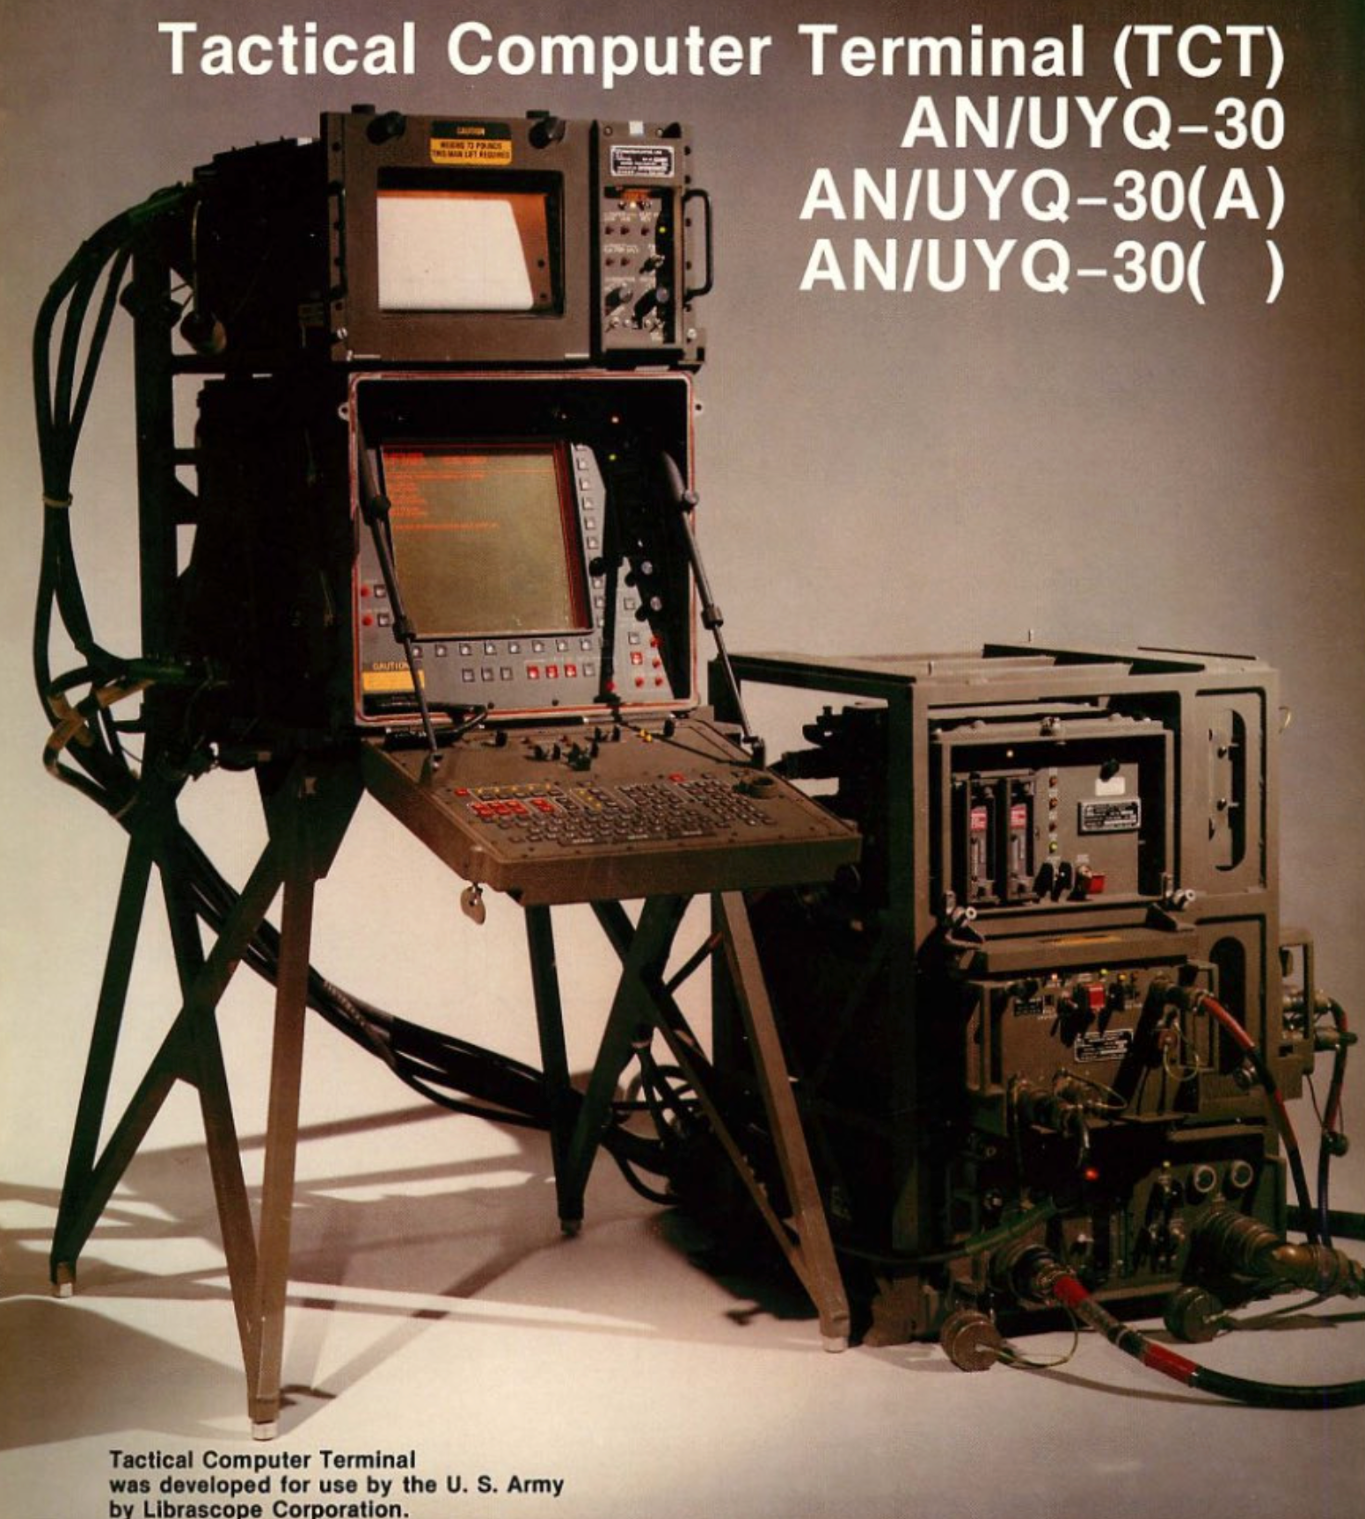
\includegraphics[width=2.75694in,height=3.08125in]{chapters/img/ch08/media/image1.png}Figure
1: Tactical Tech

Lorem ipsum dolor sit amet, consectetur adipiscing elit. Quisque nec
lobortis elit. Phasellus malesuada eleifend tempor. Maecenas
ullamcorper, metus efficitur commodo feugiat, diam libero rhoncus quam,
nec dapibus magna nunc id ligula. Aliquam eu libero facilisis, vulputate
augue quis, pretium nibh. Nullam eget eros at lorem bibendum tincidunt.
Morbi gravida finibus tellus, non posuere arcu fermentum id. Duis
iaculis accumsan est ac consectetur.

Maecenas hendrerit dui a varius pretium. Donec in purus eget ante
placerat suscipit. Aliquam pulvinar, turpis non egestas semper, lacus
nisi aliquam mauris, quis auctor metus ligula et sem. Ut a consequat
lacus, ac bibendum ligula. Pellentesque non imperdiet sem, et eleifend
nisi. Sed eu massa condimentum, fermentum arcu ac, viverra neque. In
imperdiet mi lectus, non mollis mi tincidunt a.

Vivamus mollis, tortor quis eleifend viverra, eros lorem pellentesque
justo, ut ornare diam magna id erat. Praesent commodo mi hendrerit elit
tincidunt malesuada. Integer tortor nisl, consequat et elit imperdiet,
sagittis porta tortor. Curabitur quam sem, ultrices id mauris et,
facilisis lacinia ex. Nunc tincidunt dictum orci, non sodales mi
facilisis sodales. Sed dictum felis dolor, at maximus sem volutpat
sagittis. Sed convallis eu mi id fringilla. Nullam sed lacinia diam.

Ut accumsan eget orci at ullamcorper. Morbi malesuada, lorem eu
facilisis gravida, sapien sem semper erat, ac mollis mauris nisl vel
est. Suspendisse lobortis turpis in enim interdum volutpat. Praesent
tempor tempor justo et vestibulum. Praesent ultrices mi sollicitudin,
blandit magna et, tristique erat. Nullam rutrum mi vehicula ullamcorper
suscipit. Sed feugiat, massa sit amet ultricies eleifend, nibh lectus
auctor augue, at consectetur nibh ligula ac purus. Nulla tristique,
mauris at vestibulum sollicitudin, diam sapien auctor est, non tempor
metus tortor ac risus. Interdum et malesuada fames ac ante ipsum primis
in faucibus. Donec id nisi nunc. In a interdum augue, quis lacinia urna.
Cras viverra neque vel vulputate aliquam. Sed mollis nisl quis dui
accumsan, non iaculis nunc luctus.

Vestibulum consectetur, mi et ultricies tincidunt, orci diam porta ex,
ut vestibulum magna dolor a dolor. Duis et velit erat. Integer maximus
erat ut sem porttitor, eu elementum ante congue. Cras id enim id orci
vehicula commodo vel sed mauris. Duis tellus dui, tempus fermentum leo
et, viverra suscipit felis. Mauris consequat sem commodo nisl sagittis,
euismod iaculis sapien molestie. Morbi lectus magna, ullamcorper sed
mauris eu, consequat interdum ipsum.

\bookmarksetup{startatroot}

\chapter*{Headers}\label{headers}
\addcontentsline{toc}{chapter}{Headers}

\markboth{Headers}{Headers}

\bookmarksetup{startatroot}

\chapter*{Header 1}\label{header-1}
\addcontentsline{toc}{chapter}{Header 1}

\markboth{Header 1}{Header 1}

\section*{Header 2}\label{header-2}
\addcontentsline{toc}{section}{Header 2}

\markright{Header 2}

\subsection*{Header 3}\label{header-3}
\addcontentsline{toc}{subsection}{Header 3}

\subsubsection*{Header 4}\label{header-4}
\addcontentsline{toc}{subsubsection}{Header 4}

\paragraph*{Header 5}\label{header-5}
\addcontentsline{toc}{paragraph}{Header 5}




\end{document}
